% !TEX program = xelatex
% =============================================================================
%  Andrew A. Port
%  An Introduction to Homological Mirror Symmetry and the Case of Elliptic Curves
%  arXiv:1501.00730v1 [math.SG]  (September 16, 2012)
%
%  中文译注版（结构化 LaTeX 源码）
%  编译：xelatex main.tex ，连续两遍
%  目录结构：
%      main.tex                 主文件（本文件）
%      preamble.tex             导言区：宏包、定理环境、keytakeaways、常用宏
%      sections/sec0.tex        引言
%      sections/sec1-2.tex      第 1–2 节
%      sections/sec3-5.tex      第 3–5 节
%      sections/sec6-7.tex      第 6–7 节（含图 6.1、6.2）
%      sections/sec8.tex        第 8 节
%      sections/appA-B.tex      附录 A、B 与参考文献
%      figures/fig6-1.png       原文 Figure 6.1（第 24 页）裁切图
%      figures/fig6-2.png       原文 Figure 6.2（第 26 页）裁切图
% =============================================================================
% =============================================================================
%  An Introduction to Homological Mirror Symmetry and the Case of Elliptic Curves
%  Andrew A. Port,  arXiv:1501.00730v1 [math.SG]  (UC Davis, September 16, 2012)
%
%  中文译注版 —— 导言区（preamble）
%  编译：xelatex main.tex  （连续编译两遍，以生成目录与页码）
%  依赖：TeX Live 2018+ / MiKTeX（ctex, amsmath, amssymb, amsthm, mathtools,
%        bm, amscd, tikz-cd, graphicx, caption, enumitem, xcolor, hyperref）
%  说明：ctex 会自动选择平台中文字体（Windows 下为宋体/黑体，Linux 下为 Fandol）。
%        如需强制指定，可用：
%        \usepackage[UTF8,fontset=windows,scheme=chinese]{ctex}
%        其他可选 fontset：mac, fandol, ubuntu, adobe。
% =============================================================================
\documentclass[11pt,a4paper]{article}

% ---------- 中文支持（XeLaTeX）----------------
\usepackage[UTF8,scheme=chinese]{ctex}

% ---------- 页面与版式 ------------------------
\usepackage[a4paper,top=2.6cm,bottom=2.6cm,left=2.7cm,right=2.7cm]{geometry}
\linespread{1.12}
\setlength{\parskip}{2pt plus 1pt}
\setlength{\emergencystretch}{2.5em}   % 避免中文长句与长公式造成的溢出

% ---------- 数学 ------------------------------
\usepackage{amsmath,amssymb,amsthm,mathtools,bm}
\usepackage{amscd}          % 简单交换图
\usepackage{tikz-cd}        % 复杂交换图（若本机无此宏包，可改用 amscd 并注释掉本行）
\allowdisplaybreaks[2]

% ---------- 图形与表格 ------------------------
\usepackage{graphicx}
\graphicspath{{figures/}{../figures/}}
\usepackage{caption}
\captionsetup{font=small,labelfont=bf,labelsep=quad,justification=centering}

% ---------- 列表 ------------------------------
\usepackage{enumitem}
\setlist[itemize]{leftmargin=1.6em,itemsep=1pt,topsep=2pt}
\setlist[enumerate]{leftmargin=1.8em,itemsep=1pt,topsep=2pt}

% ---------- 颜色与超链接 ----------------------
\usepackage{xcolor}
\usepackage[unicode=true,colorlinks=true,
            linkcolor=blue!45!black,citecolor=blue!45!black,urlcolor=blue!45!black,
            bookmarksnumbered=true,bookmarksopen=true]{hyperref}

% ---------- 中文名称（ctex 一般已自动设置，此处显式确保一致）----------
\renewcommand{\contentsname}{目录}
\renewcommand{\refname}{参考文献}
\renewcommand{\figurename}{图}
\renewcommand{\tablename}{表}
\renewcommand{\proofname}{证明}
\renewcommand{\abstractname}{摘要}

% 图号沿用原文的 “节号.序号” 形式（原文 Figure 6.1、6.2 → 图 6.1、6.2）
\renewcommand{\thefigure}{\thesection.\arabic{figure}}
% 第 8.5 节过宽的交换图：先存入盒子再等比缩放到版心宽度
\newsavebox{\widefigbox}

% ---------- 定理类环境 ------------------------
% 说明：原文各类环境共用一个“节内”编号（1.1, 1.2, ...），故下方让
%       theorem / lemma / proposition / corollary / definition / remark
%       共享同一计数器，并按原文出现顺序自动复现原编号。
\theoremstyle{plain}
\newtheorem{theorem}{定理}[section]
\newtheorem{lemma}[theorem]{引理}
\newtheorem{proposition}[theorem]{命题}
\newtheorem{corollary}[theorem]{推论}
\theoremstyle{definition}
\newtheorem{definition}[theorem]{定义}
\newtheorem{remark}[theorem]{注}
% 不编号环境
\newtheorem*{example}{例}
\newtheorem*{propositionstar}{命题}

% ---------- 每节“本节重点”盒子 -----------------
% 用法：\begin{keytakeaways} ... \end{keytakeaways}
%       （每节必写；内容为 3–5 条 itemize）
\newenvironment{keytakeaways}[1][本节重点]{%
  \par\addvspace{9pt}%
  \noindent\rule{\linewidth}{0.7pt}\par\nobreak
  \begin{quote}\noindent\textbf{#1}\par\small
}{%
  \end{quote}%
  \noindent\rule{\linewidth}{0.7pt}\par\addvspace{7pt}%
}

% ---------- 常用记号（可选，统一风格用）--------
\newcommand{\CC}{\mathbb{C}}
\newcommand{\RR}{\mathbb{R}}
\newcommand{\ZZ}{\mathbb{Z}}
\newcommand{\QQ}{\mathbb{Q}}
\newcommand{\OO}{\mathcal{O}}
\newcommand{\LL}{\mathcal{L}}
\newcommand{\FF}{\mathcal{F}}
\newcommand{\dd}{\mathrm{d}}
\newcommand{\Hom}{\operatorname{Hom}}
\newcommand{\Ext}{\operatorname{Ext}}
\newcommand{\End}{\operatorname{End}}
\newcommand{\GL}{\operatorname{GL}}
\newcommand{\Pic}{\operatorname{Pic}}
\newcommand{\Coh}{\mathrm{Coh}}
\newcommand{\vol}{\operatorname{vol}}
\newcommand{\tr}{\operatorname{tr}}
\newcommand{\id}{\operatorname{id}}

% ---------- 图表标题中的原文出处标记 -----------
% 用法：\caption{……。\origloc{原文 Figure 6.1，第 24 页}}
\newcommand{\origloc}[1]{\textnormal{（#1）}}


\begin{document}

% ---------------------------------------------------------------------------
%  标题页
% ---------------------------------------------------------------------------
\title{\bfseries 同调镜像对称导论\\[4pt] 与椭圆曲线情形}
\author{Andrew A. Port\\[2pt]
        \small Department of Mathematics, University of California, Davis\\[6pt]
        \small 中文译注与校订本}
\date{2012 年 9 月 16 日（原文）\\[2pt] 中译注版：2026 年}
\maketitle

\begin{abstract}
本文细致地构造了椭圆曲线上凝聚层的导出范畴与其镜像上某一版本深谷范畴之间的一个等价。这是同调镜像对称中最易理解的情形。我们同时为同调镜像对称猜想的一般卡拉比–丘情形提供入门性的背景。
\end{abstract}

\noindent\textbf{关键词：}镜像对称；同调镜像对称；深谷范畴；椭圆曲线；辛 $2$-环面

\vspace{1.2em}
\noindent\rule{\linewidth}{0.4pt}
{\small
\noindent\textbf{Original abstract.} Here we carefully construct an equivalence between the derived
category of coherent sheaves on an elliptic curve and a version of the Fukaya category on its
mirror. This is the most accessible case of homological mirror symmetry. We also provide introductory
background on the general Calabi--Yau case of The Homological Mirror Symmetry Conjecture.\par}
\noindent\rule{\linewidth}{0.4pt}

\vspace{0.6em}
\section*{译校说明}
\addcontentsline{toc}{section}{译校说明}

\begin{enumerate}
  \item 原文为 Andrew A. Port 在加州大学戴维斯分校的学位论文，arXiv:1501.00730v1 [math.SG]（2012 年 9 月 16 日），全文 43 页。译文保留原文章节、公式、定理与文献编号；定理类环境与公式编号已按原文顺序复现，便于与原文逐条对读。
  \item 术语依数学界通行译法统一（如 gauge theory 规范场论、holonomy 和乐、anomaly 反常、coherent sheaf 凝聚层、Fukaya category 深谷范畴）；人名首次出现时附原文拼写。原文中的引用编号（如 [37]）原样保留，参考文献条目保留英文原文。
  \item 源码中以 \texttt{\% [Tutor Note: ...]} 形式嵌入了学术性审校批注（易错符号约定、被省略证明的出处、原文笔误等）。这些批注是 LaTeX 注释，\emph{不参与排版}，可直接在源码中检索、增删。文末另附“译校札记与勘误表”集中列出所发现的原文问题。
  \item 原文 Figure 6.1（第 24 页）与 Figure 6.2（第 26 页）已从原 PDF 中裁切为 \texttt{figures/fig6-1.png}、\texttt{figures/fig6-2.png}，并以 \texttt{figure} 环境插入对应段落；图题已译为中文，并标注原文位置。
  \item 原文中个别公式在 PDF 文本层存在字形丢失（如 $\mathbb{C}$、$\mathcal{O}$、$\mathcal{L}$ 被压平为 \texttt{C}、\texttt{O}、\texttt{L}），译文均以原页面图像为准重新排印。
  \item 编译方式：XeLaTeX（\texttt{xelatex main.tex}，连续两遍）。若本机中文字体配置特殊，可在 \texttt{preamble.tex} 中改用
        \texttt{\textbackslash usepackage[UTF8,fontset=windows,scheme=chinese]\{ctex\}} 或 \texttt{fontset=fandol}。
  \item \textbf{记号提醒：}原文以 $E_\tau=\mathbb{C}/\Lambda$（下标）记 B 侧复环面，以 $E^{\rho}$、$E^{\tau}$、$E^{r\tau}$（上标）记 A 侧实环面，二者字形不同；PDF 文本层把上下标压平后无法区分。译文均按原页面图像还原为上标/下标。凡正文中 $E_\tau$ 与 $E^\tau$ 并存处，请按“下标 = B 侧复环面、上标 = A 侧辛环面”理解；原文亦有个别处误用上标记 B 侧（如第 26 页），已在对应批注中标明。
\end{enumerate}

\tableofcontents
\newpage

% ---------------------------------------------------------------------------
%  正文
% ---------------------------------------------------------------------------
% ===== 以下内容来自 sections/sec0.tex =====
% =============================================================================
%  §0  引言（Introduction）
%  对应原文：第 2–4 页
%  译者：Lead（含前置说明与全书统稿）
% =============================================================================
\setcounter{section}{-1}
\section{引言}

\begin{keytakeaways}
\begin{itemize}
  \item \textbf{物理图像：}镜像对称源于弦论——两个拓扑上不同的卡拉比–丘流形可以给出同一个量子场论、从而给出同一套物理。同调镜像对称（HMS）把这一“物理等价”提升为两个范畴之间的等价：A 侧（辛几何／深谷范畴）与 B 侧（复代数几何／凝聚层导出范畴）。
  \item \textbf{数学工具：}有界导出范畴、深谷范畴与 $A_\infty$-范畴、B-场与复化凯勒形式、以 $\theta$ 函数为基的态射集。
  \item \textbf{关键结论：}椭圆曲线情形（Polishchuk--Zaslow）是 HMS 目前最易理解且已获完整证明的案例；本文将显式构造 $D^b\mathrm{Coh}(E_\tau)$ 与 $H^0(\mathrm{Fuk}(E_\tau))$（形式上添加双积后）之间的等价函子，其核心是把伪全纯圆盘的计数翻译为 $\theta$ 函数的加法公式。
\end{itemize}
\end{keytakeaways}

镜像对称\footnote{“镜像对称”一词当然远更早便被用于描述数学中其他概念。本论文所研究的镜像对称概念，得名于在某些流形对的霍奇菱形（Hodge diamond）中观察到的一种对称性。自命名以来，该领域已发生相当剧烈的演变，但名称保留至今。}这一概念，就其最早形态而言，是 20 世纪 80 年代末由物理学家提出的。他们注意到，拓扑上不同的流形可以给出等价的量子场论，从而给出等价的物理。

1994 年，即这些最初观察之后约十五年\footnote{关于这十五年间该领域演变的史料性叙述很多（例如 [47] 第 7 章）。}，孔采维奇（Kontsevich）提出了该对称性的一个数学严格框架，其基础就是如今所称的\emph{同调镜像对称猜想}（The Homological Mirror Symmetry Conjecture）[29]。[29] 中提出的主要猜想，可以看作是对“卡拉比–丘流形的镜像对偶”这一说法给出定义。该定义（较其原始形式略有减弱）可表述如下。

设 $X$ 为卡拉比–丘流形。称复代数流形 $\tilde X$ 与 $X$ \emph{镜像对偶}，若 $\tilde X$ 上凝聚层的有界\footnote{如镜像对称语境中常见的那样，我们一般会省略“有界”一词，简称“导出范畴”。}导出范畴，等价于由 $X$ 的深谷范畴“（或它的某个适当扩大）”构造的有界导出范畴。

$X$ 的（导出）深谷范畴只由 $X$ 的凯勒结构（与一个 B-场耦合）构造，而 $\tilde X$ 上凝聚层的（导出）范畴只依赖于 $\tilde X$ 的复结构。特别地，同调镜像对称（HMS）是辛几何与代数几何之间的一种关系。\footnote{本论文通篇常把这两侧（辛侧与代数几何侧）分别称为 A 侧与 B 侧。这一术语来自把镜像对称解释为 IIA 型与 IIB 型弦论之间对偶的弦论图像。}

目前人们“普遍相信”（[15] 第 1.4 节），每个卡拉比–丘流形都存在这样的镜像对偶，且该对偶也是卡拉比–丘流形。

就卡拉比–丘流形而言，如上述表述，这一等价（或其近似版本）已在椭圆曲线 [37] 与（$X$ 为）四次曲面 [38] 的情形得到完整证明。该猜想的若干方面已在其他情形得到证明，特别是阿贝尔簇与拉格朗日环面纤维化的情形 [14, 30]。此外还有把 HMS 推广到非卡拉比–丘流形的种种猜测（例如 [2, 26]）：其中辛流形的镜像对偶被取为由复簇 $\tilde X$ 与全纯函数 $W$ 组成的对\footnote{对 $(\tilde X,W)$ 称为朗道–金兹堡模型（Landau--Ginzburg model），函数 $W$ 称为朗道–金兹堡超势。} $(\tilde X,W)$。对于亏格 $g\ge 2$ 的所有曲面，这一更一般的 HMS 已有完整证明 [39, 10]）\footnote{亏格零情形的完整证明也可能已经存在，或隐含在相关工作之中（该情形的综述见 [3]）。}\footnote{作者为任何他未能知晓的完整证明致歉，也为上述文献未收录的、卡拉比–丘与非卡拉比–丘两类情形中的许多部分结果致歉。}
% [Tutor Note: 含糊点 —— 原文称“所有亏格 g≥2 的曲面”都已完整证明，但所引文献 [39]（Seidel, 亏格 2）与 [10]（Efimov, 高亏格）实际覆盖的情形并不等同于“所有 g≥2”这一断言；这是作者的综述性表述，译文按原文译出，读者引用时宜回到 [39, 10] 核对。]
% [Tutor Note: 易错点 —— 这里“有界导出范畴”与“由深谷范畴构造的导出范畴”是两类不同对象：后者须取深谷 A∞-范畴的（有界）导出范畴或适当的扩大（enlargement），Kontsevich 原文对此有明确限定。原文用引号标出 “or a suitable enlargement of it”，译文保留引号，请勿将其误解为普通的有界导出范畴。]

本论文将集中于 HMS 的卡拉比–丘情形。我们将以 $X$ 为椭圆曲线\footnote{椭圆曲线（即一维复环面）是唯一的一维卡拉比–丘流形。}的例子来介绍这一主题。这一情形之所以特别容易掌握，是因为椭圆曲线是理解得特别透彻的几何对象；本文的目的在于提供足够详细（并以足够入门的层次呈现）的说明，使一位几何取向的数学家能够较好地理解这一情形及其背后更一般的猜想（而不必先具备通常与 HMS 相伴的那些庞杂而多样的预备知识）。我们将特别注意给出与 [37, 31] 中已有论述互补的解释，并且只要不偏离理解椭圆曲线情形这一目标太远，就尽力以一般卡拉比–丘情形来表述我们的解释。

在孔采维奇提出其原始 HMS 猜想的 ICM 报告 [29] 中，他还就椭圆曲线情形下这一范畴等价的两侧给出了粗略比较。约五年后，波利舒克（Polishchuk）与扎斯洛夫（Zaslow）在一种减弱的情形下给出了该情形的证明，本文将对之加以描述。

简述如下：设 $\tau=b+iA\in\mathbb{R}\oplus i\mathbb{R}_{>0}$，以 $E_\tau$ 记光滑 2-环面配上辛形式 $A\,\mathrm{d}x\wedge\mathrm{d}y$ 以及另一个 2-形式 $b\,\mathrm{d}x\wedge\mathrm{d}y$，后者称为“B-场”。$E_\tau$ 的镜像对偶是由格 $\Lambda=\langle 1,\tau\rangle$ 的自然作用给出的复 1-环面 $E_\tau:=\mathbb{C}/\Lambda$。
% [Tutor Note: 易错点 —— 原文在此处对 A 侧（带辛形式与 B-场的实 2-环面）与 B 侧（复环面 $\mathbb{C}/\Lambda$）使用了同一个记号 $E_\tau$，这是原文的记号混用；自第 5.1 节起作者将 A 侧改记为 $E^\rho$（上标，$\rho=B+iA$），B 侧仍记 $E_\tau$。阅读时务必按上下文（辛侧/复侧）区分，切勿把两侧的 $E_\tau$ 当作同一对象。]

上面提到的“减弱情形”，是指深谷范畴的零次上同调 $H^0(\mathrm{Fuk}(E_\tau))$（形式上添加双积）与凝聚层导出范畴 $D^b\mathrm{Coh}(E_\tau)$ 之间的等价。\footnote{确切地说，这将是一个加性范畴之间的等价。一般而言，深谷范畴并非真正的范畴，而是仅在（上）同调层面结合的 $A_\infty$-范畴（更糟时是弯曲 $A_\infty$-范畴）。然而在这一维情形，其结合性的障碍消失；并且在形式上添加双积之后，我们可以构造与凝聚层导出范畴的等价，而无需考虑扩大为由深谷范畴构造的导出范畴。}这两个范畴之间的函子，将由一个出奇地奇特的关系构造出来：它把 $E_\tau$ 上配以平坦复向量丛（以及某些附加结构）的闭测地线，送到全纯向量丛与挠层。

事实上，不可分解的挠层将是竖直测地线（即 $\mathbb{R}^2/\mathbb{Z}^2$ 商映射下竖直直线的投影）的像。态射的像则由一个把（测地线的）交点送到 $\theta$ 函数的关系来描述！也许最重要的是：由于深谷范畴中态射的复合由交点的形式和给出，其系数来自对（以交点为标记点的）伪全纯圆盘的计数，该函子把这一计数信息编码进（某些凝聚层的态射复合，而这些复合可用）$\theta$ 函数的线性组合（系数为常矩阵）之中。

本论文组织如下。第 1 节简要回顾辛几何与复几何中必要的背景与定义；第 2 节继续简要讨论复向量丛与全纯向量丛理论中必要的背景。第 3、4 节给出所有必要几何结构的详细构造，以及椭圆曲线上所有全纯线丛。第 5、6 节讨论深谷范畴，并共同给出对 [37] 中“最简单的例子”——即 HMS 最简例子——的详细阐述。第 7、8 节讨论椭圆曲线上凝聚层的导出范畴，并构造上述该范畴与 $H^0(\mathrm{Fuk}(E_\tau))$ 的某个扩大之间的函子。我们还包含两个附录：第一个是对一般导出范畴的极简回顾，第二个是对特殊拉格朗日子流形及相关几何的入门介绍。

\subsection*{致谢}

作者感谢学位论文委员会的成员 Jerry Kaminker、Motohico Mulase 与 Andrew Waldron；也感谢许多曾花时间教作者数学的教授与研究生，尤其是 Andrew Waldron 与 David Cherney——他们花了无数小时试图教会作者量子场论；以及 Michael Penkava——他把作者首次引向镜像对称的同调观点。最后，作者再次感谢导师 Motohico Mulase，他为培养作者成为一名数学家付出了大量心血。
% --- 译者交付说明：§0 覆盖原文第 2–4 页；脚注 9 条（原编号 1–9 全部译出）；批注 3 条；原文中 “thesis” 一词按硕士论文译作“本论文”。原文将 [28] 之后的引用写为普通方括号，译文保留。---

% ===== 以下内容来自 sections/sec1-2.tex =====
\section{复流形、辛流形与凯勒流形}
% 本片段：§1（复流形、辛流形与凯勒流形）与 §2（复向量丛与全纯向量丛），
% 对应原文第 4–13 页；原文第 14 页页首已是 §3，不在本片段内。

\begin{keytakeaways}
\begin{itemize}[leftmargin=1.6em,itemsep=1pt,topsep=2pt]
  \item \textbf{几何图像：}本节搭起全篇的三层几何舞台——复流形（全纯图册、殆复结构及其可积性）、辛流形（闭而非退化的 2-形式）与凯勒流形（二者相容）；卡拉比–丘流形进一步要求存在处处非零的全纯 $n$-形式，这正是超弦理论中额外六维紧化空间的几何要求。
  \item \textbf{数学工具：}奈恩黑斯张量判定殆复结构的可积性（定理 1.1）；达布定理给出辛结构的局部标准形（定理 1.6）；李导数的嘉当公式把辛向量场与闭 1-形式联系起来；哈密顿流用来定义拉格朗日子流形的哈密顿等价（定义 1.9）。
  \item \textbf{关键结论：}所有辛流形局部全同（达布）；凯勒条件有“$\omega$ 闭且 $J$ 可积”“$\nabla J=0$”“$\nabla\omega=0$”三种等价表述（定义 1.10）；第一陈类为零的紧凯勒流形上存在唯一的上同调等价的 Ricci 平坦凯勒结构（定理 1.11，即丘成桐证明的卡拉比猜想）。
\end{itemize}
\end{keytakeaways}

本节将对复流形、辛流形与凯勒流形作一些非常基本的回顾。

\subsection{复流形}

复流形是一个光滑的 $2n$ 维流形 $M$，带有一个把 $M$ 映入 $\mathbb{C}^n$ 的图册，使得其转移函数全纯。等价地，$M$ 是一个容许复结构（定义见下）的光滑流形。

\begin{example}
$\mathbb{C}^n$ 是复流形，其单图图册由恒等映射给出。
\end{example}

\begin{example}
$\mathbb{CP}^n$ 是复流形，其图册由映射
\[
\phi_i\colon [t_0,\ldots,t_{i-1},1,t_{i+1},\ldots,t_n]\to (t_1,\ldots,t_{i-1},t_{i+1},\ldots t_n)
\]
给出。
\end{example}

% [Tutor Note: 原文勘误 —— 原印 $\phi_i$ 的像点坐标为 $(t_1,\ldots,t_{i-1},t_{i+1},\ldots t_n)$，按 $\mathbb{CP}^n$ 齐次坐标的标准约定（令第 $i$ 个坐标等于 $1$ 后删去它）应为 $(t_0,\ldots,\widehat{t_i},\ldots,t_n)$，且末尾缺一个逗号；译文按原文排印。另，“紧连通子流形必为点”一句省略了论证：$\mathbb{C}^m$ 的坐标函数限制在紧子流形上全纯且有界，由刘维尔定理为常数，故子流形只能是单点。]

复流形与光滑流形之间的一个重要区别在于：并非所有复流形都是 $\mathbb{C}^m$ 的子流形。事实上，由刘维尔定理，$\mathbb{C}^m$ 的任何紧连通子流形都是一个点。

\subsection{殆复结构}

我们可以通过选取满足 $J^2=-1$ 的线性映射 $J\colon V\to V$，把任何偶数维向量空间 $V$ “复化”。这赋予 $V$ 一个复向量空间结构，其乘法由 $(a+ib)\cdot v=(a+Jb)v$ 定义。

一个光滑流形 $M$ 若容许一个平方为负恒等映射的光滑切丛同构 $J\colon TM\to TM$（称为殆复结构），则称 $M$ 为殆复的。所有复（以及辛）流形都容许殆复结构，但反之不成立（无论对复流形还是对辛流形而言）。

更具体地说，在殆复流形 $(M,J)$ 上，我们总能找到复坐标 $z^\mu=x^\mu+iy^\mu\colon M\to\mathbb{C}$，使得在给定点 $p\in M$ 处有
\[
J\frac{\partial}{\partial x^\mu}=i\frac{\partial}{\partial y^\mu}
\qquad\text{以及}\qquad
J\frac{\partial}{\partial y^\mu}=-\frac{\partial}{\partial x^\mu}.
\]
然而，一般来说不可能找到使上式在 $p$ 的整个邻域内都成立的坐标。如果围绕每一点 $p$ 都能在其邻域内找到这样的坐标，那么这些坐标会黏合起来构成 $M$ 的全纯图册，此时 $J$ 称为一个复结构。

\begin{theorem}[纽兰德–尼伦伯格定理 {[35]}]
殆复流形 $(M,J)$ 是复结构为 $J$ 的复流形，当且仅当奈恩黑斯张量消失，即
\[
N_J(v,w):=[v,w]+J[v,Jw]+J[Jv,w]-[Jv,Jw]\equiv 0
\]
对所有 $v,w\in\Gamma(TM)$ 成立，其中 $[\cdot,\cdot]$ 是 $M$ 上向量场的李括号。
\end{theorem}

% [Tutor Note: 省略证明 —— 定理 1.1 未给证明，其核心是把 $J$ 的可积性化归为一阶偏微分方程组（$\bar\partial$-方程）的局部可解性，标准处理见 [35] 原文或 Kobayashi–Nomizu《Foundations of Differential Geometry》Vol. II 的复流形一章。原文勘误 —— 定理标题印作 “Newlander-Niremberger”，应为 “Newlander–Nirenberg”（参考文献 [35] 的拼写即为 Newlander–Nirenberg）。]

\begin{example}
曲面上的所有殆复结构都是可积的。
\end{example}

\begin{remark}
所有辛流形都容许殆复结构。事实上，给定辛流形 $(M,\omega)$，无论选取殆复结构 $J$ 还是黎曼度量 $g$，都定义了一个“相容三元组”$(\omega,J,g)$，使得 $g(u,v)=\omega(u,Jv)$。
\end{remark}

% [Tutor Note: 易错符号约定 —— 本文全篇采用 $g(u,v)=\omega(u,Jv)$；若改用 $g(u,v)=\omega(Ju,v)$ 或 $\omega(u,v)=g(Ju,v)$，则相容三元组中 $J$ 的旋转方向与辛形式的整体符号相反，后文哈密顿向量场的符号也会随之改变。原文勘误 —— 上文“复化”的乘法公式印作 $(a+ib)\cdot v=(a+Jb)v$，按含义应为 $(a+ib)\cdot v=av+bJv$。]

\begin{definition}
设 $f\colon M\to M'$ 是殆复流形 $(M,J)$ 与 $(M',J')$ 之间的映射。若 $df\circ J=J'\circ df$，则称 $f$ 是 $(J,J')$-全纯的（原文如此，原印作 “$df\,J=J'f$”）。
\end{definition}

\subsection{辛几何}

辛几何的研究最初由哈密顿力学领域所推动：该领域试图用辛流形上的“守恒量”（见 §1.4）来描述经典力学的规律，而该辛流形代表某个系统所有可能的位置与动量取值构成的空间。“symplectic”一词由外尔（Weyl）于 1939 年引入（见 [43] 第 165 页的脚注），作为“complex”的拉丁词根（意为“编织在一起的”，braided）的希腊语对应词。尽管渊源如此之早，直到 1985 年格罗莫夫（Gromov）引入伪全纯曲线的思想之前，人们对辛几何所知甚少。此后，格罗莫夫–威滕不变量与弗洛尔同调大大拓展了我们理解这些几何的数学结构的能力。

\begin{definition}
辛流形是一对 $(M,\omega)$，其中 $M$ 是光滑流形，$\omega$ 是 $M$ 上的闭、非退化 2-形式。我们把这样的 $\omega$ 称为一个辛形式。
\end{definition}

\begin{remark}
这个反对称形式的非退化性要求所有辛流形都是偶数维的，并且对每个 $p\in M$，$T_pM$ 都存在基 $e_1,\ldots,e_n,f_1,\ldots,f_n$，使得 $\omega(e_i,f_j)=\delta_{ij}$，且 $\omega(e_i,e_j)=\omega(f_i,f_j)=0$ 对所有 $i,j$ 成立。
\end{remark}

例子：
\begin{itemize}
  \item $2n$ 维欧氏空间：$\mathbb{R}^{2n}$ 带其标准坐标与 $\omega=\sum_{i=1}^n\mathrm{d}x_i\wedge\mathrm{d}x_{i+n}$。
  \item 任何带任何非零 2-形式的 2 维曲面。
  \item $2n$-环面\footnote{在给它赋予复结构之后，我们将把这个流形称为复 $n$-环面；当 $n=1$ 时，称为椭圆曲线。}：$\mathbb{C}^n/\underbrace{\mathbb{Z}^{2n}}_{2n\text{ 次}}\cong S^1\times\cdots\times S^1$ 带其标准角坐标与 $\omega=\sum_{i=1}^n\mathrm{d}\theta_i\wedge\mathrm{d}\theta_{i+n}$（原文如此，原印作 “$\sum_{i=1}^n\omega=\mathrm{d}\theta_i\wedge\mathrm{d}\theta_{i+n}$”）。
  \item 任何光滑 $n$ 维流形 $M$ 的余切丛 $T^*M$ 都可赋予辛结构。用 $(x_1,\ldots,x_n)$ 表示 $M$ 上的局部坐标，我们可以通过映射
\[
(x,\xi)\mapsto (x_1,\ldots,x_n,\xi_1,\ldots,\xi_n)
\]
在 $T^*M$ 上定义局部坐标，其中 $\xi_i$ 是 $\xi$ 关于局部坐标基形式的分量，即 $\xi=\sum\xi_i\,\mathrm{d}x_i$。于是 $\omega=\sum\mathrm{d}x_i\wedge\mathrm{d}\xi_i$ 定义了 $T^*M$ 上的一个辛形式。
\end{itemize}

非例：
\begin{itemize}
  \item 任何奇数维流形或不可定向流形。
  \item 由斯托克斯定理：任何第二上同调为零的紧连通流形（例如 $n>2$ 时的 $S^n$）。此时辛形式必须是恰当的，于是令 $\eta$ 表示其原函数，就得到恰当的体积形式 $\omega^n=\mathrm{d}(\eta\wedge\omega^{n-1})$。
\end{itemize}

% [Tutor Note: 省略证明 —— 定理 1.6 只给出文献指引，标准证明用 Moser 同伦论证（取 $\omega_t=\omega+t(\omega_0-\omega)$，用闭形式的 Poincaré 引理逐点构造向量场并积分），见 [9]。原文勘误 —— 上文 “braded together” 应为 “braided together”；“Stoke's theorem” 应为 “Stokes' theorem”。另，环面例子中原文把求和号写在 $\omega$ 的左侧（$\sum_{i=1}^n\omega=\mathrm{d}\theta_i\wedge\mathrm{d}\theta_{i+n}$），按上下文应为 $\omega=\sum_{i=1}^n\mathrm{d}\theta_i\wedge\mathrm{d}\theta_{i+n}$，译文已按更正后的写法排印并在正文括注原文。]

\begin{theorem}[达布定理]
\sloppy
设 $(M,\omega)$ 是 $2n$ 维辛流形，$p\in M$。则存在局部坐标卡 $(U,(x_1,\ldots,x_n,y_1,\ldots,y_n))$，使得 $p\in U$，且在 $U$ 上
\[
\omega=\sum_{i=1}^n\mathrm{d}x_i\wedge\mathrm{d}y_i .
\]
\end{theorem}
\begin{proof}
该定理的证明可在大多数辛几何入门教材中找到（例如 [9]）。
\end{proof}

\begin{remark}
这说明所有辛流形局部看起来都一样。作为对照，任何黎曼度量都可以（通过选取坐标）在单个点处看起来像欧氏度量，但未必在整个邻域内如此。如果围绕每一点都能找到这样的局部坐标片，那么按定义我们的流形是平坦的。
\end{remark}

\subsection{拉格朗日子流形与哈密顿流}

深谷范畴的对象是闭拉格朗日子流形（带有我们稍后将描述的一些附加结构）。这些子流形通常要么被要求是“特殊的”（按附录 B 中描述的意义），要么只在下面将要描述的“哈密顿等价”意义下被考虑。

\begin{definition}
设 $(M,\omega)$ 是辛流形。若 $\omega|_L\equiv 0$，则称子流形 $L\subset M$ 为拉格朗日子流形。
\end{definition}

设 $V$ 是光滑流形 $M$ 上的任意向量场。我们可以局部地（在时间上）解出点 $x\in M$ 沿 $V$ 方向的“流”（即解 $\dot\gamma(t)=V_{\gamma(t)}$，$\gamma(0)=x$）。容易证明，这给出了一族微分同胚 $\psi_t\colon M\to M$，称为 $V$ 的流。若 $V$ 的流对所有时间都存在，则称 $V$ 是完备的。辛流形 $(M,\omega)$ 上的向量场 $V$ 若其流保持 $\omega$（即 $\psi_t^*\omega=\omega$），则称为辛向量场。由李导数的嘉当公式，我们有
\[
\frac{\mathrm{d}}{\mathrm{d}t}\psi_t^*\omega=\operatorname{Lie}_V\omega=\mathrm{d}(V\lrcorner\,\omega)+V\lrcorner\,\mathrm{d}\omega=\mathrm{d}(V\lrcorner\,\omega),
\]
其中我们用 $\lrcorner$ 表示内积，即 $V\lrcorner\,\omega\colon W\mapsto\omega(V,W)$。

% [Tutor Note: 易错符号约定 —— 此处内积约定为 $V\lrcorner\,\omega\colon W\mapsto\omega(V,W)$（第一个变量缩并），于是哈密顿向量场由 $\mathrm{d}H=V\lrcorner\,\omega$ 定义，即 $\omega(V,\cdot)=\mathrm{d}H$；若改用 $\omega(\cdot,V)=\mathrm{d}H$ 的约定，则所有哈密顿向量场整体差一个符号，哈密顿等价的定义与后文辛同调中的定向约定都须相应调整。]

这告诉我们：$V$ 是辛向量场当且仅当 $V\lrcorner\,\omega$ 是闭的。若 $V\lrcorner\,\omega$ 恰当，则存在函数 $H\colon M\to\mathbb{R}$ 使得 $\mathrm{d}H=V\lrcorner\,\omega$。此外，这个函数 $H$ 被流保持，即 $\frac{\mathrm{d}}{\mathrm{d}t}\psi_t^*H=\mathrm{d}H(V)=0$。此时 $\psi_t$ 称为哈密顿流，$H$ 称为哈密顿函数，$V$ 称为哈密顿向量场。

注意 $\omega$ 在向量与余向量之间定义了一个完美配对。因此给定任意函数 $H$，我们都能找到向量场 $V$ 使得 $\mathrm{d}H=V\lrcorner\,\omega$。

\begin{definition}
两个拉格朗日子流形 $L$ 与 $L'$ 称为哈密顿等价的，若存在哈密顿流 $\psi\colon I\times M\to M$，使得对某个 $t\in I$ 有 $\psi_t(L)=L'$。
\end{definition}

\subsection{凯勒几何}

殆复流形切丛上光滑变化的、正定的埃尔米特内积称为埃尔米特度量。带有这种结构的（相应地，殆）复流形称为（殆）埃尔米特流形。

殆埃尔米特流形 $(M,J,h)$ 具有一个相伴的黎曼度量与非退化 2-形式，它们分别由 $h$ 的对称部分与反对称部分给出，即 $g=\frac{1}{2}(h+\bar h)$ 与 $\omega=\frac{i}{2}(h-\bar h)$。此外，由于任何光滑流形都容许黎曼度量 $g$，殆复结构 $J$ 的存在就给出非退化 2-形式 $\omega(X,Y)=g(JX,Y)$ 的存在，从而给出埃尔米特度量 $h=g-i\omega$。

\begin{definition}
凯勒流形是满足某一可积性条件的殆埃尔米特流形，该条件可以写成以下三种等价形式：
\begin{itemize}
  \item $\omega$ 是闭的且 $J$ 可积；
  \item $\nabla J=0$；
  \item $\nabla\omega=0$，
\end{itemize}
其中 $\nabla$ 是 $g$ 的列维-奇维塔联络。
\end{definition}

% [Tutor Note: 易错符号约定 —— 原文取 $g=\frac{1}{2}(h+\bar h)$、$\omega=\frac{i}{2}(h-\bar h)$，即 $h=g-i\omega$；不少教材把凯勒形式直接写成 $\omega=\frac{i}{2}\sum h_{\alpha\bar\beta}\,\mathrm{d}z^\alpha\wedge\mathrm{d}\bar z^\beta$，与本文 $h=g-i\omega$ 的约定对读时若不注意，会差一个因子 2（或整体符号）。另，三种等价表述之所以等价，前提是 $\omega(\cdot,\cdot)=g(J\cdot,\cdot)$ 且 $J$ 与 $g$ 相容（$g(JX,JY)=g(X,Y)$）——原文未说明这一前提。原文勘误 —— “Levi-Cevita” 应为 “Levi-Civita”。]

\begin{example}
所有黎曼曲面都是凯勒流形。
\end{example}

\subsection{卡拉比–丘流形}

卡拉比–丘流形至少自 1950 年代起就为数学家所研究 [5, 6]，而自 1980 年代起 [7]，它对研究超弦理论的物理学家尤为重要。超弦理论是一种统一理论，它试图通过把粒子建模为振动的弦来描述所有基本粒子与自然界的基本力。为使超弦模型成为自洽的物理理论（例如能预言无质量的光子），时空必须是十维的。实验观测使我们相信，我们的时空局部看起来像四维闵可夫斯基空间 $M^4$（即带伪黎曼度量 $\mathrm{d}\vec{x}^2-\mathrm{d}t^2$ 的 $\mathbb{R}^4$）。因此，若这额外六维确实存在，则人们预期时空局部看起来像乘积 $M^4\times X$，其中 $X$（不正式地说）是某个具有极小长度尺度（普朗克长度量级）的紧空间。$X$ 的不同选取（当然还有乘积结构的不同选取）导致不同的“有效”四维理论。[7] 中证明：在关于时空乘积结构的某些假设下，为使这一有效四维理论容许 $N=1$ 超对称（物理学家普遍希望具有的性质），$X$ 必须取为卡拉比–丘流形。

我们把 $n$ 维卡拉比–丘流形定义为容许处处非零的全纯 $n$-形式的紧 $n$ 维凯勒流形，并称该 $n$-形式为其卡拉比–丘形式。

卡拉比–丘的这一定义蕴含我们的凯勒结构具有消失的第一陈类，从而由“卡拉比猜想”可以看作 Ricci 平坦的；我们在此把该猜想作为已由丘成桐（Yau）[45, 46] 证明的定理陈述如下。

\begin{theorem}
设 $M$ 是容许凯勒形式 $\omega$ 的紧复流形，并设 $\rho'$ 是 $M$ 上某个实的、闭的 $(1,1)$-形式，使得 $[\rho']=2\pi c_1(M)$。则 $M$ 上存在唯一的凯勒形式 $\omega'$，使得 $[\omega]=[\omega']\in H^2(M,\mathbb{R})$，且 $\rho'$ 是 $\omega'$ 的 Ricci 形式。特别地，若第一陈类在 $M$ 上消失（相对于某个凯勒度量），则 $M$ 容许唯一的、上同调等价的 Ricci 平坦（即 $\rho=0$）凯勒结构。
\end{theorem}

% [Tutor Note: 省略证明 —— 定理 1.11 即卡拉比猜想（丘成桐定理），原文未给证明，核心是把 Ricci 形式的条件化为复 Monge–Ampère 方程 $\det(g_{i\bar j}+\partial_i\bar\partial_{\bar j}\varphi)=\det(g_{i\bar j})e^{f}$ 的 $C^\infty$ 可解性（先验估计 + 连续性方法），见 [45, 46] 或 [47] 第 6–7 章的通俗介绍。易错符号约定 —— 原文写 $[\rho']=2\pi c_1(M)$；Ricci 形式有 $\rho=-\mathrm{i}\partial\bar\partial\log\det(g)$ 与 $\rho=+\mathrm{i}\partial\bar\partial\log\det(g)$ 两种约定，相差整体符号，采用相反约定时定理中的 $2\pi c_1(M)$ 应换成 $-2\pi c_1(M)$，请核对所引文献的约定。]

\begin{example}
在一维情形，这推出我们的紧黎曼曲面是可平行化的。因此唯一的例子是亏格为一的曲面。
\end{example}

\section{复向量丛与全纯向量丛}

\begin{keytakeaways}
\begin{itemize}[leftmargin=1.6em,itemsep=1pt,topsep=2pt]
  \item \textbf{几何图像：}B 侧（复几何侧）所研究的层、线丛与全纯向量丛都建立在向量丛之上；而带平坦联络的向量丛（局部系统）是 A 侧拉格朗日对象上附加的“规范数据”，两侧的信息在此交汇，为同调镜像对称中“拉格朗日子流形配局部系统”的表述作准备。
  \item \textbf{数学工具：}用转移函数与拼接函数（clutching function）分类复向量丛（定理 2.3）；用单值表示与和乐群描述平坦联络（定理 2.7、推论 2.9）；线丛–除子对应（定理 2.13）；格罗滕迪克消没定理（定理 2.14）、黎曼–罗赫定理（定理 2.16）与塞尔对偶（定理 2.17）。
  \item \textbf{关键结论：}$S^k$ 上的复向量丛由 $\operatorname{GL}_k(\mathbb{C})$ 值映射的同伦类分类；$S^1$ 上秩 $k$ 平坦联络的规范等价类对应 $\operatorname{GL}_k(\mathbb{C})$ 的共轭类；亏格 $g$ 黎曼曲面上 $\operatorname{Pic}(C)\cong\mathbb{Z}\times J(C)$；在亏格一的紧黎曼曲面上 $\deg(\mathcal{V})=h^0(\mathcal{V})-h^1(\mathcal{V})=h^0(\mathcal{V})-h^0(\mathcal{V}^*)$（注 2.18）。
\end{itemize}
\end{keytakeaways}

研究同调镜像对称需要很好地理解复向量丛与全纯向量丛。我们在此对这些主题作一些简要回顾，只涉及与本论文相关的部分。

\subsection{复向量丛}

\begin{definition}
秩为 $k$ 的复向量丛是一个向量丛 $\mathbb{C}^k\to E\xrightarrow{\pi}M$，其转移函数是 $\mathbb{C}$-线性的。
\end{definition}

\begin{example}
平凡丛 $M\times\mathbb{C}^k\xrightarrow{\operatorname{proj}_1}M$ 是秩 $k$ 复向量丛。殆复流形的复化切丛也是复向量丛。这两个例子很少相同。事实上，复（一维）环面是唯一使二者相同的黎曼曲面（对 $k=1$）。
\end{example}

让我们分类 $k$-球面上的所有复向量丛。

\begin{lemma}
可缩底空间上的每个向量丛都是平凡的。
\end{lemma}
\begin{proof}
若不然，我们对向量丛的定义就没有意义了。
\end{proof}

\begin{theorem}
映射 $f\colon S^{k-1}\to\operatorname{GL}_k(\mathbb{C})$ 的同伦类，与 $S^k$ 上的复向量丛之间存在一一对应。
\end{theorem}
\begin{proof}
设 $E\to S^k$ 是任意秩 $n$ 复向量丛。由上述引理，$E$ 可被两个平凡化覆盖，$\psi_\pm\colon\pi^{-1}(D^k_\pm)\to D^k_\pm\times\mathbb{C}^n$，其中 $D_+\cap D_-\cong(-\epsilon,\epsilon)\times S^{k-1}$。于是这个两图图册的转移函数由同伦 $f_t\colon S^{k-1}\to\operatorname{GL}_k(\mathbb{C})$（$t\in(-\epsilon,\epsilon)$）给出。\footnote{当然，给定一组完整的转移函数，我们可以重构出它们所来自的丛。这个同伦 $f_t$ 有时称为拼接函数（clutching function）。}于是剩下的只需说明这个同伦类是良定义的，即若取任意两个图册，得到的同伦类相同。为此注意到，我们可以把 $\phi_\pm$ 收缩为单点上的常值映射。由于 $\operatorname{GL}_n(\mathbb{C})$ 是道路连通的，所有这些图册都同伦等价。\footnote{另一方面，$\operatorname{GL}_n(\mathbb{R})$ 不是只有一个而是有两个道路连通分支。不过我们同样可以分类 $k$-球面上所有可定向的实向量丛。}
\end{proof}

\begin{remark}
由此可知，圆周上所有复向量丛都是平凡的（从证明中也可看出，实丛结构有两种选择——柱面或莫比乌斯带）。上述技巧可用于任何能被两个可缩图覆盖的流形。例如，$\mathbb{C}^*$ 上的所有丛也是平凡的。事实上，我们可以把这一点推广（正如 [4] 最后所做的那样）到具有由 $r$ 个图组成的“良”覆盖的流形（即有限型流形），从而得到秩 $k$ 复向量丛与映射 $M\to\operatorname{Gr}_k(\mathbb{C}^n)$（对任意 $n\ge rk$）的同伦类之间的双射。事实上，我们可以用无穷格拉斯曼流形来分类任意流形上的复向量丛（见 [21]）。
\end{remark}

设 $E\to M$ 是 $n$ 维流形 $M$ 上实的秩 $k$ 向量丛。若 $k>n$，则 $E$ 存在处处非零的全局截面。类似地，若 $E$ 是复的且纤维为 $\mathbb{C}^k$，则当 $k>n/2$ 时存在全局截面。特别地，这告诉我们任何向量丛都形如 $E=E'\oplus I_{k-n}$，其中 $I$ 是平凡丛，$E'$ 是某个纤维为 $n$ 维的丛。

注意，取 $E$ 的任意截面，我们都可以用横截性定理假定它与零截面横截，从而局部只有有限个零点。

\begin{definition}
复向量丛 $E$ 的次数用一个与零截面横截的截面 $\sigma$ 来度量：
\[
\deg(E)=\sum(-1)^{\operatorname{sgn}(\det(\mathrm{d}\sigma_p))}.
\]
\end{definition}

% [Tutor Note: 易错符号约定 —— 定义 2.5 中求和跑遍 $\sigma$ 的全部零点 $p$（原文未写出求和下标），$\mathrm{d}\sigma_p$ 是 $k\times k$ 实矩阵，$\operatorname{sgn}$ 取 $\pm 1$；$\sigma$ 与零截面横截保证各零点是孤立的且 $\det(\mathrm{d}\sigma_p)\neq 0$，否则符号无意义。原文紧接的断言“该定义良定义且等价于由第一陈类（或指数层序列）给出的次数同态”未给证明，其要点是 Poincaré–Hopf 型指标求和等于 Euler 类的配对，可查 [4] 的横截性与 Euler 类一章或 [21]。]

这一定义是良定义的，并且等价于由第一陈类（或指数层序列）给出的次数同态。

\subsection{向量丛上的联络}

\begin{definition}
设 $G$ 是拓扑群，$M$ 是流形。$M$ 上的主 $G$-丛是一个纤维丛 $P\xrightarrow{\pi}M$，配有 $G$ 在 $P\xrightarrow{\pi}M$ 上的保纤维连续右作用，该作用在其纤维上自由且传递。换言之，我们有一个连续右作用 $\rho\colon P\times G\to P$，使得 $\pi\circ\rho=\pi$，并且对任意 $p\in P$，诱导映射 $\rho_p\colon G\to\pi^{-1}(\pi(p))$ 是同胚。
\end{definition}

\begin{example}
考虑某个向量丛 $F\to E\to M$ 的标架丛 $\operatorname{GL}(E)$。在作用 $(p\cdot g)(v)=p(g\cdot v)$ 下，$\operatorname{GL}(E)$ 是主 $\operatorname{GL}(F)$-丛。由下述定理可见，这是思考向量丛的一种有用方式。
\end{example}

\begin{theorem}
连通流形 $M$ 上主 $G$-丛的平坦联络的规范等价类，与表示 $\pi_1(M)\to G$ 的共轭类一一对应。
\end{theorem}
\begin{proof}
关于这一事实的一个简单证明（从分布的观点）可在 [33] 的 §2.1 中找到。
\end{proof}

% [Tutor Note: 原文勘误 —— 定义 2.6 中两处 “principle $G$-bundle” 均应作 “principal $G$-bundle”（主丛），“principle”（原理）与 “principal”（主的）是两个不同的词；同句 “at any point in $p\in P$” 中的介词 in 亦应删去。省略证明 —— 定理 2.7 就是平坦联络的黎曼–希尔伯特对应，原文只给出 [33] 的指引；证明要点是沿道路的平行移动给出单值表示 $\pi_1(M)\to G$，规范变换恰好把表示共轭，反之给定表示可在万有覆叠上造平凡丛的平坦联络再对 $\pi_1(M)$ 取商。注意原文 “from the perspective of distributions” 中的 distributions 指广义函数/分布论视角，而非概率分布。另，注 2.10 中 “the monodromy of the pair connection” 的 pair 疑为衍文，按上下文应为 “of the flat connection”。]

\begin{remark}
映射 $\pi_1(M)\to G$ 称为该联络的单值表示。联络（基于点 $x\in M$）的和乐群用平行移动算子 $\mathcal{P}$ 定义为 $\operatorname{Hol}=\{\mathcal{P}_\gamma\mid \gamma\ \text{为基于}\ x\ \text{的回路}\}$。限制和乐群 $\operatorname{Hol}^0$ 是由可缩回路给出的正规子群。单值表示因此就是自然满射 $\pi_1(M)\to\operatorname{Hol}/\operatorname{Hol}^0$。一个联络是平坦的当且仅当 $\operatorname{Hol}^0$ 平凡；因此在我们这里的情形，这个满射有时也称为和乐同态。
\end{remark}

\begin{corollary}
$S^1$ 上秩 $k$ 复向量丛的平坦联络的规范等价类，与 $\operatorname{GL}_k(\mathbb{C})$ 的共轭类一一对应。\footnote{回忆 $\operatorname{GL}_k(\mathbb{C})$ 的共轭类由若尔当标准形决定。}
\end{corollary}
\begin{proof}
$\pi_1(S^1)\cong\mathbb{Z}$，而任何表示 $\mathbb{Z}\to\operatorname{GL}_k(\mathbb{C})$ 由 $1$ 的像决定。同理，两个表示共轭当且仅当其生成元的像共轭。
\end{proof}

\begin{remark}
$1$ 的像有时（例如 [31, 37]）被称为“单值算子”，或简称为该联络对的“单值”。在第 5 节讨论椭圆曲线的深谷范畴时，我们将只关注（$S^1$ 上向量丛的）平坦联络，且其单值算子的特征值都具单位模。
\end{remark}

\subsubsection{局部系统}

拓扑空间 $X$ 上的局部常值函数层，是从 $X$ 的开集到某个固定模的映射（满足层公理）。例如，常值函数空间 $\{f\colon X\to\mathbb{R}\mid f(x)=a\ \text{对一切}\ x\in X\}$ 在考虑这些函数到 $X$ 中开集的所有限制时，就构成这样一个层。局部系统\footnote{也常称为局部系数系统。}是更一般的概念：一个层局部看起来像常值函数层，但整体上可能被扭曲。例如，考虑带联络 $\nabla$ 的平坦向量丛，满足 $\nabla s=0$ 的局部截面 $s$ 的空间构成一个局部系统。在镜像对称文献中，“平坦复向量丛（带联络）”与“局部系统”这两个术语常被同义使用。

% [Tutor Note: 概念辨析 —— 严格说局部系统是“局部常值层”，平坦向量丛是几何对象；二者通过“平坦截面层”实现范畴等价（单值表示/黎曼–希尔伯特对应），原文说“常被同义使用”是文献中的宽松说法，后文（第 5 节）正是用这一等价把“拉格朗日子流形 + 复向量丛 + 平坦联络”称作局部系统。原文勘误 —— 本段首句 “is mapping (satisfying the sheaf axioms)” 缺冠词，应为 “is a mapping”。]

在本论文中，我们将常用“局部系统”一词来描述一个配备了复向量丛与平坦联络的拉格朗日子流形。

\subsection{全纯向量丛}

\begin{definition}
全纯向量丛是复流形上的复线丛，其转移函数全纯。
\end{definition}

% [Tutor Note: 原文勘误 —— 定义 2.11 印作 “a complex line bundle”，按上下文应为 “a complex vector bundle”（全纯向量丛的一般定义，后文 $\operatorname{rank}>1$ 的丛也要用到），否则将与“全纯线丛”混为一谈；译文按原文排印，请读者注意。]

一些例子由任何复流形的典范线丛与余切丛给出。

重要的是要注意：虽然黎曼曲面\footnote{这在一般复流形上不成立。}上的每个复向量丛都容许一个全纯结构，但这一结构并不唯一。这对处理线丛没有造成太多复杂化，因为黎曼曲面 $C$（亏格为 $g$）上的线丛空间构成一个群 $\operatorname{Pic}(C)\cong\mathbb{Z}\times J(C)$，其中 $J(C)\cong\mathbb{C}^g/\mathbb{Z}^{2g}$ 表示拓扑平凡线丛的空间。皮卡群 $\operatorname{Pic}(C)$ 的群结构由张量积给出（从而逆元由对偶空间算子给出）。次数函数给出到 $\mathbb{Z}$ 的同态，其核为雅可比簇 $J(C)$。

与复情形相对照，全纯向量丛（在黎曼曲面上）并不都能分解为全纯线丛的直和。这使得全纯向量丛比其复的对应物难处理得多。幸运的是，在亏格一的情形，这些对象有 Atiyah [1] 发现的一个相当简单的分类（我们将在第 7 节陈述他的结果）。

我们能够把 Atiyah 的分类当作黑箱使用，这在很大程度上得益于：我们可以把 $\mathbb{C}/\mathbb{Z}^2\cong\mathbb{C}^*/\mathbb{Z}$ 上的所有全纯丛拉回到 $\mathbb{C}^*$，而在 $\mathbb{C}^*$ 上所有向量丛都是平凡的。\footnote{我们拉回到 $\mathbb{C}^*$ 而非 $\mathbb{C}$，只是为了方便（这样只需考虑一个 $\mathbb{Z}$ 作用）。}

\begin{theorem}
非紧黎曼曲面上的所有全纯向量丛都是全纯平凡的。
\end{theorem}
\begin{proof}
关于按秩归纳的简单复分析证明（见 [12] 第 229 页定理 30.4）。
\end{proof}

% [Tutor Note: 陈述与证明辨析 —— 定理 2.12 断言非紧黎曼面上全纯向量丛全纯平凡，这即 Grauert–Oka 定理（非紧黎曼面是 Stein 流形）；此类结论通常的证明路线是先处理线丛情形（等价于 $H^1(\mathcal{O})=0$，即 Cartan 定理 B），再对秩归纳并用 $H^1$ 消没解决扩张障碍，原文只以 “by induction on rank” 带过，所引 [12] 定理 30.4 究竟是线丛版还是向量丛版，请读者核对原书。请对照脚注 15：该结论对一般（非紧）复流形不成立（例如 $\mathbb{C}^2\setminus\{0\}$ 上有非平凡的线丛）。]

我们稍后还会少量使用线丛–除子对应。黎曼曲面 $C$ 上的除子（divisor）是 $C$ 中点的、带整数系数的有限线性组合。若存在 $C$ 上的亚纯函数 $f$ 使得 $D-D'=\operatorname{ord}(f)$，则两个除子 $D$ 与 $D'$ 线性等价。\footnote{所谓 $\operatorname{ord}(f)$，我们指的是 $f$ 的所有零点与极点按阶数加权的和。}下面事实的证明可在任何代数几何或黎曼曲面理论入门教材中找到（例如 [42]）。

% [Tutor Note: 原文勘误 —— 上文 “To divisors $D$ and $D'$ are linearly equivalent” 应为 “Two divisors $D$ and $D'$ are linearly equivalent”（句首的 To 是 Two 之误）。另，$\operatorname{ord}(f)$ 是除子（形式和）而非整数：$f$ 在 $p$ 处零点的阶记作 $+n$、极点的阶记作 $-n$，故 $D-D'=\operatorname{ord}(f)$ 是除子的等式。]

\begin{theorem}[线丛–除子对应]
全纯线丛与模去线性等价的除子之间存在双射。
\end{theorem}

\subsection{全纯向量丛的截面}

复向量丛的次数是拓扑不变量，但对研究全纯丛非常有用。例如，若一个全纯线丛有全局全纯截面，则其次数必为正（由柯西–黎曼方程）。特别地，所有全局全纯截面必须在同样多的点处取零，而这一数目（若非零）等于次数。若次数为负，则该线丛不容许全局全纯截面。这可以通过把柯西–黎曼方程与定义 2.5 结合看出。

\begin{theorem}[格罗滕迪克消没定理]
若 $V$ 是 $n$ 维复流形 $X$ 上的全纯向量丛，则对 $k>n$ 有 $H^k(X,V)=0$。
\end{theorem}
\begin{proof}
其证明可在 [19] 的 §III.2 中找到。
\end{proof}

\begin{remark}
这意味着在黎曼曲面上，除非 $k=0,1$，否则有 $H^k(C,\mathcal{V})=0$。这两个空间也都有很好的描述：$H^0(C,\mathcal{V})=\Gamma(\mathcal{V})$（按层上同调的定义），而由下面的塞尔对偶，$H^1(C,\mathcal{V})\cong H^0(C,K_C\otimes\mathcal{V}^*)$。在椭圆曲线情形，我们于是有 $H^1(\mathcal{V})\cong\Gamma(\mathcal{V}^*)=\operatorname{Hom}(\mathcal{V},\mathcal{O}_C)$。
\end{remark}

% [Tutor Note: 记号提醒 —— 原文自本节起把向量丛记作花体 $\mathcal{V}$（第 13 页图像清晰可辨），而定理 2.14 的陈述仍用斜体 $V$；译文照原文区分，勿视为两个不同对象。易错符号约定 —— 注 2.18 中 $\deg(\mathcal{V})=h^0(\mathcal{V})-h^1(\mathcal{V})$ 来自 $\chi=\deg+(1-g)\operatorname{rank}$ 在 $g=1$、$\operatorname{rank}=1$ 时的特例，而 $h^1(\mathcal{V})=h^0(\mathcal{V}^*)$ 才是塞尔对偶的实质内容（$K_C$ 平凡）；不同教材对 $K_X$ 的 $n$-形式约定相差 $(-1)^{n(n-1)/2}$ 的符号，但不影响 $g=1$ 时的结论。另，定理 2.14 引 [19] §III.2、定理 2.16 引 [17]、定理 2.17 引 [25] §4.1 与 [16] §1.2，三处均只给文献指引而未给证明，读者应回查原书。]

还值得注意的是，$H^1(X,\mathcal{O}_X^*)$ 参数化全纯线丛，其中 $\mathcal{O}^*$ 表示非零全纯函数层。对实线丛与复线丛可以作类似的陈述。

\begin{theorem}[黎曼–罗赫定理]
若 $\mathcal{V}$ 是黎曼曲面 $C$ 上的全纯向量丛，则 $\chi(C,\mathcal{V})=\deg(\mathcal{V})+(1-g)\operatorname{rank}(\mathcal{V})$。
\end{theorem}

这里 $\chi$ 是 $\mathcal{V}$ 的欧拉示性数，定义为 $\chi(\mathcal{V}):=\sum_k(-1)^kh^k(\mathcal{V})$，其中 $h^k(\mathcal{V}):=\dim(H^k(C,\mathcal{V}))$。

\begin{proof}
这一特定陈述有时被称为“Weil 的黎曼–罗赫定理”，它有一个推广到高维紧复流形的版本，称为 Hirzebruch–黎曼–罗赫定理。这一特定陈述的直接证明可在 [17] 第 65 页找到。
\end{proof}

\begin{theorem}[塞尔对偶]
若 $\mathcal{V}$ 是 $n$ 维紧复流形 $X$ 上的全纯向量丛，则 $H^k(X,\mathcal{V})\cong H^{n-k}(X,K_X\otimes\mathcal{V}^*)^*$。
\end{theorem}

这里 $K_X$ 表示 $X$ 的典范线丛（即 $K_X:=\bigwedge^{n,0}X$）。

\begin{proof}
塞尔对偶的这一陈述（有时称为“Kodaira–Serre 对偶”）的证明可在 [25] 的 §4.1 或 [16] 的 §1.2 中找到。
\end{proof}

\begin{remark}
回忆在任何卡拉比–丘流形上，$K_X$ 是平凡丛。结合这三个定理，我们得到：对亏格一的紧黎曼曲面 $C$ 上的任何全纯向量丛 $\mathcal{V}$，
\[
\deg(\mathcal{V})=h^0(\mathcal{V})-h^1(\mathcal{V})=h^0(\mathcal{V})-h^0(\mathcal{V}^*).
\]
特别地，若 $\mathcal{V}$ 秩为一，则
\[
\deg(\mathcal{V})=
\begin{cases}
h^0(\mathcal{V}) & \text{若 } \deg(\mathcal{V})>0,\\
-h^0(\mathcal{V}^*) & \text{若 } \deg(\mathcal{V})<0.
\end{cases}
\]
\end{remark}


% --- 译者交付说明：覆盖原文第 4–13 页（§1 全节与 §2 全节；原文第 14 页起为 §3，不在本片段内）；编号环境 29 个（§1 共 11 个：theorem 1.1, remark 1.2, definition 1.3, definition 1.4, remark 1.5, theorem 1.6, remark 1.7, definition 1.8, definition 1.9, definition 1.10, theorem 1.11；§2 共 18 个：definition 2.1, lemma 2.2, theorem 2.3, remark 2.4, definition 2.5, definition 2.6, theorem 2.7, remark 2.8, corollary 2.9, remark 2.10, definition 2.11, theorem 2.12, theorem 2.13, theorem 2.14, remark 2.15, theorem 2.16, theorem 2.17, remark 2.18）；不编号 example 环境 7 个；脚注 8 条（原文编号 10–17）；批注 14 条。遗留问题：原文 p10 “$n\ge rk$” 应为 “$n\ge k$”、“the finally of [4]” 应为 “the final part of [4]”、“Newlander-Niremberger”“braded”“principle”“Levi-Cevita”“Stoke's”“To divisors”“the pair connection” 等笔误已在批注中指出（纯笔误处径改或按原文排印并加注）；p6 环面例子中 $\sum$ 与 $\omega$ 的位置、p11 定义 2.11 的 “line bundle” 均按原文排印并加注；p12 定理 2.12 的陈述与所引 [12] 定理 30.4 的版本对应关系需回查原书核实。 ---

% ===== 以下内容来自 sections/sec3-5.tex =====
\section{椭圆曲线回顾}

\begin{keytakeaways}
\begin{itemize}
  \item \textbf{几何图像：}椭圆曲线就是一维复环面 $\mathbb{C}/\Lambda$，因而同时是紧黎曼面与一维卡拉比–丘流形；本节把复结构（模参数 $\tau$）、凯勒结构（体积 $A$）与全纯体积形式 $\mathrm{d}\zeta$ 放到同一个对象上，为 A 侧与 B 侧的对偶准备好舞台。
  \item \textbf{数学工具：}格与模变换、埃尔米特度量与凯勒形式、Ricci-平坦凯勒度量（定理 1.11）、线丛–除子对应与黎曼–罗赫。
  \item \textbf{关键结论：}复结构由满足 $\operatorname{Im}(\tau)>0$ 的 $\tau$ 在模变换下的等价类决定；凯勒结构由正体积 $A$ 唯一确定；全纯体积形式是 $\mathrm{d}\zeta$ 的常数倍，故 $E_\tau$ 是卡拉比–丘流形。
\end{itemize}
\end{keytakeaways}

我们把椭圆曲线定义为：对某个 $\mathbb{Z}^2$ 格 $\Lambda$，由商 $\mathbb{C}/\Lambda$ 连同其继承的复结构给出的黎曼曲面。光滑 2-环面上的所有复结构（在双全纯等价意义下）都以这种方式给出。取 $\Lambda=\langle 1,\tau\rangle$，我们便得到椭圆曲线与“模变换意义下满足 $\operatorname{Im}(\tau)>0$ 的 $\tau$ 之选取”之间的双射。这些事实的解释几乎可见于任何一本讨论黎曼曲面理论的入门教材（例如 [32, 11]）。记住这一双射，我们将经常使用记号 $E_\tau:=\mathbb{C}/\langle 1,\tau\rangle$，并且为方便起见总假设 $\operatorname{Im}(\tau)>0$。
% [Tutor Note: 原文勘误 —— 原文第 14 页开头写作 “for $\Gamma$ some $\mathbb{Z}^2$ lattice”，这里的 $\Gamma$ 应为格 $\Lambda$：全文的格一律记作 $\Lambda$，且紧接着的句子就写 $\Lambda=\langle 1,\tau\rangle$。译文已径改为 $\Lambda$。]
$\mathbb{C}$ 上的复结构、度量与辛结构都被平移保持，因此它们都下降到 $\mathbb{C}/\Lambda$ 上。我们将在下文更详细地讨论这一点，不过现在只需说明我们有一个全纯图册。

\subsection{椭圆曲线上的复结构}

注意到商映射 $\pi\colon\mathbb{C}\to\mathbb{C}/\Lambda$ 是开映射，我们便得到全纯图册
\[
\bigcup_{z_0\in\mathbb{C}}\Bigl\{\bigl(\pi(B_\epsilon(z_0)),\ \pi|_{\pi(B_\epsilon(z_0))}^{-1}\bigr)\Bigr\},
\]
其中 $\epsilon$ 是某个充分小的数，使得对一切 $\lambda\in\Lambda$ 都有 $\epsilon<|\lambda|$。于是我们的转移函数与恒等映射相差 $\Lambda$ 中的一个元素，从而是全纯的。
% [Tutor Note: 易错点 —— 图册成立的实质有两点：其一，$\pi$ 是开映射，故 $\pi(B_\epsilon(z_0))$ 是开集；其二，条件 $\epsilon<|\lambda|$（对一切非零格点 $\lambda$）保证 $\pi$ 在 $B_\epsilon(z_0)$ 上为单射，从而 $\pi|_{\pi(B_\epsilon(z_0))}^{-1}$ 确实是良定义的局部逆。若 $\epsilon$ 不小于格的最短向量长度，$\pi$ 在该球上不单射，这套图册就不再是图册。]
\begin{remark}
有时我们会发现，把曲线重新参数化为 $E_\tau=\mathbb{C}^*/\mathbb{Z}=:E_q$ 更为方便：用由 $u\colon z\mapsto e^{2\pi iz}$ 给出的同态 $u\colon\mathbb{C}\to\mathbb{C}^*$，于是商是对乘以 $q=e^{2\pi i\tau}$ 取的。在本文关于椭圆曲线同调镜像对称的全部讨论中，总假定 $\tau$ 与 $q$ 具有这一关系，即 $q=e^{2\pi i\tau}$。
\end{remark}

\subsection{椭圆曲线的卡拉比–丘结构}

由于 $\mathbb{C}$ 上的标准埃尔米特结构在平移下不变，它下降到 $\mathbb{C}/\Lambda$ 上的埃尔米特结构。该埃尔米特度量所伴随的凯勒形式自动闭（因为它是最高次形式），并且与我们下降所得的复结构相容。因此 $\mathbb{C}/\Lambda$ 是凯勒流形。

设 $\xi_{z_0}=\pi|_{B_\epsilon(z_0)}$ 表示上面用到的局部坐标卡。注意 $\mathrm{d}\zeta$ 是整体良定义的；这说明 $\mathbb{C}/\Lambda$ 是卡拉比–丘流形。

由定理 1.11，我们随即知道：给定 $E_\tau$ 上的一个凯勒结构，存在唯一一个与之上同调的 Ricci-平坦凯勒结构。

由于 $H^2(E_\tau,\mathbb{R})=\mathbb{R}$，我们看到 $E_\tau$ 上所有 Ricci-平坦凯勒结构都必须是自 $\mathbb{C}$ 拉下来的那个结构的正标量倍数。于是复流形 $E_\tau$ 上的凯勒结构由其体积决定，我们把该体积记为 $A$。\footnote{负倍数虽然仍会给出一个辛形式，但它不会与某个度量相容。更确切地说，辛体积的符号对应着我们的辛结构的定向是否与黎曼结构的定向一致。后文将会清楚看到，辛结构上的这一约定 $A>0$ 可视为对复结构上约定 $\operatorname{Im}(\tau)>0$ 的镜像对应。}

选取由体积 $A$ 给出的 $E_\tau$ 上的凯勒结构，我们有：
\[
\begin{aligned}
\omega &= \operatorname{vol}_g = A\,\mathrm{d}x\wedge\mathrm{d}y = \tfrac{i}{2}A\,\mathrm{d}\zeta\wedge\mathrm{d}\bar\zeta\\
g &= A(\mathrm{d}x\otimes\mathrm{d}y+\mathrm{d}y\otimes\mathrm{d}x) = -\tfrac{i}{2}A(\mathrm{d}\zeta\otimes\mathrm{d}\bar\zeta-\mathrm{d}\bar\zeta\otimes\mathrm{d}\zeta)
\end{aligned}
\]
% [Tutor Note: 约定与勘误 —— (1) $\omega=\frac{i}{2}A\,\mathrm{d}\zeta\wedge\mathrm{d}\bar\zeta$ 用的是 $\mathrm{d}\zeta\wedge\mathrm{d}\bar\zeta=-2i\,\mathrm{d}x\wedge\mathrm{d}y$ 的约定；若改用 $\mathrm{d}\bar\zeta\wedge\mathrm{d}\zeta$，则整体差一负号。(2) 原文的度量行疑有笔误：与上述 $\omega$ 相容的埃尔米特度量应为 $g=A(\mathrm{d}x\otimes\mathrm{d}x+\mathrm{d}y\otimes\mathrm{d}y)=\frac{A}{2}(\mathrm{d}\zeta\otimes\mathrm{d}\bar\zeta+\mathrm{d}\bar\zeta\otimes\mathrm{d}\zeta)$；原文左端 $A(\mathrm{d}x\otimes\mathrm{d}y+\mathrm{d}y\otimes\mathrm{d}x)$ 虽对称但并不正定（不是黎曼度量），右端取的是反对称组合 $-(i/2)A(\mathrm{d}\zeta\otimes\mathrm{d}\bar\zeta-\mathrm{d}\bar\zeta\otimes\mathrm{d}\zeta)=-A(\mathrm{d}x\otimes\mathrm{d}y-\mathrm{d}y\otimes\mathrm{d}x)$，二者都不符合度量应有的对称正定性。译文按第 15 页图像原样排印。(3) 上段 $\xi_{z_0}$ 与 $\mathrm{d}\zeta$ 的字形不一致（坐标卡记 $\xi$、微分记 $\zeta$），原文疑有一处笔误。(4) 脚注 18 中 “can be see to mirror” 应为 “can be seen to mirror”，属拼写笔误，译文径改。]

由于 $E_\tau$ 紧致，它没有非常值全纯函数。因此所有卡拉比–丘形式都是 $\mathrm{d}\zeta$ 的常数倍。这当然可以推广到任何卡拉比–丘流形。为构造深谷范畴，我们将经常用到我们的流形是卡拉比–丘／凯勒流形这一事实；有时甚至固定一个卡拉比–丘形式（例如见附录 B.4）或复结构也会有所帮助；然而最终结果只依赖于我们对辛结构与 B-场的选择（B-场的定义见第 5 节）。

\section{椭圆曲线上的全纯线丛}

\begin{keytakeaways}
\begin{itemize}
  \item \textbf{几何图像：}紧黎曼面上没有非常值全纯函数，故全纯对象必须换成线丛及其截面；$\theta$ 函数在椭圆曲线上扮演射影空间中齐次多项式的角色，其比值给出全部亚纯函数。
  \item \textbf{数学工具：}雅可比（Jacobi）$\theta$ 函数及其拟周期性（命题 4.1）、带特征的推广 $\theta[a,z_0]$、加法公式（命题 4.3，特例即式 (4.1)）、皮卡（Picard）群与阿贝尔–雅可比（Abel--Jacobi）定理、黎曼–罗赫与塞尔对偶。
  \item \textbf{关键结论：}$H^0(\mathcal{L}^n)$ 以 $\theta[j/n,0](n\tau,nz)$（$j\in\mathbb{Z}/n\mathbb{Z}$）为基；任意线丛可写成 $(t_x^*\mathcal{L}_{\varphi_0})\otimes\mathcal{L}_{\varphi_0}^{n-1}$；两个线丛之间的态射集由 $\theta$ 函数张成，且平移 $t_x^*$ 是函子性的自等价（注 4.4）。这些 $\theta$ 函数基正是 B 侧态射集的显式描述，也是后文与 A 侧圆盘计数对偶的关键。
\end{itemize}
\end{keytakeaways}

\subsection{$\theta$ 函数}

由于 $E_\tau$ 紧致，任何全纯函数 $E_\tau\to\mathbb{C}$ 都是常数。我们可以用类似于射影空间上的方式来构造 $E_\tau$ 上的所有亚纯函数。在这一类比中，齐次多项式所扮演的角色由 $\theta$ 函数承担。话虽如此，我们特别关心 $\theta$ 函数，是因为它们将为我们 B 侧的态射集提供基。

考虑由下式给出的经典雅可比（Jacobi）$\theta$ 函数 $\theta_\tau\colon\mathbb{C}\to\mathbb{C}$：
\[
\theta_\tau(z):=\sum_{m\in\mathbb{Z}}e^{\pi i[m^2\tau+2mz]}=\sum_{m\in\mathbb{Z}}q^{\frac{1}{2}m^2}u^m .
\]
由于我们总假设 $\operatorname{Im}(\tau)>0$，该级数对一切 $z\in\mathbb{C}$ 收敛。

\begin{proposition}
\begin{enumerate}[label=\roman*)]
  \item $\theta_\tau(z+1)=\theta_\tau(z)$；
  \item $\theta_\tau(z+\tau)=e^{-\pi i[\tau+2z]}\theta_\tau(z)=q^{-1/2}u^{-1}\theta_q(u)$；
  \item $\theta_\tau(z)=0\iff z=\frac{1}{2}+\frac{\tau}{2}+(k+\ell\tau)$，其中 $k,\ell\in\mathbb{Z}$（即 $\theta_q(u)=0\iff u=-q^{\frac{1}{2}+\ell}$），并且这些零点都是单零点；
  \item $\theta_\tau(-z)=\theta_\tau(z)$；
  \item $\theta_\tau(\frac{\tau}{2}-z)=e^{2\pi iz}\theta_\tau(\frac{\tau}{2}+z)$。
\end{enumerate}
\end{proposition}
% [Tutor Note: 相位/零点约定与省略证明 —— (1) 本文固定 $q=e^{2\pi i\tau}$，故 $q^{1/2}=e^{\pi i\tau}$，两种记号必须换算而不能混用：$\theta_\tau(z)=\sum_m e^{\pi i[m^2\tau+2mz]}=\sum_m q^{m^2/2}u^m$；若把 $q$ 误取为 $e^{\pi i\tau}$（部分教材的约定），则周期因子、$q$ 的幂次与加法公式中的 $\tau$ 全部要相应改写。(2) $\theta[1/2,0](2\tau,x)$ 的零点是 $x\in\frac{1}{2}+\mathbb{Z}+2\tau\mathbb{Z}$（在 $\theta[a,0]$ 的零点公式 $z=\frac{1}{2}+\tau'(\frac{1}{2}-a)+\mathbb{Z}+\tau'\mathbb{Z}$ 中取 $a=1/2$、$\tau'=2\tau$ 即得），而不是 $x\in\frac{1}{2}+\mathbb{Z}+\tau\mathbb{Z}$；第 6 节“交点与 $\theta$ 函数项匹配”的整个计算都依赖这一零点位置。(3) 命题 4.1(iii) 只以一句围道积分断言零点个数与单性：完整论证需用 (i)(ii) 的拟周期性作对数导数 $\theta'/\theta$ 沿基本平行四边形的围道积分（辐角原理），并配合 (iv) 定出单零点的位置；等价地也可由 Jacobi 三重积直接读出零点。标准叙述见 Mumford《Tata Lectures on Theta》第一卷或 [32]。(4) 同页证明中 “(iii) can be seen be showing” 应为 “by showing”，属拼写笔误，译文径改。]
\begin{proof}
(i) 与 (iv) 显然成立。
(ii) 可通过平移求和指标（令 $m\to m-1$）看出。
(iii) 可通过证明 $\theta'/\theta$ 沿基本平行四边形的积分等于 $1/(2\pi i)$ 看出。
(v) 可通过合并 (ii) 与 (iv) 看出。
\end{proof}

以 $\theta_\tau^{(x)}$ 记把零点平移到 $x+\langle 1,\tau\rangle$ 处的 $\theta_\tau$（即 $\theta_\tau^{(x)}(z):=\theta(z-\frac{1}{2}-\frac{\tau}{2}-x)$），我们有如下结果：$\theta$ 函数类似于射影空间上的齐次多项式，这是因为椭圆曲线上所有亚纯函数都可由它们的比来描述。

\begin{theorem}
函数 $R\colon E_\tau\to\mathbb{C}$ 是亚纯的，当且仅当它可以写成
\[
R(z)=\frac{\prod_{i=1}^{d}\theta_\tau^{(x_i)}(z)}{\prod_{i=1}^{d}\theta_\tau^{(y_i)}(z)}
\]
的形式，其中 $\{x_i\}$ 与 $\{y_i\}$ 是任意两组各含 $d>0$ 个复数的有限集，且满足 $\sum_i x_i-\sum_i y_i\in\mathbb{Z}$。
\end{theorem}
\begin{proof}
要说明 $\theta$ 函数的任意比在 $E_\tau$ 上良定义（从而亚纯）当且仅当它满足上述条件，只需检验这样的比何时在平移 $\tau$ 下不变；这是一个直接的计算。
“所有亚纯函数都是这样的比”的一个简单证明可在 [32] 中找到。
\end{proof}

我们关心 $\theta$ 函数，是因为它们下降到 $E_\tau$ 上全纯线丛的全纯截面，并且如下文将看到的，它们将为我们的 B 侧态射集提供基。由于我们将在随后几节构造镜像函子，我们需要引入 $\theta$ 的如下轻微推广：
\[
\theta[a,z_0](\tau,z)=\sum_{m\in\mathbb{Z}}e^{\pi i[(m+a)^2\tau+2(m+a)(z+z_0)]}.
\]
注意
\[
\theta[a,0](\tau,z)=e^{\pi i[a^2\tau+2az]}\theta_\tau(z+a\tau),
\]
因此性质 (i) 与 (ii) 仍然成立。特别地，
\[
\theta[a,0](\tau,z+\tau)=e^{-\pi i[\tau+2z]}\theta[a,0](\tau,z).
\]
此外，后文我们将需要用到
\[
\theta[a+b,0](\tau,z)=e^{\pi i[a^2\tau+2az]}\theta[b,\tau z](\tau,z+a\tau).
\]
% [Tutor Note: 原文勘误与待核（第 16 页）—— (1) 定理 4.2 的条件原文印作 “$\sum_i x_i-\sum_i y_i=\in\mathbb{Z}$”，多出一个等号，按上下文应为 $\in\mathbb{Z}$，译文已删。(2) 定理后半部分（所有亚纯函数都是这种比）原文推给 [32]，其实质是 Weierstrass 分解／黎曼–罗赫：任一亚纯函数的零点与极点可分别用 $\theta_\tau^{(x_i)}$、$\theta_\tau^{(y_i)}$ 配对构造，而 $\sum x_i-\sum y_i\in\mathbb{Z}$ 正是比值在平移 $\tau$ 下不变的充要条件；一般曲面上同一结论的标准叙述见 [32]。(3) 上式右端第二个自变量在原文确为 $\tau z$。按定义直接代入，右端比左端多出因子 $e^{2\pi i(m+b)z_0}$，取 $z_0=\tau z\notin\mathbb{Z}$ 时一般不能消去；若取 $z_0=0$（即 $\theta[b,0](\tau,z+a\tau)$）则恒等式可验证成立。此处 $\tau z$ 疑为笔误，译文按页面图像原样排印，读者引用前请自行复核。]
把 $\theta$ 函数看作线丛的态射，下面的加法公式（见 [34] 的 II.6.4）将使我们能够计算 B 侧上的复合。

\begin{proposition}
设 $a,b\in\mathbb{Q}$，$n_1,n_2\in\mathbb{Z}_{\ge 1}$，$k=n_1+n_2$，且 $c_j=jn_1+a+b$。则
\[
\begin{aligned}
&\theta[a/n_1,0](n_1\tau,z_1)\cdot\theta[b/n_2,0](n_2\tau,z_2)\\
&\qquad=\sum_{j\in\mathbb{Z}/k\mathbb{Z}}\theta\Bigl[\frac{c_j}{k},0\Bigr](k\tau,z_1+z_2)\cdot\theta\Bigl[\frac{n_2c_j-kb}{n_1n_2k},0\Bigr](n_1n_2k\tau,n_2z_1-n_1z_2).
\end{aligned}
\]
\end{proposition}

例如，若 $n_1=n_2=1$、$a=b=0$ 且 $z=z_1=z_2-x$，则由此得到
\begin{equation}
\tag{4.1}
\theta_\tau(z)\cdot\theta_\tau(z+x)=\theta_{2\tau}(x)\theta_{2\tau}(2z+x)+\theta[1/2,0](2\tau,x)\theta[1/2,0](2\tau,2z+x)
\end{equation}

\subsection{椭圆曲线上全纯线丛的范畴}

以 $\operatorname{Pic}^d(C)$ 记亏格为 $g$ 的曲线 $C$ 上次数为 $d$ 的线丛构成的空间，并取 $\mathcal{L}_d\in\operatorname{Pic}^d(C)$，我们有同构 $J(C):=\operatorname{Pic}^0(C)\xrightarrow{\ \sim\ }\operatorname{Pic}^d(C)$，它由 $\mathcal{L}\mapsto\mathcal{L}\otimes_{\mathcal{O}_C}\mathcal{L}_d$ 给出。由阿贝尔–雅可比（Abel--Jacobi）定理，$J(C)$（通常称为 $C$ 的雅可比簇）同构于一个 $g$ 维复环面。在椭圆曲线 $E_\tau$ 的情形，我们于是有 $E_\tau\cong J(E_\tau)$。为看出这一点，我们可以使用线丛–除子对应以及上面的同构 $J(E_\tau)\cong\operatorname{Pic}^1(E_\tau)$。与除子 $x\in E_\tau$ 及 $y\in E_\tau$ 相伴的次数为 1 的线丛 $\mathcal{L}_x$ 与 $\mathcal{L}_y$ 等价，当且仅当 $x=y$。\footnote{断言 $\mathcal{L}_x\cong\mathcal{L}_y\iff x=y$ 对任何曲线 $C\ncong\mathbb{P}^1$ 都成立。我们可以把 $C$ 上任何亚纯函数 $f$ 看作全纯映射 $f\colon C\to\mathbb{P}^1$。若 $\operatorname{ord}(f)=x-y$，则该全纯映射次数为一，从而是同构 $C\xrightarrow{\sim}\mathbb{P}^1$。}于是同态 $\mathcal{L}_x\colon E_\tau\to\operatorname{Pic}^1(E_\tau)$ 是单射。它也是满射的；而为了（从而证明阿贝尔–雅可比定理的这一情形）我们只需注意：结合黎曼–罗赫定理与塞尔对偶，有 $\deg(\mathcal{L})=h^0(\mathcal{L})$，因此若 $\deg(\mathcal{L})=1$，则 $\mathcal{L}$ 有一个只在一个点处消失的全局全纯截面。

注意，在继续讨论全纯线丛时，我们一般就简称它们为线丛，而把它们的全局全纯截面简称为截面。

由该同构的构造，固定任意一个次数一丛 $\mathcal{L}$，我们可以用 $(t_x^*\mathcal{L})\otimes\mathcal{L}^{n-1}$ 来参数化所有次数 $n$ 的线丛，其中 $t_x$ 是由“平移任意给定的 $x\in E_\tau$”所给出的 $E_\tau$ 的自同构，而 $\mathcal{L}^k:=\mathcal{L}^{\otimes k}$ 是该线丛与自身的第 $k$ 次张量积。就我们构造镜像函子这一特定任务而言，我们将选取一个特殊的 $\mathcal{L}$，特别是那个以 $\theta_\tau$ 为截面的线丛。

为方便起见，现在我们使用重新参数化 $E_q:=\mathbb{C}^*/u\sim qu$。任何全纯函数 $\varphi\colon\mathbb{C}^*\to\mathbb{C}^*$ 都给出一个线丛
\[
\mathcal{L}_q(\varphi):=\mathbb{C}^*\times\mathbb{C}/(u,v)\sim(uq,\varphi(u)v).
\]
事实上，$E_q$ 上所有线丛都可用这种方式描述，且 $\mathcal{L}(\varphi)\cong\mathcal{L}(\varphi')$ 当且仅当存在某个全纯映射 $B\colon\mathbb{C}^*\to\operatorname{GL}(\mathbb{C})$ 使得 $\varphi'(u)=B(qu)\varphi(u)B^{-1}(u)$。为看出这一点，注意由于 $\mathbb{C}^*$ 上所有线丛都是平凡的，拉回 $\pi^*\mathcal{L}(\varphi)$ 上存在一个整体标架。给定这样一个标架，$\varphi$ 便可视为诱导的纤维映射 $(\pi^*\mathcal{L}(\varphi))_u\to(\pi^*\mathcal{L}(\varphi))_{qu}$。若 $\mathcal{L}(\varphi)\cong\mathcal{L}(\varphi')$，则必存在某个 $\hat B\colon\mathcal{L}(\varphi)\xrightarrow{\sim}\mathcal{L}(\varphi')$ 使下图交换。
\[
\begin{CD}
(\pi^*\mathcal{L}(\varphi))_u @>{\varphi(u)}>> (\pi^*\mathcal{L}(\varphi))_{qu}\\
@V{\pi^*\hat B(u)}VV @VV{\pi^*\hat B(qu)}V\\
(\pi^*\mathcal{L}(\varphi'))_u @>{\varphi'(u)}>> (\pi^*\mathcal{L}(\varphi'))_{qu}
\end{CD}
\]
任何这样的 $B$ 都能下降为 $E_q$ 上诸线丛的同构，这一事实只需验证线丛 $\mathcal{L}(\varphi)$ 对任意 $\varphi$ 都良定义即可看出。

下文我们将经常使用 $\mathcal{L}(\varphi_1)\otimes\mathcal{L}(\varphi_2)=\mathcal{L}(\varphi_1\varphi_2)$ 这一事实。回顾到两个线丛的张量积给出一个线丛，其转移函数由这两个线丛各自的转移函数之积给出，此事实便清楚了。

特别地，考虑 $\mathcal{L}_{\varphi_0}:=\mathcal{L}(\varphi_0)$，其中 $\varphi_0(u)=q^{-1/2}u^{-1}$。注意，由上面命题 4.1，$\theta_q(z)$ 下降到 $\mathcal{L}$ 的一个全纯截面。这就是我们用来参数化其余所有线丛的特殊的次数为 1 的线丛。

回顾到，对椭圆曲线上正次数的线丛，$h^0(\mathcal{L})=\deg(\mathcal{L})>0$。对 $n>0$，我们同样有：$H^0(\mathcal{L}^n)$ 的一组基由 $\theta[j/n,0](n\tau,nz)$（$j\in\mathbb{Z}/n\mathbb{Z}$）给出。由上面皮卡群的参数化，同样清楚的是 $t_x^*\mathcal{L}_{\varphi_0}=\mathcal{L}(t_x^*\varphi_0)$。综合这些事实，我们便能完全描述椭圆曲线上线丛范畴的加性结构。

特别地，设 $\mathcal{L}_1=(t_x^*\mathcal{L}_{\varphi_0})\otimes\mathcal{L}_{\varphi_0}^{n-1}$ 与 $\mathcal{L}_2=(t_y^*\mathcal{L}_{\varphi_0})\otimes\mathcal{L}_{\varphi_0}^{m-1}$ 是 $E_\tau$ 上任两个线丛。则
\[
\operatorname{Hom}(\mathcal{L}_1,\mathcal{L}_2)=H^0(\mathcal{L}_1^*\otimes\mathcal{L}_2)=H^0\bigl(t_x^*\mathcal{L}_{\varphi_0}^*\otimes t_y^*\mathcal{L}_{\varphi_0}\otimes\mathcal{L}_{\varphi_0}^{m-n}\bigr).
\]
利用 $t_\delta^*\varphi_0^k=e^{-2\pi i\delta k}\varphi_0^k$，我们可以把该线丛改写为
\[
t_x^*\mathcal{L}_{\varphi_0}^*\otimes t_y^*\mathcal{L}_{\varphi_0}\otimes\mathcal{L}_{\varphi_0}^{m-n}
=\mathcal{L}\bigl(t_x^*\varphi_0^{-1}\cdot t_y^*\varphi_0\cdot\varphi_0^{m-n}\bigr)
=\mathcal{L}\bigl(e^{2\pi i(x-y)}\varphi_0^{m-n}\bigr)
=t_\delta^*\mathcal{L}_{\varphi_0}^k,
\]
其中 $k:=m-n$，$\delta:=\frac{y-x}{k}$，并且仅当 $k\ne 0$ 时最后一个等号成立。

若 $\mathcal{L}_1$ 与 $\mathcal{L}_2$ 次数相同（即 $k=0$），则它们之间的任何态射对应于次数 $0$ 的线丛 $\mathcal{L}_1^*\otimes\mathcal{L}_2$ 的一个全局截面。次数 $0$ 的线丛的非零截面处处非零，从而对应一个同构。这给出矛盾，除非 $x=y$。回顾到只有正次数的线丛才容许截面，$\operatorname{Hom}(\mathcal{L}_1,\mathcal{L}_2)$ 非零当且仅当 $m>n$，或者 $n=m$ 且 $x=y$。

总之，我们唯一非平凡的情形是 $k:=m-n>0$ 且 $\delta:=\frac{y-x}{k}$。此时有
\[
\operatorname{Hom}(\mathcal{L}_1,\mathcal{L}_2)=H^0(t_\delta^*\mathcal{L}_{\varphi_0}^k)=\operatorname{span}_{\mathbb{C}}\{\theta[j/k,k\delta](k\tau,kz)\}_{j\in\mathbb{Z}/k\mathbb{Z}}.
\]
% [Tutor Note: 原文勘误与符号约定（第 17 页）—— (1) “descends to and isomorphism” 应为 “descends to an isomorphism”。(2) “It is also surjective (and thus prove this case of the Abel--Jacobi theorem)” 缺一个 to，应为 “and thus to prove”。(3) 符号约定：$t_\delta^*\varphi_0^k=e^{-2\pi i\delta k}\varphi_0^k$ 中的负号取决于 $t_\delta$ 的方向约定（此处 $t_\delta$ 对应 $u\mapsto e^{2\pi i\delta}u$）；若把 $t_\delta$ 取为反方向的平移，则指数符号翻转，$\delta=\frac{y-x}{k}$ 与 $t_\delta^*\mathcal{L}_{\varphi_0}^k$ 的对应式也要改号。(4) “$\deg(\mathcal{L})=h^0(\mathcal{L})$” 只在 $\deg\ge0$ 时成立（$\deg<0$ 时黎曼–罗赫与塞尔对偶给出 $h^0=0$）；原文只把它用在 $\deg=1$，无碍，但不可当作一般等式使用。]

\begin{remark}
事实上可以检验，$t_x^*$ 是函子性的，从而定义了 $E_\tau$ 上线丛范畴的一族（由环面参数化的）函子性自等价。\footnote{这只是说，按显然的方式检验 $t_x^*$ 把态射集送到态射集，并且与 $\theta$ 函数的复合（乘积）交换。}
\end{remark}

让我们引入一个更简洁的记号：$f_j^{(k)}(z):=\theta[j/k,0](k\tau,kz)$。

\section{A 侧}

\begin{keytakeaways}
\begin{itemize}
  \item \textbf{物理图像：}A 侧是辛侧，其范畴（深谷范畴）的对象是带局部系统的闭测地线（拉格朗日子流形），态射的复合由以交点为标记点的伪全纯圆盘计数给出；B-场 $B$ 与辛形式一起组成复化凯勒形式 $\rho=B+iA$，A 侧只依赖这一复化凯勒形式。
  \item \textbf{数学工具：}凯勒锥与凯勒模空间、深谷范畴与 $A_\infty$-范畴、马斯洛夫–维特博（Maslov--Viterbo）指标分级、平坦向量丛的平行移动与局部系统、覆叠空间的提升准则、黎曼映射定理。
  \item \textbf{关键结论：}$\mathrm{Fuk}(E^\rho)$ 是 $A_\infty$-范畴；一般情形 $\mathfrak{m}_1\ne0$ 且需弯曲结构 $\mathfrak{m}_0$，而椭圆曲线情形 $\mathfrak{m}_1=0$、$\mathfrak{m}_2$ 结合；$\mathfrak{m}_k$ 由圆盘计数与沿边界的平行移动复合给出，且一维情形下提升准则把所有圆盘化为一维组合数据。
\end{itemize}
\end{keytakeaways}

\subsection{B-场与凯勒模空间}

设 $(X,J)$ 是复流形，定义
\[
\mathcal{K}(X,J):=\bigl\{[\omega]\in H^2(X,\mathbb{R})\mid \omega\ \text{是凯勒形式}\bigr\}.
\]
这通常称为 $X$ 的凯勒锥。镜像对称提示我们，应当把 $(X,J)$ 的凯勒模空间视为（如下复流形）：
\[
\mathcal{M}_{\text{Kähler}}(X,J):=\bigl(H^2(X,\mathbb{R})\oplus i\mathcal{K}(X,J)\bigr)/H^2(X,\mathbb{Z}).
\]
表示该空间中一个元素的闭 2-形式 $\omega_{\mathbb{C}}=B+i\omega$ 称为复化凯勒形式，而附加的这个闭 2-形式 $B$ 称为 B-场。\footnote{这一有物理动机的结构之所以得名，是类比于用 $B$ 表示磁场，而不是因为指涉 IIB 型弦论（镜像对称的 B 侧）。B-场的数学含义已由希钦（Hitchin）等人在新兴的“广义几何”领域中加以研究。}

由于 $H^2(E_\tau,\mathbb{R})=\mathbb{R}$，我们的复化凯勒形式由一个复数 $\rho=B+iA$（其中 $A>0$）决定。从现在起，我们把配以该复化凯勒形式的（实）2-环面记为 $E^\rho$。
% [Tutor Note: 记号与约定 —— 原文此处自相矛盾地混用了两种写法：A 侧（带复化凯勒形式 $\rho=B+iA$）记作 $E^\rho$（上标），而 B 侧（复结构 $\tau$）记作 $E_\tau$（下标）；但第 20 页又出现 $D^b\mathrm{Coh}(E_\rho)$（下标）与 $\mathrm{Fuk}(E^\rho)$ 并用，见后文批注。另注意 $\omega_{\mathbb{C}}=B+i\omega$ 中 $B$ 是实闭 2-形式（$B$ 场），虚部才是辛形式；若把 $B$ 与 $\omega$ 的顺序或实虚部对调，则 $\rho$ 的实部、虚部互换，模空间参数化与第 6 节的对偶关系都会随之改变。$A>0$ 的约定与 $\operatorname{Im}(\tau)>0$ 的约定互为镜像（参见第 14 页脚注 18）。]
\begin{remark}
同调镜像对称只是一种被猜测存在于凯勒流形与其镜像对偶之间的关系。话虽如此，深谷范畴只依赖于辛结构，而凝聚层的导出范畴只依赖于（镜像对偶的）复结构。
\end{remark}

\subsection{深谷范畴}

深谷范畴的对象究竟应当是什么，这一点并不明确。深谷（Fukaya）在（一个可数的）闭拉格朗日子流形集合上定义了这个范畴 [13, 15]，这些子流形配以曲率为 $B|_L$ 的线丛。孔采维奇（Kontsevich）受弦论中 D-膜的启发，建议把这些对象取为配以带酉联络的平坦复线丛的闭特殊拉格朗日子流形。此外，为分级的目的，一般还需要添加某些附加结构，并进一步要求我们的拉格朗日子流形是相对自旋的。后一条件在一维情形自动满足——这里（相对的）自旋结构是一个 $\mathbb{Z}_2$ 选择（一般情形为 $H^1(L;\mathbb{Z}_2)$），因而可以略去。

在椭圆曲线情形，闭拉格朗日子流形的每个哈密顿同痕类都有唯一的特殊拉格朗日代表。这可用 Ricci 流来证明；事实上，利用我们的镜像函子来提示“稳定”特殊拉格朗日对象的定义，这给出了阿蒂亚（Atiyah）关于椭圆曲线上向量丛分类 [24, 第 38.4 节] 的辛类比。对一般卡拉比–丘流形，[41] 证明了：当深谷范畴无障碍时，这种唯一性（但不一定存在性）总成立。如附录 B 所示，$E^\tau$ 的闭特殊拉格朗日子流形恰好是测地线（即通过 $\mathbb{C}\to E^\tau$ 的有理斜率直线的投影）。遵循 [37, 31] 所取的折中路线，我们将给拉格朗日子流形配以单值具有单位模特征值的局部系统（即配以联络的复向量丛，其和乐群由具有单位模特征值的纤维自同构生成）。Jordan 块将与 B 侧的非稳定向量丛相关。
% [Tutor Note: 原文勘误与技术点 —— (1) “the closed special Lagrangian submanifolds of $E^\tau$” 与 “through $\mathbb{C}\to E^\tau$” 两处的 $\tau$ 在原文中排成上标，按全文记号应为下标 $E_\tau$；同一段后文又出现 $\pi\colon\mathbb{C}\to E_\tau^\rho$（同时带上标 $\rho$ 与下标 $\tau$），原文记号不统一，译文照排印并在此说明。(2) “this given a symplectic analogue” 应为 “this gives a symplectic analogue”。(3) “equip our Lagrangian submanifolds with a local systems” 中 “a local systems” 应为 “a local system”。(4) 相对自旋条件在一维可略去，是因为 $H^1(S^1;\mathbb{Z}_2)=\mathbb{Z}_2$，其上的（相对）自旋结构只有一个 $\mathbb{Z}_2$ 的选择；这在高维一般不再成立，不能随意略去。]

\subsection{对象}

具体地说，这里我们把 $\mathrm{Fuk}(E^\rho)$ 的对象定义为（$E^\rho$ 的）带分级的、定向的闭测地线，并配以一个单值具有单位模特征值的平坦复向量丛（按注 2.10 所讨论的意义）。二维曲面的所有拉格朗日子流形当然都同胚于 $S^1$，而如第 2 节所示，$S^1$ 上所有复向量丛都是平凡的。此外，由推论 2.9 我们知道，$S^1$ 上复向量丛上的任何平坦联络都（在规范等价意义下）由它的单值算子 $M$ 在 $\operatorname{GL}_k(\mathbb{C})$ 中的共轭类决定。

我们将给特殊拉格朗日子流形 $L$ 一个分级，它由选取 $\alpha\in\mathbb{R}$ 决定，使得 $z(t)=z_0+te^{\pi i\alpha}$ 参数化 $L$ 到 $\mathbb{C}$ 的一个提升（对某个适当的 $z_0$）。$\alpha$ 还决定 $L$ 的一个定向，它由 $e^{\pi i\beta}$ 的方向给出，其中 $\beta\in(-1/2,1/2]$ 是满足 $\alpha-\beta\in\mathbb{Z}$ 的唯一实数。\footnote{这一分级与定向和附录 B.4 中所构造的相符。}

于是，遵循 [31] 的记号，我们用元组 $\mathcal{L}=(L,\alpha,M)$ 表示 $\mathrm{Fuk}(E^\rho)$ 的对象。我们还将经常用 $M_p$ 指我们的局部系统（即向量丛的纤维）在点 $p\in L$ 处的“存货”（stock）。我们有一个平移函子，它对应 $D^b\mathrm{Coh}(E_\rho)$ 中的平移函子，由下式给出：
\[
(\mathcal{L},\alpha,M)[1]:=(L,\alpha+1,M).
\]
% [Tutor Note: 记号与原文勘误 —— (1) 原文用花体 $\mathcal{L}=(L,\alpha,M)$ 记对象（元组），其中花体 $\mathcal{L}$ 与第一分量斜体 $L$（拉格朗日子流形）是两个不同对象，切勿混淆；本片段中花体 $\mathcal{L}$ 在第 4 节专指线丛、在第 5 节专指对象元组，须按所在节区分。(2) 原文平移函子印作 “$(L,\alpha+1,M))$”，多出一个右括号，译文已删去。(3) 原文写 $D^b\mathrm{Coh}(E_\rho)$（下标 $\rho$），但 B 侧应为复环面 $E_\tau$，此处疑为笔误或记号混用；平移函子“镜像”的对象应是 $D^b\mathrm{Coh}(E_\tau)$ 的平移。(4) $\beta\in(-1/2,1/2]$ 的取法是固定“模 $\mathbb{Z}$ 平移的唯一代表”的标准做法；若改取 $[-1/2,1/2)$，则在半整数边界情形定向相反。]

\subsection{态射}

设 $\mathcal{L}$ 与 $\mathcal{L}'$ 是两个满足 $L\ne L'$ 的对象。定义
\[
\operatorname{Hom}(\mathcal{L},\mathcal{L}'):=\bigoplus_{p\in L\cap L'}\operatorname{Hom}(M_p,M'_p).
\]
类似地，若 $L=L'$，可定义
\[
\operatorname{Hom}(\mathcal{L},\mathcal{L}'):=\operatorname{Hom}(M,M'),
\]
其中 $\operatorname{Hom}(M,M')$ 是相应的复向量丛之间向量丛态射构成的空间（模去 $L$ 与 $L'$ 的同构）。我们当然可以把这两种情形合写为
\[
\operatorname{Hom}(\mathcal{L},\mathcal{L}'):=\operatorname{Hom}(M|_{L\cap L'},M|_{L\cap L'}).
\]
态射 $\mathcal{L}\to\mathcal{L}'$ 上的 $\mathbb{Z}$-分级由马斯洛夫–维特博指标给出，它在当前情形为
\[
\mu(\mathcal{L},\mathcal{L}')=\operatorname{ceil}(\alpha-\alpha')=-\operatorname{floor}(\alpha'-\alpha)\in\mathbb{Z}.
\]
% [Tutor Note: 易错点 —— (1) 两种 $\mathrm{Hom}$ 定义不可混用：$L\ne L'$ 时取交点上纤维态射的直和，$L=L'$ 时取整体向量丛态射；把两者合写的 $\operatorname{Hom}(M|_{L\cap L'},M|_{L\cap L'})$ 在横截情形即回到直和。(2) $\operatorname{ceil}(\alpha-\alpha')=-\operatorname{floor}(\alpha'-\alpha)$ 是恒等式 $\operatorname{ceil}(x)=-\operatorname{floor}(-x)$，并非两种可选约定；但若把 $\alpha-\alpha'$ 换成 $\alpha'-\alpha$ 而不补负号，分级将整体反号。$\operatorname{ceil}$、$\operatorname{floor}$ 在整数点上取该整数，故 $\mathcal{L}$ 与自身的 $\mu=0$，与平移函子 $[1]$ 相容。]

\subsection{$A_\infty$-结构}

深谷范畴不是真正的范畴，其含义是态射的复合不结合。然而它容许一个 $A_\infty$-结构。

设 $R$ 是某个交换环（对镜像对称，我们通常取 $\mathbb{C}$ 或 $\mathbb{Q}$）。一个 $A_\infty$-范畴由以下数据给出：一个对象集 $\mathfrak{Ob}$；对每对 $c_1,c_2\in\mathfrak{Ob}$ 一个分级的自由 $R$-模 $\operatorname{Hom}(c_1,c_2)$；以及一族次数为 $2-k$ 的运算
\[
\mathfrak{m}_k\colon\operatorname{Hom}(c_0,c_1)\otimes\cdots\otimes\operatorname{Hom}(c_{k-1},c_k)\to\operatorname{Hom}(c_0,c_k),
\]
它们满足对 $k\ge 1$ 的“$A_\infty$ 结合关系”：
\[
\sum_{r=1}^{n}\sum_{s=1}^{n-r+1}(-1)^{\epsilon}\mathfrak{m}_{n-r+1}\bigl(a_1\otimes\cdots\otimes a_{s-1}\otimes\mathfrak{m}_r(a_s\otimes\cdots\otimes a_{s+r-1})\otimes a_{s+r}\otimes\cdots\otimes a_n\bigr)=0
\]
对所有 $n\ge 1$ 成立，其中
\[
\epsilon=(r+1)s+r\Bigl(n+\sum_{j=1}^{s-1}\deg(a_j)\Bigr).
\]
由 $n=1$，我们有 $\mathfrak{m}_1^2=0$，这给我们一个微分。
由 $n=2$，我们有 $\mathfrak{m}_1(\mathfrak{m}_2)=\mathfrak{m}_2(\mathbf{1}\otimes\mathfrak{m}_1)+\mathfrak{m}_2(\mathfrak{m}_1\otimes\mathbf{1})$，这说明 $\mathfrak{m}_2$ 定义了一个满足 $\mathfrak{m}_1$ 的莱布尼茨法则的乘法算子。
由 $n=3$，我们有
\[
\mathfrak{m}_2(\mathfrak{m}_2\otimes\mathbf{1})-\mathfrak{m}_2(\mathbf{1}\otimes\mathfrak{m}_2)=\mathfrak{m}_1(\mathfrak{m}_3)+\mathfrak{m}_3(\mathfrak{m}_1\otimes\mathbf{1}\otimes\mathbf{1})+\mathfrak{m}_3(\mathbf{1}\otimes\mathfrak{m}_1\otimes\mathbf{1})+\mathfrak{m}_3(\mathbf{1}\otimes\mathbf{1}\otimes\mathfrak{m}_1),
\]
这说明 $\mathfrak{m}_2$ 在“同伦意义下”（按附录 A.1 中对链映射所描述的意义）关于 $\mathfrak{m}_3$ 结合。特别地，这第三个条件说明 $\mathfrak{m}_2$ 在上同调层面是结合的。
% [Tutor Note: A∞ 符号规则的来源与原文勘误 —— (1) 符号 $\epsilon=(r+1)s+r(n+\sum_{j=1}^{s-1}\deg a_j)$ 来自“把 $\mathfrak{m}_r$ 放在第 $s$ 个位置”时所作的 Koszul 置换：$\mathfrak{m}_r$ 穿过 $a_1,\dots,a_{s-1}$ 要付出 $\sum_{j<s}\deg a_j$ 的符号，而 $\mathfrak{m}_r$ 本身次数为 $2-r$、外层 $\mathfrak{m}_{n-r+1}$ 的输入又要整体平移，故还出现 $(r+1)s$ 与 $rn$ 两项；不同教材对 $A_\infty$ 关系常采用彼此相差一个整体符号或把 $\deg$ 换成 $|a|-1$（内蕴次数）的等价约定，核对时应以原文 [15]（Fukaya 等）的约定为准。(2) 原文关系式前写 “for $k\ge 1$”，紧接着又写 “for all $n\ge 1$”，按关系式本身含 $n$ 个因子，正确者应为 $n\ge 1$；译文照原文排印并在此说明。(3) 原文 “Landau-Ginzberg” 应为 “Landau--Ginzburg”（朗道–金兹堡），属拼写笔误。(4) 原文的运算记号为 Fraktur 字体 $\mathfrak{m}_k$、单位元为 $\mathbf{1}$、对象集为 $\mathfrak{Ob}$，文本层会压平为 $m_k$、$1$、$Ob$，务必按第 21 页图像区分。]
\begin{remark}
在我们的情形，即椭圆曲线上的深谷范畴，我们将有 $\mathfrak{m}_1=0$，从而 $\mathfrak{m}_2$ 是结合的。一般来说，深谷范畴并不结合。通常，构造深谷范畴时我们还需要使用弯曲（也称为受阻）$A_\infty$-结构。这意味着我们添加一个映射 $\mathfrak{m}_0$（并让求和从 $r=0$ 开始），使我们的微分范畴结构受阻。例如，前两个关系将变为 $\mathfrak{m}_1(\mathfrak{m}_0)=0$ 与 $\mathfrak{m}_1^2+\mathfrak{m}_2(\mathfrak{m}_1\otimes\mathbf{1})+\mathfrak{m}_2(\mathbf{1}\otimes\mathfrak{m}_0)=0$。这一障碍 $\mathfrak{m}_0$ 是 B 侧朗道–金兹堡超势的镜像 [2]。
\end{remark}

深谷范畴的 $A_\infty$-结构由对以拉格朗日子流形为边界的伪全纯圆盘求和给出。具体而言，我们将需要定义一族特定的 $k+1$-点（伪）全纯圆盘。在这样做时，我们将使用指标 $j\in\mathbb{Z}/\mathbb{Z}_{k+1}$。

\begin{remark}
深谷范畴一般涉及伪全纯圆盘，但由于曲面上的每个殆复结构都是可积的，在我们的一维情形中可以去掉“伪”字。
\end{remark}

设 $\mathcal{L}_j$ 是一族 $k$ 个对象，并固定一点 $p_j\in L_j\cap L_{j+1}$。由于我们使用指标 $j\in\mathbb{Z}/\mathbb{Z}_{k+1}$，故 $p_k\in L_k\cap L_0$。令 $D:=\{z\in\mathbb{C}\mid |z|\le 1\}$，并以 $(D,S_{k+1})$ 记一个带 $k+1$ 个标记点 $S_k=\{e^{i\theta_j}\}\subset\partial D$ 的圆盘，其中 $0=\theta_0<\theta_1<\cdots<\theta_k<2\pi$。
{\small
\[
\mathcal{CM}_{k+1}(X;L_0,\dots,L_k;p_0,\dots,p_k):=\left\{(\varphi,S_k)\ \middle|\ 
\begin{array}{l}
\varphi\colon D\to X\ \text{为伪全纯映射},\\
\varphi(e^{i\theta_j})=p_j,\quad \varphi(e^{it})\in L_j\ \ \forall t\in(\theta_{j-1},\theta_j),\ \forall j
\end{array}
\right\}\Big/\!\sim
\]
}
其中 $(\varphi,S_{k+1})\sim(\varphi',S'_{k+1})$，当且仅当存在双全纯映射 $f\colon D\to D$ 使得 $\varphi'\circ f=\varphi$ 且 $f(e^{i\theta_j})=e^{i\theta'_j}$ 对一切 $j$ 成立。

\begin{remark}
$\theta$ 的排序保证了当我们沿圆盘边界行进时，会按顺序遇到这些标记点。沿该边界的平行移动将定义我们的 $A_\infty$-“复合映射”。
\end{remark}

设 $u_\ell\in\operatorname{Hom}(\mathcal{L}_{\ell-1},\mathcal{L}_\ell)$（$\ell=1,\dots,k$）是一族 $k$ 个态射，并假设所涉及的 $k+1$ 个拉格朗日子流形互不相同。我们将经常把这称为横截情形（transversal case）。

为记号方便，我们将让态射写成形如 $\sum_\mu t_\mu\cdot p_\mu$ 的和，其中每个 $p_\mu$ 是一个交点，每个 $t_\mu$ 是 $p_\mu$ 处纤维之间的一个态射。
\[
\mathfrak{m}_k(u_1\otimes\cdots\otimes u_k)=\sum_{p\in L_k\cap L_0}C(u_1,\dots,u_k;p)\cdot p,
\]
其中纤维态射由下式定义：
\[
C(u_1,\dots,u_k;p)=\sum_{[\varphi]}e^{2\pi i\int\varphi^*\omega_{\mathbb{C}}}\,h_{\partial\varphi}(u_1\otimes\cdots\otimes u_k).
\]
这第二个求和取遍集合 $\mathcal{CM}_{k+1}(E^\rho;L_0,\dots,L_k;p_0,\dots,p_{k-1},q)$ 中的等价类 $[\varphi]$，并且
\[
h_{\partial\varphi}(u_1\otimes\cdots\otimes u_k):=P_{\gamma_k}\circ u_k\circ\cdots\circ u_1\circ P_{\gamma_0},
\]
其中 $P_{\gamma_j}\colon(M_j)_{p_{j-1}}\to(M_j)_{p_j}$ 是沿曲线 $\gamma_j(t)=\varphi(e^{it})$（$t\in[\theta_{j-1},\theta_j]$）的平行移动算子（由 $\mathcal{L}_j$ 的联络诱导）。

我们在此不会验证这些映射满足 $A_\infty$ 关系。我们将对非横截情形作一些讨论，但只在下降到零次上同调之后。关于这个范畴在椭圆曲线情形（以及更一般的阿贝尔簇情形）的更完整讨论，见 [14]。
% [Tutor Note: 圆盘计数与原文细微处 —— (1) 集合定义里写的是 $(\varphi,S_k)$，随后正文又用 $(D,S_{k+1})$ 与 $(\varphi,S_{k+1})\sim(\varphi',S'_{k+1})$；圆盘有 $k+1$ 个标记点，故 $S$ 的下标应为 $k+1$，原文 $S_k$ 与 $S_{k+1}$ 混用（第 21--22 页）。(2) 原文第 22 页 “in the set $\in\mathcal{CM}_{k+1}(\cdots)$” 的集合符号前多印了一个 $\in$，译文已删。(3) $C(u_1,\dots,u_k;p)$ 中对 $[\varphi]$ 的求和是无穷和，其收敛性依赖于诺维科夫环或椭圆曲线情形的特殊计数（每条同伦类对应的圆盘由提升准则唯一确定，见注 5.5）——原文把这一收敛性讨论略去，完整处理见 [15] 与 [14]。(4) 第 23 页提升准则的证明被略去（“can be easily gotten from the homotopy lifting property”），其核心是覆叠空间的同伦提升性质，详细证明见 [20]（Hatcher《Algebraic Topology》第 1 章）。(5) 第 23 页 “$\tilde\varphi\circ f=\tilde\varphi\circ f$” 两个波浪号在图像中几乎无法区分，按含义应为 $\widetilde{\varphi\circ f}=\tilde\varphi\circ f$（同伦提升的唯一性），译文按后者排印。(6) 第 21 页 “Let $D:=\{z\in\mathbb{C}\mid z\le1\}$” 原文脱漏绝对值符号，应为 $|z|\le1$，译文已补。(7) 注 5.8 的 $P_\gamma=\exp(M\ell)$：若 $M$ 确为单值算子（整条拉格朗日子流形的和乐），则沿 $\gamma$ 的平行移动应写成 $M^{\ell}=\exp(\ell\log M)$；原文写作 $\exp(M\ell)$ 需要把 $M$ 理解为单值算子之对数才成立，原文未作说明，引用时请注意。]
\begin{remark}
在一般流形上构造深谷范畴有许多技术性障碍。相关的障碍理论与完整定义可在 [15] 中找到。我们前面提到过给拉格朗日子流形添加（相对）自旋结构，那是为了解决圆盘模空间的可定向性问题。高维情形中的另一个困难是伪全纯泡状化（bubbling）的存在。这通常通过把态射集的复系数换成万有诺维科夫（Novikov）环（此时上面的 $\mathfrak{m}_k$ 求和收敛）来解决。另有一种由丛代数给出的替代途径，见 [8]。
\end{remark}

拓扑覆叠空间的如下基本性质将帮助我们计数全纯圆盘。

\begin{lemma}[提升准则]
设 $\tilde X\xrightarrow{p}X$ 是任意覆叠空间，$\varphi\colon Z\to X$ 是从道路连通且局部道路连通的空间 $Z$ 到其底空间的一个映射。固定基点 $z\in Z$ 以及对应的纤维点 $\tilde x\in p^{-1}(\varphi(z))$。

存在 $\varphi$ 的提升 $\tilde\varphi\colon Z\to\tilde X$ 使得 $p\circ\tilde\varphi(z)=\varphi(z)$，当且仅当诱导同态 $\varphi_\sharp\colon\pi_1(Z,z)\to\pi_1(X,\varphi(z))$ 与 $p_\sharp\colon\pi_1(\tilde X,\tilde x)\to\pi_1(X,\varphi(z))$ 满足：前者的像包含于后者的像，即
\[
\varphi_\sharp(\pi_1(Z,z))\subset p_\sharp\bigl(\pi_1(\tilde X,\tilde x)\bigr).
\]
此外，若这样的提升 $\tilde\varphi$ 存在，则它是唯一的。
\end{lemma}
\begin{proof}
这一结果容易由同伦提升性质得到。详细的证明可在 [20] 中找到。
\end{proof}

\begin{remark}
注意，若 $Z$ 单连通（例如一个圆盘），则该条件平凡地满足。于是我们有：任何把 $k$-点圆盘映入 $E^\rho$ 的映射（如用来定义 $\mathfrak{m}_k$ 的那些映射）都提升为 $\mathbb{C}$ 中的一个 $k$-边形，其各边落在由 $k$ 条测地线提升所得的直线上。由于 $\pi\colon\mathbb{C}\to E_\tau^\rho$ 是全纯映射，由黎曼映射定理我们知道，$\mathbb{C}$ 中每个 $k$-点圆盘都表示这样一个映射。这是良定义的，因为提升运算与圆盘的自同构等变（即 $\widetilde{\varphi\circ f}=\tilde\varphi\circ f$）。这给了我们一种容易的办法来计数这些全纯圆盘，并且还告诉我们 $\mathfrak{m}_1=0$。由于 $\mathfrak{m}_1$ 在该范畴中充当微分算子，这意味着我们的上同调复形与按马斯洛夫–维特博指标（§5.4）分级的态射集复形相同。
\end{remark}

\begin{remark}
由推论 2.9，我们可以假定（因为我们的拉格朗日子流形只是圆）上述平行移动算子 $P_\gamma$ 由 $P_\gamma=\exp(M\ell)$ 给出，其中 $M$ 是单值算子，$\ell$ 是 $\gamma$ 的长度除以拉格朗日子流形的长度（例如，若 $\gamma$ 覆叠该拉格朗日子流形，则这就是环绕数）。
\end{remark}

% ===== 以下内容来自 sections/sec6-7.tex =====
\section{最简单的例子}

\begin{keytakeaways}
\begin{itemize}[leftmargin=1.6em,itemsep=1pt,topsep=2pt]
  \item \textbf{几何图像：}本节的 A 侧是 $E_\tau$ 上斜率分别为 $0,1,2$ 的三条闭测地线（配以秩 $1$ 局部系统），B 侧是 $E_\tau$ 上的线丛 $\mathcal{O},\mathcal{L}_{\varphi_0},\mathcal{L}_{\varphi_0}^2$（次数分别为 $0,1,2$）；镜像函子把“斜率 $d$ 的直线、平移与扭转”翻译为“全纯线丛、张量与平移”。
  \item \textbf{数学工具：}以 $\theta$ 函数为基的态射集 $H^0$、$\theta$ 函数的加法公式（4.3 与 4.1）、以及 $A_\infty$ 运算 $\mathfrak{m}_2$ 的伪全纯圆盘计数。
  \item \textbf{关键结论：}$\mathfrak{m}_2$ 的系数恰为 $\theta$ 级数 $C(e_1,e_1,e_1)=\sum_{n}e^{-2\pi An^2}$ 与 $C(e_1,e_1,e_2)=\sum_{n}e^{-2\pi A(n+1/2)^2}$；A 侧的圆盘计数与 B 侧的 $\theta$ 函数乘法（加法公式）逐项吻合，这正是该函子在对象与复合两个层面都保持结构的证据。
  \item \textbf{本节的局限：}为简化计只考虑平凡联络，于是分级只用来提供拉格朗日子流形的定向；非平凡联络的情形最后被留作练习。
\end{itemize}
\end{keytakeaways}

正如我们将在以下各节看到的，椭圆曲线上同调镜像对称的核心，是 $E_\tau$ 上的全纯向量丛（以及摩天楼层）与 $E^\tau$ 上非竖直（相应地，竖直）测地线上的复局部系统之间的一个函子。让我们来看全纯线丛将如何被送到整数斜率的直线。更具体地说，我们的函子给出如下对象之间的对应关系。

\begin{itemize}[leftmargin=1.6em,itemsep=2pt,topsep=2pt]
  \item \textbf{A 侧对象：}斜率 $d$、$y$ 截距\footnote{（原文脚注文字缺失：原 PDF 第 23 页表格中“y-intercept”处带有脚注标记 23，但该页页脚未排出对应文字，疑因脚注置于表格盒子内而丢失。此处保留编号占位，待核对论文原稿后补录。）}为 $y_0$、且联络为 $\nabla=\mathrm{d}-2\pi i\beta\,\mathrm{d}x$ 的秩 $1$ 局部系统；
  \item \textbf{B 侧对象：}全纯线丛
  \[
    (t^*_{-y_0\tau+\beta}\mathcal{L}_{\varphi_0})\otimes\mathcal{L}_{\varphi_0}^{d-1}.
  \]
\end{itemize}

% [Tutor Note: 记号约定与原 PDF 缺失 —— 本节原文用同一个花体 $\mathcal{L}$ 表示两类不同对象：A 侧的局部系统 $\mathcal{L}_0,\mathcal{L}_1,\mathcal{L}_2$（其底流形为斜体 $L_0,L_1,L_2$ 所记的拉格朗日测地线），以及 B 侧的线丛 $\mathcal{L}_0=\mathcal{O}$、$\mathcal{L}_1=\mathcal{L}_{\varphi_0}$、$\mathcal{L}_2=\mathcal{L}_{\varphi_0}^2$；阅读时只能靠箭头方向（左 A 右 B）与上下标区分。另注意 A 侧辛环面在 5.1 节被记作 $E^\rho$（$\rho=B+iA$），本节却时而写作 $E_\tau$（第 23–25 页）、时而写作 $E^\tau$（第 26 页），译文照原样排印。又，上述 A 侧对象的脚注 23 之脚注文字在原 PDF 中不可见（该页页脚未排出），是本次翻译中唯一未能逐字译出的原文脚注；正文已保留编号占位，请以论文打印稿核对后替换。]

除水平情形外，我们还可以用 $x$ 截距 $x_0$ 把相应的全纯线丛写成
\[
  (t^*_{dx_0\tau+\beta}\mathcal{L}_{\varphi_0})\otimes\mathcal{L}_{\varphi_0}^{d-1}
  = t^*_{x_0\tau+\frac{\beta}{d}}\mathcal{L}_{\varphi_0}^d .
\]

那么态射又如何呢？斜率分别为 $n_1$ 与 $n_2$、$x$ 截距分别为 $x_1$ 与 $x_2$ 的两条测地线相交于诸点
\[
  e_k=\left(\frac{n_1x_1-n_2x_2+k}{n_1-n_2},\ \frac{n_1}{n_1-n_2}\,[n_2(x_1-x_2)+k]\right)
  \qquad (k\in\mathbb{Z}/(n_1-n_2)\mathbb{Z}).
\]
于是我们想把这些点送到态射的线性组合
\[
  t^*_{\delta_{21}\tau+\beta_{21}}f_k^{(n_2-n_1)},
\]
其中
\[
  \delta_{21}:=\frac{n_2x_2-n_1x_1}{n_2-n_1},
  \qquad
  \beta_{21}:=\frac{\beta_2-\beta_1}{n_2-n_1}.
\]

我们的函子将由
\[
  t^*_{\delta_{21}\tau+\beta_{21}}f_k^{(n_2-n_1)}
  \ \mapsto\ e^{\pi i\tau(n_1-n_2)\delta_{21}^2}\cdot e_k
\]
给出。

\begin{remark}
注意，我们不能简单地把这理解为把 $\theta$ 函数送到点、或反过来把点送到 $\theta$ 函数。下面我们将给出一个例子，其中多个 $\theta$ 函数被送到同一个点（但每一次该点都被视为生活在不同的态射集中）。话虽如此，$t^*_{\delta\tau+\beta}f_k^{(n)}$ 总是会被送到 $x$ 坐标为 $\delta+k/n$、系数为 $e^{-\pi in\tau\delta^2}$ 的点。如果我们设想把一个拉格朗日子流形沿 $x$ 方向平移、而保持另一个不动，就会看出这一平移必定对应于 $\delta$ 改变同样的量。
\end{remark}

% [Tutor Note: 易错点 —— 交点坐标与相位：按 $e_k$ 的公式，$e_k$ 的 $x$ 坐标是 $\delta_{21}-k/(n_2-n_1)$，而注 6.1 一般地写作 $\delta+k/n$；因 $k$ 遍历 $\mathbb{Z}/(n_1-n_2)\mathbb{Z}$，$k$ 与 $-k$ 给出同一组交点，故两处并不矛盾。但函子所带相位 $e^{\pi i\tau(n_1-n_2)\delta_{21}^2}$ 对 $\delta_{21}$ 的符号敏感，核对时须以上下标的 $n_1-n_2$ 方向为准；若改用共轭 $\theta$（即 $\tau\mapsto-\tau$、$q\mapsto q^{-1}$）的约定，该相位共轭。]

在 A 侧我们只有一个可以平移的方向，但我们也可以扭曲线丛，而我们看到这对应于按比例改变 $\beta$。单值（即扭转）可以这样轻松地可视化：把 $L\times\mathbb{C}\cong S^1\times D$ 想象成一个实心甜甜圈，其中含有一条曲线（不与零曲线相交），代表单位元素绕圆一周的平行移动。我们可以通过在 $k$ 个实心甜甜圈的每一个上想象 $k$ 条（有序）曲线来描绘秩 $k$ 的情形，但当 $k\gg1$ 时很难把非退化性可视化。

为了说明这一对应，让我们考察最简单的非平凡例子。\footnote{本例子最早出现在 [37] 中。}设 $\tau=iA\in i\mathbb{R}$，并考虑三个拉格朗日子流形 $L_0,L_1,L_2$，它们在 $\mathbb{R}^2$ 中的提升可以选为都经过原点，斜率分别为 $0,1,2$。暂且设联络为平凡联络 $\nabla=\mathrm{d}$。分级（即 $\alpha$ 的选取）目前还不重要；而且由于暂且假设联络平凡，我们除了子流形本身之外无需顾及别的。分级的作用主要在于找到范畴等价（我们需要 A 侧有一个平移函子，而分级将扮演这一角色）。在我们此处讨论的这个简单例子中，我们只需要分级为其赋予拉格朗日子流形的定向。在这个简单例子的大部分内容中，我们都将假设联络平凡，这样便可以把分级的选取完全省略。

% [Tutor Note: 易错点 —— 此处“分级”与“定向”是同一套数据的两面：由 5.3 节，$\alpha$ 决定提升 $z(t)=z_0+te^{\pi i\alpha}$，而 $L$ 的定向则由唯一满足 $\alpha-\beta\in\mathbb{Z}$、$\beta\in(-1/2,1/2]$ 的 $\beta$ 所给的方向 $e^{\pi i\beta}$ 决定；Maslov–Viterbo 分级为 $\mu(L,L')=\lceil\alpha-\alpha'\rceil=-\lfloor\alpha'-\alpha\rfloor$。若把 $\alpha$ 的定义反向，则 $\mu$ 与 $\mathfrak{m}_2$ 各系数的相位会整体反号；本题假设平凡联络，故只需追踪定向、不必追踪 $\mu$ 的具体取值。]


\begin{figure}[htbp]
  \centering
  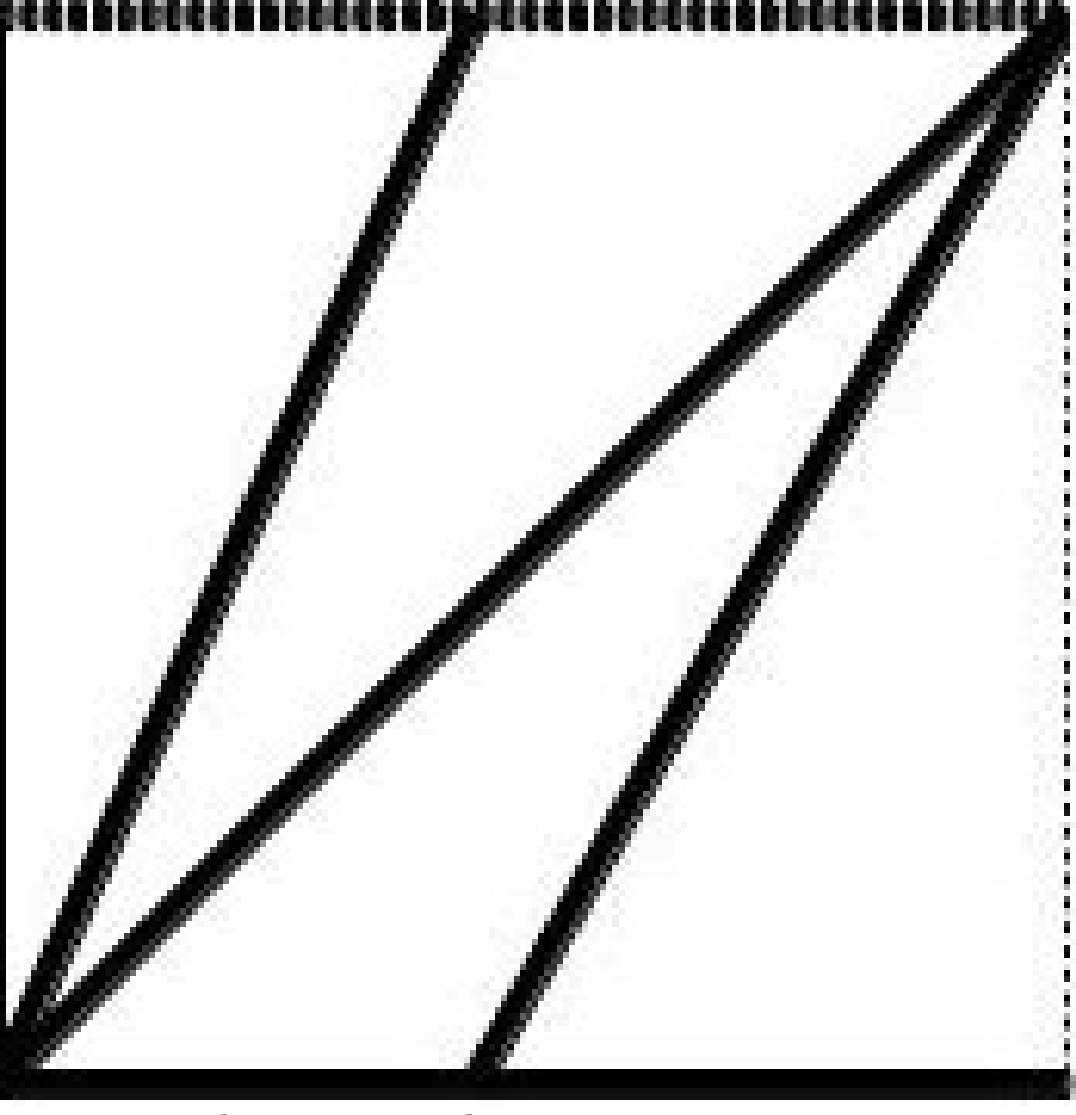
\includegraphics[width=0.42\linewidth]{fig6-1.png}
  \caption{粗线标出三个拉格朗日子流形，虚线表示周期性重复。\origloc{原文 Figure 6.1，第 24 页}}
  \label{fig:6-1}
\end{figure}

在 B 侧，这些对象将对应于线丛 $\mathcal{L}_0=\mathcal{O}$、$\mathcal{L}_1=\mathcal{L}_{\varphi_0}$ 与 $\mathcal{L}_2=\mathcal{L}_{\varphi_0}^2$。注意 $\mathcal{L}_{\varphi_0}:=\mathcal{L}(\varphi_0)$ 是我们上面定义的特殊选取的 $1$ 次线丛。

于是我们希望我们的函子把
\[
  \mathbb{C}^{|L_i\cap L_j|}=\operatorname{Hom}(\mathcal{L}_i,\mathcal{L}_j)
  \ \longrightarrow\ \operatorname{Hom}(\mathcal{L}_i,\mathcal{L}_j)
  =H^0(\mathcal{L}_j\otimes\mathcal{L}_i^*)
\]
以与复合相容的方式送出。

观察：
\[
\begin{aligned}
\operatorname{Hom}(\mathcal{L}_0,\mathcal{L}_1)&\cong H^0(\mathcal{L}_{\varphi_0})
  =\operatorname{span}_{\mathbb{C}}\bigl(\{\theta_\tau(z)\}\bigr),\\
\operatorname{Hom}(\mathcal{L}_1,\mathcal{L}_2)&\cong H^0(\mathcal{L}_{\varphi_0})
  =\operatorname{span}_{\mathbb{C}}\bigl(\{\theta_\tau(z)\}\bigr),\\
\operatorname{Hom}(\mathcal{L}_0,\mathcal{L}_2)&\cong H^0(\mathcal{L}_{\varphi_0}^2)
  =\operatorname{span}_{\mathbb{C}}\bigl(\{\theta[0,0](2\tau,2z),\ \theta[1/2,0](2\tau,2z)\}\bigr).
\end{aligned}
\]

态射的复合由逐纤维乘法给出。因此，上面的加法公式 4.3 决定了这个简单例子在 A 侧的所有复合。

让我们来看 A 侧，找出我们的 $\mathfrak{m}_2$ 复合算子。由图 6.1 可见
\[
  L_0\cap L_1=\{e_1\},\qquad L_1\cap L_2=\{e_1\},\qquad L_0\cap L_2=\{e_1,e_2\}.
\]
回想上面的提升引理（以及注 5.7）。把 $e_1$ 的提升固定为 $\mathbb{C}$ 中的原点，则我们的三角形由映到 $L_1$ 的边界段的绕数（包括定向\footnote{这是相对于 $L_1$ 由其分级（即 $\alpha$ 的选取）所获得的定向而言。}）决定。

注意，当浸入 $\gamma_1\looparrowright L_1$ 的绕数为偶数时，三角形的所有顶点都下降到 $E_\tau$ 中的同一个点。在奇数情形，$e_2=\pi(1/2)$。这些三角形的面积\footnote{在本例中 B-场平凡，$\phi^*\omega_{\mathbb{C}}$ 给出提升圆盘的面积；但一般而言这一量将是复数，通常称为 $\phi$ 的能量。}分别为 $\phi^*\omega_{\mathbb{C}}=\tau n^2=iAn^2$ 与 $\phi^*\omega_{\mathbb{C}}=\tau(n+\tfrac12)^2=iA(n+\tfrac12)^2$（原文如此，原文第二个等式左端误作 $\tau n^2$），其中 $n$ 是 $\gamma_1\looparrowright L_1$ 的绕数。

于是
\[
  \mathfrak{m}_2(e_1,e_1)=C(e_1,e_1,e_1)\cdot e_1+C(e_1,e_1,e_2)\cdot e_2,
\]
其中
\[
  C(e_1,e_1,e_1)=\sum_{n\in\mathbb{Z}}e^{-2\pi An^2},
  \qquad
  C(e_1,e_1,e_2)=\sum_{n\in\mathbb{Z}}e^{-2\pi A(n+1/2)^2}.
\]
注意 $C(e_1,e_1,e_1)=\theta[0,0](2iA,0)=\theta_{2\tau}(0)$，而 $C(e_1,e_1,e_2)=\theta[1/2,0](2\tau,0)$（原文如此，原文此处误作 $\theta[1/2,0](\tau,0)$，漏写因子 $2$）。

% [Tutor Note: 易错点 —— $\mathfrak{m}_2$ 的系数来自圆盘计数 $\sum_{[\phi]}e^{2\pi i\int_\phi\phi^*\omega_{\mathbb{C}}}$（5.5 节），其中 $\omega_{\mathbb{C}}=B+i\omega$。本例 $B=0$，$\int_\phi\phi^*\omega_{\mathbb{C}}=iAn^2$，故权重为 $e^{2\pi i\cdot iAn^2}=e^{-2\pi An^2}$；若 $B\neq0$ 还应再乘 $e^{2\pi iBn^2}$（关于 $n$ 是二次的）。而本节末“非平凡联络”一段出现的 $e^{2\pi in\beta}$ 关于 $n$ 是线性的，它来自绕 $L_2$ 一周的平行移动（单值），不是 B-场项，两者不要混淆。另注意 $\theta[a,b]$ 中 $b$ 的相位约定为 $e^{2\pi i(m+a)b}$（4.1 节），若改用 $e^{\pi i(\cdots)}$ 的约定则 $b$ 的因子差 $2$。]

于是 $\mathfrak{m}_2(e_1\otimes e_1)=\theta_{2\tau}(0)\cdot\theta_{2\tau}(2z)+\theta[1/2,0](2\tau,0)\cdot\theta[1/2,0](2\tau,2z)\in H^0(\mathcal{L}_{\varphi_0}^2)=\operatorname{Hom}(\mathcal{L}_0,\mathcal{L}_2)$（原文如此，原文左端误作 $\mathfrak{m}_2(e_1\otimes e_2)$）。
事实上，由上面的加法公式，$\mathfrak{m}_2(e_1\otimes e_1)=[\theta_\tau(z)]^2$。

这表明我们的函子也许把
\[
\begin{aligned}
\operatorname{Hom}(\mathcal{L}_0,\mathcal{L}_1)&\to\operatorname{Hom}(\mathcal{L}_0,\mathcal{L}_1),
  & e_1&\mapsto\theta_\tau(z),\\
\operatorname{Hom}(\mathcal{L}_1,\mathcal{L}_2)&\to\operatorname{Hom}(\mathcal{L}_1,\mathcal{L}_2),
  & e_1&\mapsto\theta_\tau(z),\\
\operatorname{Hom}(\mathcal{L}_0,\mathcal{L}_2)&\to\operatorname{Hom}(\mathcal{L}_0,\mathcal{L}_2),
  & e_1&\mapsto\theta[0,0](2\tau,2z),\\
&& e_2&\mapsto\theta[1/2,0](2\tau,2z).
\end{aligned}
\]
送出。

% [Tutor Note: 原文勘误 —— 第 25–27 页：（i）“From figure 6” 应为 “Figure 6.1”，译文径改（图中粗线确为三条测地线）；（ii）两处面积公式的第二式左端原作 $\tau n^2$，按右端 $iA(n+1/2)^2=\tau(n+1/2)^2$ 应为 $\tau(n+1/2)^2$，译文已订正并在正文括注；（iii）$C(e_1,e_1,e_2)$ 的识别式原作 $\theta[1/2,0](\tau,0)$，应按 $\sum_n e^{-2\pi A(n+1/2)^2}$ 与 $\theta[a,0]$ 的定义改为 $\theta[1/2,0](2\tau,0)$，原文漏写因子 $2$，译文已订正；（iv）$\mathfrak{m}_2(e_1\otimes e_2)=\theta_{2\tau}(0)\theta_{2\tau}(2z)+\cdots$ 的左端应为 $\mathfrak{m}_2(e_1\otimes e_1)$（与上一行 $\mathfrak{m}_2(e_1,e_1)$ 的展开以及紧随的 $\mathfrak{m}_2(e_1\otimes e_1)=[\theta_\tau(z)]^2$ 一致），译文已订正；（v）第 23 页 “our functor takes gives”、第 24 页 “lets assume” 均为笔误，译文径改。]

现在让我们把这个简单例子稍微复杂化一点，看看在 A 侧用另一条斜率 $2$ 的测地线替换 $L_2$ 时会发生什么。设 $L_2$ 是 $E^\tau$ 中由斜率为 $2$、$x$ 截距为 $x_0\in(0,1/2)$ 的直线下降得到的测地线。\footnote{不失一般性，可设 $x_0\in(0,1/2)$。}用 $\mathcal{L}'_2$ 记相应的带平凡联络的局部系统。

\begin{figure}[htbp]
  \centering
  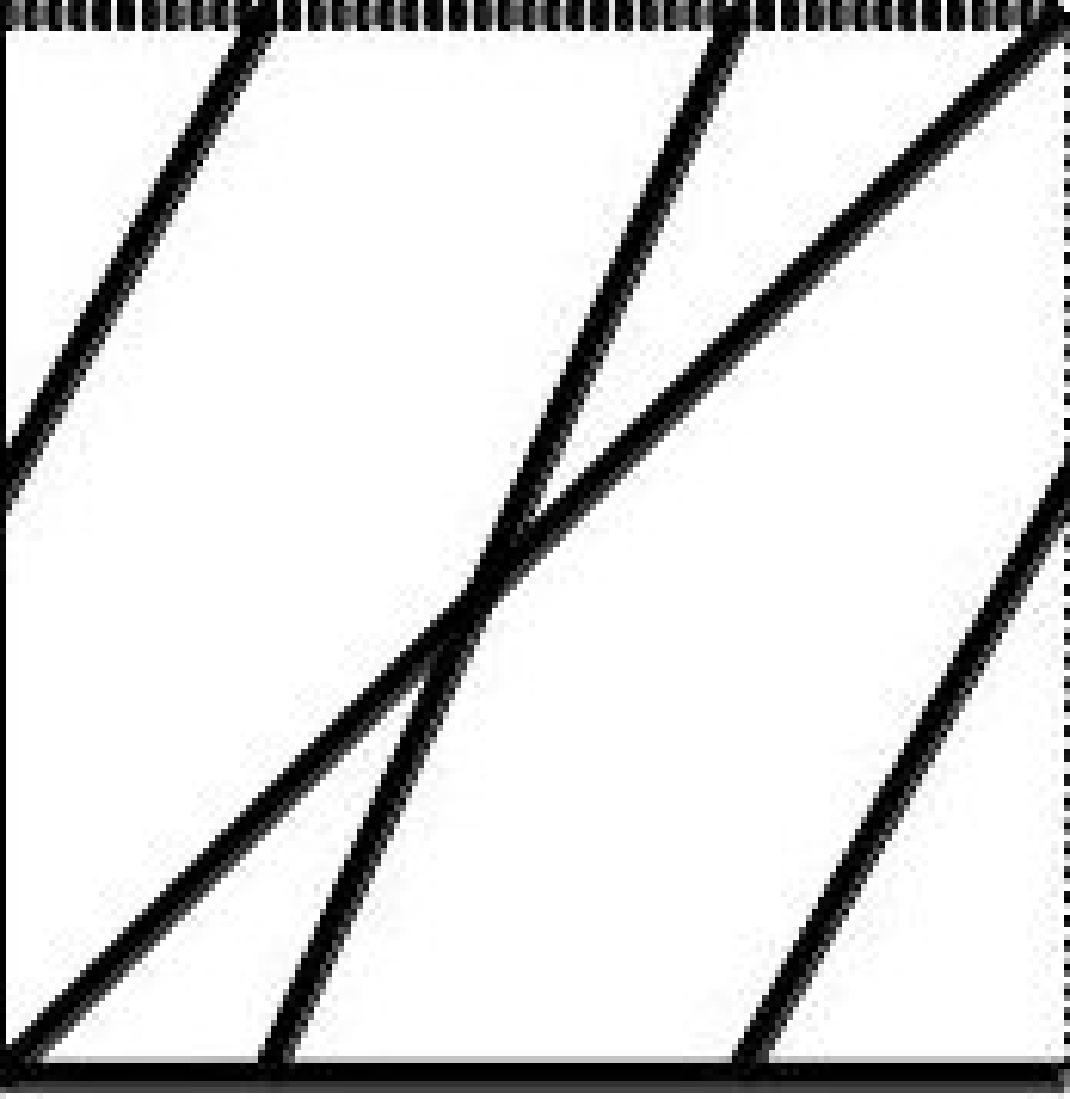
\includegraphics[width=0.42\linewidth]{fig6-2.png}
  \caption{平移情形。\origloc{原文 Figure 6.2，第 26 页}}
  \label{fig:6-2}
\end{figure}

现在我们有
\[
  \mathfrak{m}_2(e_1\otimes e'_2)=C(e_1,e'_2,p_1)\cdot p_1+C(e_1,e'_2,p_2)\cdot p_2,
\]
其中
\[
  C(e_1,e'_2,p_1)=\sum_{n\in\mathbb{Z}}e^{-2\pi A(n+x_0)^2}=\theta[x_0,0](2\tau,0),
\]
\[
  C(e_1,e'_2,p_2)=\sum_{n\in\mathbb{Z}}e^{-2\pi A(n+1/2-x_0)^2}
  =\sum_{n\in\mathbb{Z}}e^{-2\pi A(n+x_0+1/2)^2}=\theta[1/2+x_0,0](2\tau,0).
\]
注意 $\theta[1/2-x_0,0](2\tau,0)=\theta[1/2+x_0,0](2\tau,0)$。

按照上面的函子，$\mathcal{L}'_2$ 的镜像应当是 $t^*_{x_0\tau}\mathcal{L}_{\varphi_0}^2$。于是在这种情况下我们有
\[
\begin{aligned}
\operatorname{Hom}(\mathcal{L}_0,\mathcal{L}_1)&=\operatorname{span}_{\mathbb{C}}\{\theta_\tau(z)\},\\
\operatorname{Hom}(\mathcal{L}_1,\mathcal{L}'_2)&=H^0(t^*_{2x_0\tau}\mathcal{L}_{\varphi_0})
  =\operatorname{span}_{\mathbb{C}}\{t^*_{2x_0\tau}\theta_\tau(z)\}.
\end{aligned}
\]

因此我们的复合 $\mathcal{L}_0\to\mathcal{L}_1\to\mathcal{L}'_2$ 由乘积 $\theta_\tau(z)\cdot\theta_\tau(z+2x_0\tau)$ 决定，并且应当属于空间
\[
  \operatorname{Hom}(\mathcal{L}_0,\mathcal{L}'_2)
  =H^0(t^*_{x_0\tau}\mathcal{L}_{\varphi_0}^2)
  =\operatorname{span}_{\mathbb{C}}\{\theta[j/2,2x_0\tau](2\tau,2z)\}_{j\in\mathbb{Z}/2\mathbb{Z}}
\]
（原文如此，原文下标误作 $j\in\mathbb{Z}/j\mathbb{Z}$）。由上面的 $\theta$ 函数加法公式，我们有
\[
\begin{aligned}
&\theta_\tau(z)\cdot\theta_\tau(z+2x_0\tau)\\
&\quad=\theta_{2\tau}(2x_0\tau)\theta_{2\tau}(2z+2x_0\tau)
  +\theta[1/2,0](2\tau,2x_0\tau)\theta[1/2,0](2\tau,2z+2x_0\tau)\\
&\quad=e^{-2\pi ix_0^2\tau}\Bigl[\theta[x_0,0](2\tau,0)\theta[0,2x_0\tau](2\tau,2z)
  +\theta[x_0+1/2,0](2\tau,0)\theta[1/2,2x_0\tau](2\tau,2z)\Bigr].
\end{aligned}
\]
这告诉我们，我们的函子通过如下方式保持复合：
\[
\begin{aligned}
\operatorname{Hom}(\mathcal{L}_0,\mathcal{L}'_2)&\to\operatorname{Hom}(\mathcal{L}_0,\mathcal{L}'_2),\\
p_1&\mapsto\theta[0,0](2\tau,2z),\\
p_2&\mapsto\theta[1/2,0](2\tau,2z).
\end{aligned}
\]
（原文如此，原文把两端的 $\mathcal{L}'_2$ 都写成 $\mathcal{L}_2$。）

% [Tutor Note: 原文勘误 —— 第 26–27 页：（i）平移情形下函子两处写作 $\operatorname{Hom}(\mathcal{L}_0,\mathcal{L}_2)\to\operatorname{Hom}(\mathcal{L}_0,\mathcal{L}_2)$，按上下文应为 $\mathcal{L}'_2$，译文已订正并在正文括注；（ii）$\operatorname{Hom}(\mathcal{L}_0,\mathcal{L}'_2)$ 的基下标原作 $j\in\mathbb{Z}/j\mathbb{Z}$，遍历的应为 $\mathbb{Z}/2\mathbb{Z}$，译文已订正；（iii）第 27 页 “for $t_2$ some coordinate on $L_2$ with $t_2+1\ t_2$” 中 $1$ 与 $t_2$ 之间漏排 “$\sim$”，按上下文应为 $t_2+1\sim t_2$，译文已补；（iv）交点记号在未平移情形用 $e_1,e_2$、在平移情形用 $p_1,p_2$，原文交替使用，译文照原文保留。]

在离开这个简单例子之前，让我们看看当给 $\mathcal{L}_2$ 一个非平凡联络时会发生什么。设 $\nabla_2=\mathrm{d}+2\pi i\beta\,\mathrm{d}t_2$，其中 $t_2$ 是 $L_2$ 上的某个坐标，满足 $t_2+1\sim t_2$（原文如此，原文漏排 “$\sim$”）。于是
\[
  C(e_1,e_1,e_1)=\sum_{n\in\mathbb{Z}}e^{-2\pi An^2+2\pi in\beta}=\theta[x_0,\beta](2\tau,0),
\]
\[
  C(e_1,e_1,e_2)=\sum_{n\in\mathbb{Z}}e^{-2\pi A(n+1/2)^2+2\pi i(n+1/2)\beta}
  =\theta[x_0+1/2,\beta](2\tau,0).
\]
我们再次用等式 4.1 求出 B 侧的乘积；这一次 $x=2x_0\tau+\beta$。留给读者作为练习去验证：在这种情况下复合仍被保持。

\section{B 侧}

\begin{keytakeaways}
\begin{itemize}[leftmargin=1.6em,itemsep=1pt,topsep=2pt]
  \item \textbf{几何图像：}B 侧即复几何一侧：椭圆曲线 $E_\tau$ 上凝聚层的有界导出范畴 $\mathcal{D}^b(E_\tau)$，其对象是不可分解全纯向量丛与单点挠层的平移直和。
  \item \textbf{数学工具：}导出范畴的局部化（对拟同构形式地取逆）、$\operatorname{Ext}$ 群与 Serre 对偶、阿蒂亚（Atiyah）对椭圆曲线上全纯向量丛的分类、以 $\theta$ 函数为 $H^0$ 的基。
  \item \textbf{关键结论：}定理 7.6 把每个不可分解全纯向量丛写成 $\pi_{r*}(\mathcal{L}_{q^r}(\varphi)\otimes F_{q^r}(V,\exp N))$；引理 7.7 则给出 $H^0(\mathcal{L}(\varphi))\otimes V\cong H^0(\mathcal{L}(\varphi)\otimes F(V,\exp N))$ 的典范同构 (7.1)，从而使 B 侧的态射集仍可用 $\theta$ 基来计算。
  \item \textbf{后文接口：}本节对 $\mathcal{D}^b(E_\tau)$ 的“生成元 + 对偶 + 分类”描述，是第 8 节构造 A、B 两侧等价函子的直接依据。
\end{itemize}
\end{keytakeaways}

\subsection{凝聚层的导出范畴}

设 $\mathcal{A}$ 是某个阿贝尔范畴，并考虑 $\mathcal{A}$ 中链复形的范畴 $\mathcal{C}\mathcal{A}$，其对象是（$\mathcal{A}$ 中对象的）链复形，态射是链映射。\footnote{注意，所谓“有界”，指的是满足如下条件的复形 $A^\bullet$：当 $n\gg0$ 时 $A^n=0$。此外，在定义 $\mathcal{D}^b\mathrm{Coh}(X)$ 时，我们严格说来用的是上链复形。}$\mathcal{A}$ 的同伦范畴记作 $\mathcal{H}\mathcal{A}$，它与 $\mathcal{A}$ 有相同的对象，但把态射视为同伦等价的。$\mathcal{A}$ 的导出范畴 $\mathcal{D}\mathcal{A}$，是 $\mathcal{H}\mathcal{A}$ 对拟同构的局部化（即我们形式地为拟同构添加逆态射）。在镜像对称中，我们谈论的总是某个簇 $X$ 上凝聚层的有界导出范畴 $\mathcal{D}^b\mathrm{Coh}(X)$（或者，像我们这里将做的那样，简记为 $\mathcal{D}^b(X)$）。它是 $\mathcal{D}\mathcal{A}$ 的满子范畴，由 $\mathrm{Coh}_X(\mathcal{A})$ 中长度有限的链复形组成。这些概念在第 A.2 节有更详细的解释；但对这里所关心的情形 $\mathcal{D}^b(E_\tau)$ 而言，几乎不需要理解这一般理论。本节将收集关于 $\mathcal{D}^b(X)$ 与 $X$ 上凝聚层的一些标准事实，用它们来得到 $\mathcal{D}^b(E_\tau)$ 的一个简单描述。本节的所有结果要么是标准的，要么已在 [37, 31] 中证明。

% [Tutor Note: 易错点 —— “导出范畴”是 $\mathcal{H}\mathcal{A}$ 对拟同构作局部化（形式添加逆态射）得到的，不是普通商范畴；故 $\mathcal{D}^b(X)$ 的态射须用“屋顶”（左分式）表示，直接写链映射并不合法，参见附录 A.2 与 [28]。另，原文 “chain complexes in $\mathrm{Coh}_X(\mathcal{A})$ of finite length” 中的 $\mathrm{Coh}_X(\mathcal{A})$ 疑为 $\mathrm{Coh}(X)$ 之误（$\mathcal{A}$ 已被取为凝聚层范畴），译文照原文排印，未作改动。]

凝聚层的经典例子是向量丛的局部截面空间。这一对应给出局部自由凝聚层与流形上向量丛之间的一个自然等价。有鉴于此，我们常会（在语言上稍作滥用地）把一个（局部自由的）凝聚层称为向量丛，或反过来。为了（在椭圆曲线这一简单情形中）避开不必要的代数几何，我们以下述定理代替凝聚层的定义。

\begin{theorem}
黎曼曲面上的所有不可分解\footnote{一个层（或向量丛）$X$ 称为不可分解的，若 $X\cong X_1\oplus X_2\Rightarrow X_1\cong0$ 或 $X_2\cong0$。}凝聚层，要么是不可分解的向量丛，要么是支在单点的挠层。
\end{theorem}

\begin{proof}
参见 [37] 或 [19, Ex. III.6.11]。
\end{proof}

\begin{remark}
$E_\tau$ 上支在单点 $\zeta_0\in E_\tau$ 的挠层 $\mathcal{F}$，由有限维（复）向量空间 $V:=\mathcal{F}_{\zeta_0}$ 与一个幂零自同态 $N\in\operatorname{End}(V)$ 决定。沿用 [37, 31]，我们把这样的层记作 $S_\tau(\zeta_0,V,N)$。换言之，
\[
  S_\tau(\zeta_0,V,N):=\mathcal{O}_{r\zeta_0}\otimes V\big/\bigl\langle
  \zeta-\zeta_0-\frac{1}{2\pi i}N\bigr\rangle,
\]
其中 $\mathcal{O}_{r\zeta_0}$ 由正合列
\[
  \mathcal{O}\xrightarrow{(\zeta-\zeta_0)^r}\mathcal{O}\to\mathcal{O}_{r\zeta_0}
\]
定义。

$S_\tau(\zeta_0,V,N)$ 不可分解，当且仅当 $N$ 的核是一维的（因为这将推出 $N^r=0$ 而 $N^{r-1}\neq0$，其中 $r=\dim(V)$）。
\end{remark}

% [Tutor Note: 等价性的要点 —— 对幂零 $N$，“$\dim\ker N=1$” 等价于“$N$ 只有一个 Jordan 块”，即存在 $r=\dim V$ 使 $N^r=0$、$N^{r-1}\neq0$；这正是 $S_\tau(\zeta_0,V,N)$ 不可分解的充要条件。原文仅以一句 “as this implies $N^r=0$ and $N^{r-1}\neq0$” 带过，读者可用 Jordan 标准形自行补足（并与引理 7.7 中“核为一维”的假设对照）。]

对 $\mathcal{D}^b(C)$ 中的对象 $\mathcal{F}$，以 $\mathcal{F}[-n]$ 记除第 $n$ 次项为 $\mathcal{F}$ 之外全由零对象组成的链复形。\footnote{我们常滥用记号，把 $\mathcal{F}[0]$ 记作 $\mathcal{F}$。此外，若 $\mathcal{F}$ 已是某个复形范畴中的链，我们仍用 $\mathcal{F}[-n]$ 记相应的平移链。}

\begin{theorem}[{[31]}]
设 $C$ 是紧黎曼曲面。对象 $\mathcal{F}[n]$ 的有限直和（其中 $\mathcal{F}$ 是 $C$ 上的不可分解凝聚层）构成 $\mathcal{D}^b(C)$ 的一个满子范畴，且该子范畴等价于 $\mathcal{D}^b(C)$。
\end{theorem}

我们可以如下陈述 B 侧的 Serre 对偶（证明见 [31]）。

\begin{lemma}
设 $\mathcal{F}$ 与 $\mathcal{G}$ 是 $E_\tau$ 上的两个凝聚层，则存在函子性同构 $\operatorname{Hom}(\mathcal{F},\mathcal{G})\cong\operatorname{Ext}^1(\mathcal{G},\mathcal{F})^*$。
\end{lemma}

对任意阿贝尔范畴中的任意对象 $A,B$，我们有\footnote{这常被取作定义；解释见 [28] 或 [18, 第 I.6 节]。}
\[
  \operatorname{Hom}_{\mathcal{D}\mathcal{A}}(A[m],A[n])
  \cong\operatorname{Hom}_{\mathcal{D}\mathcal{A}}(A,B[m-n])
  \cong\operatorname{Ext}^{m-n}(A,B).
\]

% [Tutor Note: 原文勘误 —— （i）引理 7.4 原文作 “Let $\mathcal{F}$ and $\mathcal{G}$ be \emph{to} coherent sheaves”，应为 “be two coherent sheaves”，译文径改；（ii）紧接的通用公式原文左端第二个对象作 $A[n]$，而同式其余部分用 $B$，且移位方向亦不自洽；按标准约定 $\operatorname{Hom}(X[m],Y[n])=\operatorname{Hom}(X,Y[n-m])\cong\operatorname{Ext}^{n-m}(X,Y)$，全式应统一为 $B[n]$ 与 $n-m$。此处疑为原文笔误，译文照原文排印，请核对 [28] 或 [18, I.6]。]

令我们的阿贝尔范畴为 $E_\tau$ 上的凝聚层，并利用上述引理，就得到函子性同构
\[
  \operatorname{Hom}_{\mathcal{D}^b(E_\tau)}(A,B[1])=\operatorname{Ext}^1(A,B)=\operatorname{Hom}(B,A)^*,
\]
\[
  \operatorname{Hom}_{\mathcal{D}^b(E_\tau)}(A,B)=\operatorname{Ext}^0(A,B):=\operatorname{Hom}(A,B).
\]

\begin{lemma}
对黎曼曲面上的凝聚层 $A,B$，除 $k\in\{0,1\}$ 外 $\operatorname{Ext}^k(A,B)=0$。
\end{lemma}

\begin{proof}
一般地，对复 $n$ 维流形，$\operatorname{Ext}^k$ 函子在 $k>n$ 时消没。参见 [19, Ex. III.6.5]。
\end{proof}

% [Tutor Note: 省略证明 —— 定理 7.3（$\mathcal{D}^b(C)$ 由不可分解凝聚层的移位 $\mathcal{F}[n]$ 的有限直和生成）与引理 7.5（$\operatorname{Ext}^k=0\ (k>1)$）在原文中都只给出文献出处：前者见 [31]，后者是复 $n$ 维流形上 $\operatorname{Ext}^k$ 对 $k>n$ 消没的特例（[19, Ex. III.6.5]）。另，引理 7.5 原文把指标集印作 “$k\in0,1$”（漏排花括号），译文按 $\{0,1\}$ 排印。]

我们将在第 8 节讨论 Serre 对偶的镜像。

\subsection{$E_\tau$ 上全纯向量丛的分类}

设 $V$ 为有限维（复）向量空间，并考虑 $E_q$ 上由
\[
  F_q(V,A)=\mathbb{C}^*\times V/(u,v)\sim(uq,A\cdot v)
\]
给出的全纯向量丛，其中 $A\in\operatorname{GL}(V)$。

由于 $\mathbb{C}^*$ 上的全纯向量丛都是平凡的，4.2 节中的相关论证仍然成立：我们可以用这种方式描述所有线丛（唯一到满足 $A(u)=B(qu)A(u)B(u)^{-1}$ 的 $B:\mathbb{C}^*\to\operatorname{GL}(V)$ 为止）。

若 $A=\exp(N)$，其中 $N$ 是核为一维的幂零自同态\footnote{$\exp(N)$ 总是可逆的，因为 $\det(e^N)=e^{\operatorname{Tr}(N)}$。}，则 $F_q(V,\exp(N))$ 不可分解。此外，我们有阿蒂亚（Atiyah）[1] 给出的如下分类（定理 7.6）。

考虑 $r$ 重覆叠 $\pi_r:E_{q^r}\to E_q$。$\pi_r$ 通过其拉回与前推定义一个函子，而该函子将与我们的镜像函子交换（我们将在后文更详细地讨论这个函子及其镜像，见第 8.1 节）。

\begin{theorem}
$E_\tau$ 上的每个不可分解全纯向量丛都形如
\[
  \pi_{r*}\bigl(\mathcal{L}_{q^r}(\varphi)\otimes F_{q^r}(V,\exp(N))\bigr),
\]
其中 $\varphi$ 是某个（$\mathbb{C}^*\to\mathbb{C}^*$ 的）全纯函数，$N$ 是某个核为一维的幂零自同态。
\end{theorem}

% [Tutor Note: 省略证明 —— 定理 7.6 是 Atiyah 对椭圆曲线上全纯向量丛的分类（[1]，另见 [37, 第 2 节] 与 [31]）的改写，原文未给证明。其次，作者称 $\pi_r$ 的拉回与前推“将与我们的镜像函子交换”，其函子性（$\pi_{r*}$ 与 $\pi_r^*$ 的伴随关系，以及与 $t^*_x$、张量积的相容性）也未展开，细节见 [37, 31]。另注意原文在 $E_\tau$ 与 $E_q$（4.2 节的参数化 $\mathbb{C}^*/u\sim qu$）两种记号之间切换，且定理中同一对象上同时出现 $\mathcal{L}_{q^r}$（线丛）与 $F_{q^r}$（向量丛）。另，第 29 页的 “an finite”“homomorphic”“functorality”“can be again be dealt with” 以及一处括号不配对均为原文笔误，译文径改。]

在下一节中，我们将在 A 侧形式上添加双积；因此在定义我们的函子（以及加性范畴的等价）时，只需在这些不可分解丛上定义它就够了。此外，我们将有：该等价与 $\pi_*$ 交换，于是只需考虑形如 $\mathcal{L}(\varphi)\otimes F(V,\exp(N))$ 的对象。一旦 $\pi_*$ 的函子性被明确建立，下面的命题就告诉我们，我们的态射集又可以借助 $\theta$ 函数的基（系数为常向量）来处理。

\begin{lemma}
设 $\varphi=(t^*_x\varphi_0)\cdot\varphi_0^{n-1}$，对某个 $n>0$。则对任意幂零 $N\in\operatorname{End}(V)$，存在典范同构
\begin{equation}\tag{7.1}
  \Psi_{\varphi,N}:=H^0(\mathcal{L}(\varphi))\otimes V
  \xrightarrow{\ \sim\ }
  H^0(\mathcal{L}(\varphi)\otimes F(V,\exp(N)))
\end{equation}
\begin{equation}\tag{7.2}
  f\otimes v\mapsto\exp(DN/n)f\cdot v
\end{equation}
其中 $D=-u\frac{\mathrm{d}}{\mathrm{d}u}=-\frac{1}{2\pi i}\frac{\mathrm{d}}{\mathrm{d}z}$。
\end{lemma}

\begin{proof}
这很容易验证。参见 [37]。
\end{proof}

% [Tutor Note: 关于引理 7.7 与第 30 页 Hom 计算 —— (a) 易错点：算子 $D=-u\frac{\mathrm{d}}{\mathrm{d}u}=-\frac{1}{2\pi i}\frac{\mathrm{d}}{\mathrm{d}z}$ 的第二个等号依赖 $u=e^{2\pi iz}$（4.1 节中 $q=e^{2\pi i\tau}$，$u$ 为 $\mathbb{C}^*$ 上的坐标）；若把 $u$ 取作 $e^{-2\pi iz}$，则 $D$ 与 $\exp(DN/n)$ 的相位整体反号。(b) 省略证明：$\exp(DN/n)$ 是作用在 $\theta$ 函数上的有限和（因 $N$ 幂零），故 (7.2) 右端确实落在 $H^0(\mathcal{L}(\varphi)\otimes F(V,\exp(N)))$ 中；原文 “This is simple to check” 一句省略了对 $\mathcal{L}(\varphi)$ 的转移函数与 $F(V,\exp(N))$ 的拼接矩阵相容性的验证，细节见 [37]。(c) 原文勘误：第 30 页 “using lemma 7.1” 按上下文应为“引理 7.7”（$\varphi_i$ 的分解式正来自引理 7.7），译文已订正并在正文括注。又，$\operatorname{Hom}(\mathcal{V}_1,\mathcal{V}_2)$ 的计算用到 $\mathcal{L}(\varphi)^*=\mathcal{L}(\varphi^{-1})$、$\operatorname{Hom}(V_1,V_2)=V_1^*\otimes V_2$ 以及 $F(V_1,A_1)^*\otimes F(V_2,A_2)=F(V_1^*\otimes V_2,(A_1^{-1})^*\otimes A_2)$；末行 $F(V,A)^*=F(V^*,(A^{-1})^*)\cong F(V,A^{-1})$ 的第二个同构默认了 $V\cong V^*$ 的（非典范）同构，核对时以第一个等式为准。]

考虑两个向量丛 $\mathcal{V}_i=\mathcal{L}(\varphi_i)\otimes F(V_i,\exp(N_i))$，其中 $\varphi_i=(t^*_{x_i}\varphi_0)\cdot\varphi_0^{n_i-1}$ 且 $n_1<n_2$；利用引理 7.7（原文如此，原文误作引理 7.1），我们便有
\[
\begin{aligned}
\operatorname{Hom}(\mathcal{V}_1,\mathcal{V}_2)
&=H^0\bigl(\mathcal{L}(\varphi_1^{-1}\varphi_2)
  \otimes F(V_1^*\otimes V_2,\ \exp(\mathbf{1}\otimes N_2-N_1^*\otimes\mathbf{1}))\bigr)\\
&\cong H^0(\mathcal{L}(\varphi_1^{-1}\varphi_2))\otimes\operatorname{Hom}(V_1,V_2).
\end{aligned}
\]
注：$F(V,A)^*=F(V^*,(A^{-1})^*)\cong F(V,A^{-1})$。

% --- 译者交付说明：覆盖原文第 23–30 页（§6 全部与 §7 全部）；编号环境 8 个（remark 6.1；theorem 7.1、7.3、7.6；remark 7.2；lemma 7.4、7.5、7.7）；编号公式 (7.1)(7.2) 各一个 equation+tag；图 2 幅（fig6-1、fig6-2）；脚注 10 条（原文脚注 23 的文字在原 PDF 中缺失，仅保留编号占位；24–32 共 9 条为实译）；批注 12 条（§6 六条，§7.1 四条，§7.2 两条）。原文笔误清单（均已在正文或批注中说明）：(i) 第 23 页表格脚注 23 无脚注文字；(ii) 第 23 页 “takes gives”；(iii) 第 24 页 “lets assume”；(iv) 第 25 页 “From figure 6” 应为 figure 6.1；(v) 第 25 页面积公式第二式左端误作 $\tau n^2$；(vi) 第 25 页 $C(e_1,e_1,e_2)=\theta[1/2,0](\tau,0)$ 漏因子 2；(vii) 第 25 页 $\mathfrak{m}_2(e_1\otimes e_2)$ 应为 $\mathfrak{m}_2(e_1\otimes e_1)$；(viii) 第 26 页 $E^\tau$ 与 $E_\tau$ 混用；(ix) 第 26–27 页平移情形 Hom 中 $\mathcal{L}_2$ 应为 $\mathcal{L}'_2$；(x) 第 27 页基下标 $j\in\mathbb{Z}/j\mathbb{Z}$ 应为 $\mathbb{Z}/2\mathbb{Z}$；(xi) 第 27 页 $t_2+1\ t_2$ 漏排 $\sim$；(xii) 第 27—30 页 $e_i$ 与 $p_i$ 记号交替使用；(xiii) 第 28 页 “morphism are chain maps”“be to coherent sheaves”“by denote”“$\mathrm{Coh}_X(\mathcal{A})$” 以及 Hom(A[m],A[n]) 式中 $A[n]$/$B$ 与移位方向不一致；(xiv) 第 29 页 “an finite”“homomorphic”“functorality”“can be again be dealt with”、第 29 页括号不配对；(xv) 第 30 页 “using lemma 7.1” 应为引理 7.7。遗留问题：原文脚注 23 文字缺失待查原稿；A 侧辛环面 $E_\tau$/$E^\tau$ 与 B 侧 $E_\tau$、$E_q$ 的记号混用为原文所有，译文一律照排。 ---

% ===== 以下内容来自 sections/sec8.tex =====
% !TEX root = ../main.tex
% =============================================================================
%  §8 等价性（原文第 30–35 页）
%  Andrew A. Port, "An Introduction to Homological Mirror Symmetry and the
%  Case of Elliptic Curves", arXiv:1501.00730v1，§8，pp. 30–35
% =============================================================================

\section{等价性}

\begin{keytakeaways}
\begin{itemize}[leftmargin=1.6em,itemsep=1pt,topsep=2pt]
  \item \textbf{物理图像：}B 侧椭圆曲线 $E_\tau$ 上的 D-膜（凝聚层及其导出范畴）与 A 侧镜像椭圆曲线 $E^\tau$ 上的 D-膜（拉格朗日子流形连同局部系统）之间的对应；本节把这一物理陈述精确化为两个加性范畴的等价。
  \item \textbf{数学工具：}$A_\infty$-范畴的同调截断 $H^0$（只保留零次态射）、为补足双积而作的形式加性完备化（深谷–孔采维奇范畴）、阿蒂亚（Atiyah）向量丛分类、塞尔（Serre）对偶、覆叠映射的拉回/前推及其基变换。
  \item \textbf{镜像同源：}$r$ 重覆叠 $\pi_r$ 的镜像是同源 $p_r$；两侧的“拉回/前推”互换：$\Phi(\pi_{r*}A)=p_{r*}\Phi(A)$ 是把 $\Phi$ 从特殊丛延拓到所有不可分解丛的关键。
  \item \textbf{关键结论：}定理 8.4（主定理）断言 $\Phi_\tau:\mathcal{D}^b(E_\tau)\to\mathcal{FK}^0(E^\tau)$ 是保平移的加性范畴等价；这正是全篇要证明的目标。
  \item \textbf{显式公式：}本节给出 $\Phi_\tau$ 在对象上的公式（斜率 $n$、$y$ 截距 $-a$、单值 $e^{-2\pi ib}\exp(N)$）与在态射上的公式（相位因子 $e^{\pi i\delta_{21}^2(n_1-n_2)}$ 与矩阵指数 $\exp[\delta_{21}(N_2-N_1^*-2\pi i(n_2-n_1)\beta_{21})]$），使等价成为可以逐项验证的陈述。
\end{itemize}
\end{keytakeaways}

% [Tutor Note: 编号与字形 —— (1) 原文 §8 之下直接出现 “8.0.1.”（并无 8.0 小节），属编号遗留；译文按体例用不编号的 \subsection* 复现，故不进入目录。(2) 字形：原文在 \operatorname{Hom} 的变元处把拉格朗日对象印作花体 $\mathcal{L}$，而在 $(L,\alpha,M)$ 及几何语句（$p_r|_L$、$L\cap L'$）中印作斜体 $L$。本译本按全书体例统一：$\mathcal{L}$ 专指线丛，拉格朗日对象/子流形一律用斜体 $L$；若需严格照排原字形，可把这些 $L$ 改回 $\mathcal{L}$。]

\subsection*{8.0.1\quad 深谷–孔采维奇范畴}

[37, 31] 中证明的等价并不是 $A_\infty$-范畴的等价，而是加性范畴 $\mathcal{D}^b(E_\tau)$ 与 $\mathcal{FK}^0(E^\tau):=H^0(\mathrm{Fuk}(E^\tau))$ 之间的等价。\footnote{注意，我们只在 $k+1$ 个互不相同的拉格朗日子流形的情形下定义了 $\mathfrak{m}_k$。[37, 36] 只处理这一情形，而 [31] 则通过直接构造 $\mathrm{Fuk}^0$，把 $k\ge 3$ 的高阶 $A_\infty$ 运算 $\mathfrak{m}_k$ 整个绕开了。一般情形下 $\mathfrak{m}_k$ 的定义由 [14, 15] 给出；但据作者所知，一般（非横截）情形下 $A_\infty$-（或三角）范畴之间等价性的证明尚未发表。不过，这一证明很可能被认为已经隐含在 [36, 14] 的联合工作之中。} 下面我们来解释这个 A 侧范畴指的是什么。

如我们先前所示（见注 5.7），$\mathrm{Fuk}(E^\tau)$ 上的微分算子为零。因此，其上同调复形与由按马斯洛夫–维特博（Maslov–Viterbo）指标 5.4 分次的态射集所给出的复形完全相同。首先，仿照 [37]，让我们下降/限制到平凡上同调，即 $\mathrm{Fuk}^0:=H^0(\mathrm{Fuk}(E^\tau))$：此时对象相同，但只考虑使 $\mu_{L,L'}=0$（即 $\alpha'-\alpha\in[0,1)$）的态射 $(L,\alpha,M)\to(L',\alpha',M')$。

上面我们只处理了横截的态射；在这种情形（$L\neq L'$）下，有\footnote{当上下文中清楚时，我们通常会从态射集中省略下标 $\mathrm{Fuk}^0$；B 侧亦然。}
\[
\operatorname{Hom}_{\mathrm{Fuk}^{0}(E^{\tau})}(L,L')
=\begin{cases}
0, & \text{若 } \alpha'-\alpha\notin[0,1),\\[2pt]
\displaystyle\bigoplus_{p\in L\cap L'}\operatorname{Hom}(M_p,M'_p), & \text{若 } \alpha'-\alpha\in[0,1).
\end{cases}
\]
当 $L=L'$ 时，有
\[
\operatorname{Hom}_{\mathrm{Fuk}^{0}(E^{\tau})}(L,L')
=\begin{cases}
0, & \text{若 } \alpha'-\alpha\notin[0,1),\\[2pt]
H^{0}\bigl(L,\operatorname{Hom}(M,M')\bigr)=\operatorname{Hom}(M,M'), & \text{若 } \alpha'=\alpha,\\[2pt]
H^{1}\bigl(L,\operatorname{Hom}(M,M')\bigr), & \text{若 } \alpha'=\alpha+1.
\end{cases}
\]
% [Tutor Note: 原文勘误与小笔误（第 30–31 页）—— (1) 第二个分段函数首行原文印作 “$\alpha'-\alpha\notin 0,1$”，漏排区间记号 $[\,)$；由上一式可知应为 $\alpha'-\alpha\notin[0,1)$，译文已补全。(2) 本段 “lets descend/restrict” 应为 “let us descend/restrict”。(3) 后文 “it additionally it has a zero object” 中 it 重复，译文按“进一步具有”处理。(4) 形式加性完备化的记号在下文印作带下划线的 $\underline{\mathcal{A}}$，PDF 文本层丢失了这条下划线，须按第 31 页图像还原。]

下降（取上同调）到 $H^0(\mathrm{Fuk})$ 后，我们得到一个真正的（即结合的）预加性范畴。\footnote{我们将忽略 $k\ge 3$ 的高阶 $A_\infty$ 运算 $\mathfrak{m}_k$，因为在这个弱化版的同调镜像对称中，我们并不寻求 $A_\infty$-范畴的等价。} 为了与 B 侧整个导出范畴建立等价，我们还必须考虑上述次数为一的态射（细节见 [31]）。

回忆在 $\mathrm{Fuk}^0(E^\tau)$ 中，$(L,\alpha,M)[1]:=(L,\alpha+1,M)$。

下面这个“辛塞尔对偶”（symplectic Serre duality）的证明同样可在 [31] 中找到。

\begin{lemma}
对 $\mathrm{Fuk}^0(E^\tau)$ 中的对象 $L_1,L_2$，存在典范同构
\[
\operatorname{Hom}(L_1,L_2[1])\cong\operatorname{Hom}(L_2,L_1)^{*}.
\]
\end{lemma}

$\mathrm{Fuk}^0(E^\tau)$ 不是加性范畴（按构造它只是预加性的\footnote{若一个范畴的每个态射集都是阿贝尔群、且态射的复合是双线性的，则称其为预加性范畴（或 Ab-范畴）。若它还进一步具有零对象并包含所有有限双积，则称为加性范畴。}）。若对某些非零对象 $L_k$ 存在（双积）$L=L_1\oplus L_2$，则我们有非零的投影与嵌入 $p_k:L\to L_k$ 以及 $i_k:L_k\to L$。这是不可能的（在拉格朗日子流形互不相同的情形下），因为我们已经限制到只有零次分次的态射，于是 $\operatorname{Hom}(L,L_1)$ 与 $\operatorname{Hom}(L_1,L)$ 不可能同时非平凡。这是一个问题，因为我们希望与加性范畴 $\mathcal{D}^b(E_\tau)$ 建立等价。[31] 通过把这些双积形式地添入来修正这一点。我们把这样形式地扩大的范畴称为\textit{深谷–孔采维奇（Fukaya–Kontsevich）范畴}，$\mathcal{FK}^0(E^\tau):=H^0(\mathrm{Fuk}(E^\tau))$。

设 $\mathcal{A}$ 是一个预加性范畴。我们定义 $\underline{\mathcal{A}}$ 为这样的范畴：其对象是 $\mathcal{A}$ 中对象的有序 $k$ 元组（$k\ge 0$），其态射是 $\mathcal{A}$ 中态射构成的矩阵；复合由矩阵乘法给出，零元组是零对象。

\subsection{镜像同源}

在我们构造 $\mathcal{D}^b(E_\tau)$ 与 $\mathcal{FK}^0(E^\tau)$ 之间的函子之前，需要先定义 $p_r:E^{r\tau}\to E^\tau$，即 $\pi_r$ 的镜像。

回忆 $\pi_r$ 是 $r$ 重覆叠 $E_{r\tau}\xrightarrow{\pi_r}E_\tau$。向量丛经 $\pi_r$ 的拉回由
\[
\pi_r^{*}F_q(V,A)\to F_{q^{r}}(V,A^{r})
\]
给出，其前推由
\[
\pi_{r*}F_{q^{r}}(V,A)=F_q(V^{\oplus r},\pi_*A)
\]
给出，其中 $\pi_*(A)\in\operatorname{GL}(V^{\oplus r})$ 把 $(v_1,\dots,v_r)$ 映为 $(v_2,\dots,v_r,Av_1)$。

这些函子在不可分解挠层
\[
S_\tau(\zeta_0,V,N):=\mathcal{O}_{r\zeta_0}\otimes V\Big/\Big\langle \zeta-\zeta_0-\frac{1}{2\pi i}N\Big\rangle
\]
上有类似的定义。

该函子的镜像 $p_r:E^\tau\to E^{r\tau}$ 由实平面的自同构 $(x,y)\mapsto(rx,y)$ 诱导（对任意正整数 $r$）。让我们考察 $p_r$ 到一个拉格朗日子流形 $L$ 上的限制。设 $L$ 的斜率为 $n/m$，其中 $\gcd(n,m)=1$。由于 $p_r$ 固定 $y$ 坐标，$p_r|_L$ 的次数为 $d=\gcd(n,r)$。\footnote{注意，在 $\gcd(n,m)=1$ 的假设下，$L$ 沿 $y$ 方向绕 $E^\tau$ 共 $n$ 圈。} 于是我们还必须有：一个（斜率为 $n/(rm)$ 的）拉格朗日子流形的原像有 $N=r/d=r/\gcd(n,r)$ 个连通分支。即 $p_r^{-1}(L)=\{L^{(1)},\dots,L^{(N)}\}$（稍后我们将用它来定义拉回）。

% [Tutor Note: 易错点（上下标与方向）—— 原文对 $p_r$ 的定向前后不一致：本小节开头印作 $p_r:E^{r\tau}\to E^\tau$，同段末又印作 $p_r:E^\tau\to E^{r\tau}$；第 32 页的 $p_{r*}:\mathcal{FK}^0(E^\tau)\to\mathcal{FK}^0(E^{r\tau})$ 与 $p_r^*:\mathcal{FK}^0(E^{r\tau})\to\mathcal{FK}^0(E^\tau)$ 也把两者颠倒了。按几何（$(x,y)\mapsto(rx,y)$ 把 $\mathbb{C}/\langle 1,r\tau\rangle$ 送到 $\mathbb{C}/\langle 1,\tau\rangle$）以及第 34 页的 $\Phi(\pi_{r*}A)=p_{r*}\Phi_{r\tau}(A)$ 和定理 7.6 中 $\pi_{r*}$ 的方向，正确的应是 $p_r:E^{r\tau}\to E^\tau$，$p_{r*}:\mathcal{FK}^0(E^{r\tau})\to\mathcal{FK}^0(E^\tau)$，$p_r^*:\mathcal{FK}^0(E^\tau)\to\mathcal{FK}^0(E^{r\tau})$。译文照页面图像排印，特此说明。又：次数 $d=\gcd(n,r)$ 与分支数 $N=r/d$ 的关系是——$p_r|_L$ 是 $d$ 重覆叠，故原像 $p_r^{-1}(L)$ 恰有 $N=r/d$ 个连通分支；这个 $N$ 正是下文拉回公式 $p_r^*(L,\alpha,M)=\bigoplus_{k=1}^{N}(\cdots)$ 中直和项数的来源。]

前推 $p_{r*}:\mathcal{FK}^0(E^\tau)\to\mathcal{FK}^0(E^{r\tau})$ 由
\[
p_{r*}(L,\alpha,M)\mapsto\bigl(p_r(L),\alpha',p_{r*}M\bigr)
\]
给出，其中 $p_{r*}:(v_1,\dots,v_d)\mapsto(v_2,\dots,v_d,Mv_1)$，而 $\alpha'$ 是 $\alpha$ 所在同一区间 $[k-1/2,k+1/2)$（对某个 $k\in\mathbb{Z}$）中唯一合适的取值。

函子性不难看出。
\begin{tikzcd}[column sep=5em, row sep=2.8em]
\operatorname{Hom}(L,L') \arrow[d,"p_{r*}"] & {}={} & \displaystyle\bigoplus_{\tilde{x}\in L\cap L'}\operatorname{Hom}(M_{\tilde{x}},M'_{\tilde{x}}) \arrow[d, hook] \\
\operatorname{Hom}(p_{r*}L,p_{r*}L') & {}={} & Z
\end{tikzcd}
其中
\[
Z:=\bigoplus_{x\in p_r(L)\cap p_r(L')}\operatorname{Hom}\Bigl(\ \bigoplus_{\tilde{x}\in(p_r|_{L})^{-1}(x)}M_{\tilde{x}},\ \bigoplus_{\tilde{x}'\in(p_r|_{L'})^{-1}(x)}M'_{\tilde{x}'}\Bigr).
\]

% [Tutor Note: 第 32 页的排印与文本层陷阱 —— (1) 上面的“同调图 + 直和”方块图按页面图像用 tikzcd 重排：左列为两行同调群，右列第一行为各分支交点的直和、第二行为 $Z$，右列自上而下的箭头为嵌入（hook，$\hookrightarrow$），中列为等号；原文用 $Z$ 表示第一行直和的“整体和”，故用嵌入箭头而非同构。(2) 紧随其后的那句 $\operatorname{Hom}(\pi_{r_1*}\mathcal{E}_1,\pi_{r_2*}\mathcal{E}_2))\to\operatorname{Hom}(p_{r_1*}\Phi(\mathcal{E}_1),p_{r_2*}\Phi(\mathcal{E}_2))$ 在原文中多印了一个右括号（“$\mathcal{E}_2))$”），译文已按数学含义订正为单括号。(3) PDF 文本层把命题 8.2 的两条公式都压成 “$\operatorname{Hom}(p^*L,L')\cong\operatorname{Hom}(L,p^*L')$”，看似重复；按第 32 页图像，第二条应为 $\operatorname{Hom}(p_*L,L')\cong\operatorname{Hom}(L,p^*L')$（$p_*$ 与 $p^*$ 位置互换），即第一条是 $p^*\dashv p_*$ 的伴随同构、第二条是 $p_*\dashv p^*$ 的伴随同构，二者并不重复。]

类似地，拉回 $p_r^*:\mathcal{FK}^0(E^{r\tau})\to\mathcal{FK}^0(E^\tau)$ 由
\[
p_r^{*}(L,\alpha,M)=\bigoplus_{k=1}^{N}\bigl(L^{(k)},\alpha',(p_r^{(k)})^{*}M\bigr)
\]
给出，其中 $p_r^{(k)}:=p_r|_{L^{(k)}}$，而 $(p_r^{(k)})^*M$ 是按通常方式拉回的局部系统。

下述 $p_r^*$ 与 $p_{r*}$ 之间的对偶的验证见 [31]。

\begin{proposition}
设 $p=t'_{n/m}\circ p_r$，其中 $n/m\in\mathbb{Q}$，且 $t'_\delta(x,y):=(x-\delta,y)$。则
\[
\operatorname{Hom}(p^{*}L,L')\cong\operatorname{Hom}(L,p_{*}L')
\]
以及
\[
\operatorname{Hom}(p_{*}L,L')\cong\operatorname{Hom}(L,p^{*}L').
\]
若把 $p$ 换为它的镜像 $\pi=t_{n\tau/m}\circ\pi_r$，则 B 侧亦有同样结论。
\end{proposition}

在按照定理 7.6 对凝聚层 $A=\mathcal{L}(\varphi)\otimes F(V,\exp(N))$ 定义好我们的镜像函子 $\Phi:\mathcal{D}^b(E_\tau)\to\mathcal{FK}^0(E^\tau)$ 之后，我们将通过证明
\[
\Phi(\pi_{r*}A)=p_{r*}\Phi(A)
\]
把 $\Phi$ 延拓到所有不可分解的丛上。

对于态射，我们需要知道如何把
\[
\operatorname{Hom}(\pi_{r_1*}\mathcal{E}_1,\pi_{r_2*}\mathcal{E}_2)\to\operatorname{Hom}(p_{r_1*}\Phi(\mathcal{E}_1),p_{r_2*}\Phi(\mathcal{E}_2))
\]
对应起来。

考虑 $\pi_{r_1}$ 与 $\pi_{r_2}$ 的范畴拉回 $E_{r_1\tau}\times_{E_\tau}E_{r_2\tau}:=\{(z_1,z_2)\mid\pi_{r_1}(z_1)=\pi_{r_2}(z_2)\}$。它是若干椭圆曲线的无交并；具体地，$E_{r_1\tau}\times_{E_\tau}E_{r_2\tau}=E_{r\tau}\times\mathbb{Z}_d$，其中 $d=\gcd(r_1,r_2)$，$r=\operatorname{lcm}(r_1,r_2)$。

% [Tutor Note: 记号提示 —— 原文用下标 $E_{r\tau}$ 表示 B 侧的 $r$ 重覆叠环面、用上标 $E^{r\tau}$ 表示 A 侧镜像环面，二者在 PDF 文本层常被压成 “Erτ” 而无法分辨；本节全部公式均按页面图像区分上下标。又：$S_\tau$ 定义中的支撑点按第 31 页图像为 $\mathcal{O}_{r\zeta_0}$（文本层作 “Orζ0”），不是 $\mathcal{O}_{\zeta_0}$，切勿按文本层照抄。]

设 $\tilde{\pi}_{r_i,\nu}:E_{r\tau}\times\{\nu\}\to E_{r_i\tau}$ 表示第 $i$ 个投影的限制。换言之，$\tilde{\pi}_{r_1,\nu}$（相应地 $\tilde{\pi}_{r_2,\nu}$）由平移 $t_{\nu\tau}\times\mathbf{1}$（或 $\mathbf{1}\times t_{\nu\tau}$）与覆盖映射 $\tilde{p}_{r_i}:E_{r\tau}\to E_{r_i\tau}$（由格包含 $\langle 1,r_i\tau\rangle\subset\langle 1,r\tau\rangle$ 定义）的复合给出。

利用上述性质，以及 $\tilde{p}_{r_2*}\circ\tilde{p}_{r_1}^{*}$ 与 $p_{r_1}^{*}\circ p_{r_2*}$ 是同构函子这一事实（并以类似方式定义 $\tilde{\pi}_{r_i,\nu}$），我们得到如下交换图。
\begin{tikzcd}[column sep=3.6em, row sep=3.2em]
\operatorname{Hom}(\pi_{r_1*}\mathcal{E}_1,\pi_{r_2*}\mathcal{E}_2)
  \arrow[r,"\sim"] \arrow[d,"\Phi_\tau"']
& \displaystyle\bigoplus_{\nu=1}^{d}\operatorname{Hom}\bigl(\tilde{\pi}_{r_1,\nu}^{*}\mathcal{E}_1,\tilde{\pi}_{r_2,\nu}^{*}\mathcal{E}_2\bigr)
  \arrow[d,"\bigoplus\Phi_\tau"] \\
\operatorname{Hom}\bigl(\Phi(\pi_{r_1*}\mathcal{E}_1),\Phi(\pi_{r_2*}\mathcal{E}_2)\bigr)
  \arrow[r,"\sim"] \arrow[d,"\sim"']
& \displaystyle\bigoplus_{\nu=1}^{d}\operatorname{Hom}\bigl(\Phi(\tilde{\pi}_{r_1,\nu}^{*}\mathcal{E}_1),\Phi(\tilde{\pi}_{r_2,\nu}^{*}\mathcal{E}_2)\bigr)
  \arrow[d,"\sim"] \\
\operatorname{Hom}\bigl(p_{r_1*}\Phi(\mathcal{E}_1),p_{r_2*}\Phi(\mathcal{E}_2)\bigr)
  \arrow[r,"\sim"]
& \displaystyle\bigoplus_{\nu=1}^{d}\operatorname{Hom}\bigl(\tilde{p}_{r_1,\nu}^{*}\mathcal{E}_1,\tilde{p}_{r_2,\nu}^{*}\mathcal{E}_2\bigr)
\end{tikzcd}

\begin{remark}
这个图的意义在于：按定义，$\pi_{r_i,\nu}\bigl(\mathcal{L}(\varphi)\otimes F(V,\exp(N))\bigr)$ 也是形如 $\mathcal{L}(\varphi)\otimes F(V,\exp(N))$ 的丛（正如阿蒂亚分类所述）。因此，该图使得只需在这类丛上定义 $\Phi$ 就足够了。
\end{remark}

% [Tutor Note: 交换图排印（第 33 页）与原文勘误 —— (1) 此图按图像用 tikzcd 重排：两列三行，横向箭头均标 $\sim$（同构），竖直箭头自上而下依次标 $\Phi_\tau$、$\bigoplus\Phi_\tau$、$\sim$、$\sim$；原图竖直的同构标记是一个小 $\sim$（不是 $\cong$）。(2) 原文第二行右端多印了一个右括号 “$\Phi(\tilde{\pi}_{r_1,\nu}^{*}\mathcal{E}_1))$”，译文已订正。(3) 第三行右端的对象按图像为 $\tilde{p}_{r_i,\nu}^{*}\mathcal{E}_i$（不含 $\Phi$）；但左端为 $p_{r_i*}\Phi(\mathcal{E}_i)$，由对称性与竖直同构 $\Phi(\tilde{\pi}_{r_i,\nu}^{*}\mathcal{E}_i)\cong\tilde{p}_{r_i,\nu}^{*}\Phi(\mathcal{E}_i)$ 推断，右端本应是 $\operatorname{Hom}(\tilde{p}_{r_1,\nu}^{*}\Phi(\mathcal{E}_1),\tilde{p}_{r_2,\nu}^{*}\Phi(\mathcal{E}_2))$，原文漏掉了 $\Phi$，属笔误。译文照图像排印，特此说明。(4) 波浪号遗漏：注 8.3 中原文写作 $\pi_{r_i,\nu}$ 而漏掉波浪号，应为 $\tilde{\pi}_{r_i,\nu}$（各分支上的限制投影）；同理上一段把 B 侧的覆盖映射印作 $\tilde{p}_{r_i}:E_{r\tau}\to E_{r_i\tau}$，按记号约定应为 $\tilde{\pi}_{r_i}$（与下一段 $p_{r_2*}\circ p_{r_1}^*$ 处的 $p$ 同属此类混用）。译文照原文排印，特此说明。]

\subsection{$\mathcal{D}^b(E_\tau)$ 与 $\mathcal{FK}^0(E^\tau)$ 的等价性}

为证明下述等价（在横截情形下），[37] 构造了函子 $\Phi_\tau$，我们将在下面描述它。后来，通过把这个函子延拓到非横截情形并利用加性范畴 $\mathcal{FK}^0(E^\tau)$，[31] 给出了下述严格陈述。

\begin{theorem}[主定理 {[37, 31]}]
$\Phi_\tau:\mathcal{D}^b(E_\tau)\to\mathcal{FK}^0(E^\tau)$ 是加性范畴之间的等价，且与平移函子相容。
\end{theorem}

回忆 $\mathcal{FK}^0(E^\tau)$ 中的链平移对应于覆叠变换 $\alpha\to\alpha+1$。由塞尔对偶与加性性，只需在不可分解的凝聚层上定义 $\Phi$。此外，就 $\Phi$ 在对象上的像而言，阿蒂亚分类定理（结合 8.1）告诉我们，只需在形如 $A=\mathcal{L}(\varphi)\otimes F(V,\exp(N))$ 的向量丛与不可分解挠层 $S=S(x,V,N)$ 上定义 $\Phi$。利用上面的图 8.1 与引理 7.1，我们能够类似地处理态射。我们不再重复复合保持成立的证明，这可在 [37, 31] 中找到。

% [Tutor Note: 全篇目标与两处互引 —— (1) 定理 8.4 即本论文的主定理：$\Phi_\tau$ 给出 $\mathcal{D}^b(E_\tau)\simeq\mathcal{FK}^0(E^\tau)$；[37] 处理横截情形（构造 $\Phi_\tau$），[31] 补上非横截情形与形式加性完备化，二者合起来才是完整证明。(2) 原文 “coupled with 8.1” 的所指并不明确：按上下文（阿蒂亚分类把一般丛写成 $\pi_{r*}$ 的形式）应指 §8.1 的镜像同源构造，也可能指引理 8.1，译文照原文保留 “8.1”。(3) 同段 “the above diagram 8.1” 中该图在原文并未编号，实际指 §8.1 中的交换图；“lemma 7.1” 按上下文应为引理 7.7（7.1 是定理编号，引理 7.1 不存在），此处译文保留原文写法。]

\subsection{镜像对象}

若 $A=\mathcal{L}(\varphi)\otimes F(V,\exp(N))$，其中 $N\in\operatorname{End}(V)$ 幂零且零化度为一，$\varphi=(t^{*}_{a\tau+b}\varphi_0)\cdot\varphi_0^{n-1}$，则 $\Phi_\tau(A)=(L,\alpha,M)$，其中
\begin{itemize}[leftmargin=1.6em,itemsep=1pt,topsep=2pt]
  \item $L$ 是 $E^\tau$ 的子流形，其提升由 $t\mapsto(a+t,(n-1)a+nt)$ 参数化；
  \item $\alpha$ 是唯一的合适实数（即 $e^{i\pi\alpha}=\dfrac{n+im}{\sqrt{1+n^2}}$），满足 $-\dfrac{1}{2}<\alpha<\dfrac{1}{2}$；
  \item $M=e^{-2\pi ib}\exp(N)$。
\end{itemize}

换言之，我们把秩为 $k$ 的丛对应到斜率为 $n$（即 $\mathcal{L}(\varphi)$ 的次数）的零分次拉格朗日子流形，其 $y$ 截距为 $-a$（$x$ 截距为 $a/n$），并带一个秩为 $k$、单值为 $e^{-2\pi ib}\exp(N)$ 的局部系统。

注意，与简单情形一样，（B 侧的）实方向平移对应于（A 侧的）拉格朗日子流形的平移，而（B 侧）$\tau$ 方向上的平移对应于（A 侧）单值的平移。

我们通过定义 $\Phi(\pi_{r*}A)=p_{r*}\Phi_{r\tau}(A)$ 把 $\Phi$ 延拓到所有向量丛。注意，由于 $\Phi_{r\tau}(A)$ 具有整数斜率，$p_r|_L$ 给出同构 $L\xrightarrow{\sim}p_r(L)$。特别地，$p_{r*}$ 对 $\Phi(A)$（$A$ 为上述特定情形）的唯一影响，是把（由直线 $y=nx+a/n$（原文如此）给出的）拉格朗日子流形 $L$ 送到 $p_r(L)$（由直线 $y=nx/r+ra/n$（原文如此）给出）。

现在考虑不可分解挠层的最后一种情形。设 $S=S(-a\tau-b,V,N)$，则 $\Phi_\tau(S)=(L,1/2,e^{-2\pi ib}\exp(N))$，其中 $L$ 由 $x$ 截距为 $a$ 的竖直线给出。

% [Tutor Note: 相位与 $\alpha$ 的取整约定 —— $\alpha$ 由 $e^{i\pi\alpha}=(n+im)/\sqrt{1+n^2}$ 与 $-1/2<\alpha<1/2$ 唯一确定；若把右端改为 $(n-im)/\sqrt{1+n^2}$ 或改取 $\alpha\in[0,1)$，则本节所有相位（特别是 $\Phi(\Psi(\theta\otimes f))$ 的 $e^{\pi i\delta_{21}^2(n_1-n_2)}$ 与 $\Phi_\tau$ 中的 $2\pi i(a\beta+b\alpha-nab)$ 项）都会差一个符号或整数平移，务必核对第 34 页。又 $M=e^{-2\pi ib}\exp(N)$ 中 $\exp(N)$ 是矩阵指数（$N$ 幂零，故为有限和），$M$ 是局部系统的单值算子。]

% [Tutor Note: 原文勘误（第 34 页）—— 同页先说 $\Phi_\tau(A)$ 对应的直线为 $y=nx-a$（“$y$-intercept at $-a$，$x$-intercept at $a/n$”），后又说 $L$ “由直线 $y=nx+a/n$ 给出”、$p_r(L)$ “由直线 $y=nx/r+ra/n$ 给出”。按 $p_r:(x,y)\mapsto(rx,y)$，直线 $y=nx+c$ 的像应为 $y=nx/r+c$（斜率除以 $r$、截距不变），故后一句中的 $a/n$ 与 $ra/n$ 至少有一处应为同一个 $c$（且与首段的 $-a$ 相容亦需 $c=-a$）。译文保留原文并以“（原文如此）”标出，请以页面图像与上下文核对。另 “the only affect” 应为 “the only effect”。]

\subsection{向量丛的态射}

对于态射，我们同样可以利用加性性以及与平移函子的相容性，把问题归结为定义
\[
\Phi_\tau:\operatorname{Hom}_{\mathcal{D}^b(E_\tau)}(A_1,A_2[n])\to\operatorname{Hom}_{\mathcal{FK}^0(E^\tau)}\bigl(\Phi_\tau(A_1),\Phi_\tau(A_2)[n]\bigr),
\]
其中 $A_1,A_2$ 为任意不可分解凝聚层。由我们在 A 侧对深谷范畴的构造，以及 B 侧是一条曲线这一事实，该映射的两端在 $n\notin\{0,1\}$ 时都为零。于是利用塞尔对偶的同构（引理 7.4 与 8.1），只需考虑 $n=0$ 的情形。

设 $A_i=\mathcal{L}(\varphi_i)\otimes F(V_i,\exp(N_i))$ 如阿蒂亚分类所述。利用引理 7.1 的同构，我们将把 $\Phi$ 定义为映射
\[
\operatorname{Hom}(A_1,A_2)\cong H^0\bigl(\mathcal{L}(\varphi_1^{-1}\varphi_2)\bigr)\otimes\operatorname{Hom}(V_1,V_2)\to\operatorname{Hom}_{\mathcal{FK}^0(E^\tau)}\bigl(\Phi(A_1),\Phi(A_2)\bigr).
\]

取这个 B 侧空间的一组基 $\theta\otimes f$，我们如下定义 $\Phi$（使用第 6 节的记号）。令 $\theta=t^{*}_{\delta_{21}\tau+\beta_{21}}f_k^{(n_2-n_1)}$，其中 $\delta_{21}:=\dfrac{n_2x_2-n_1x_1}{n_2-n_1}$，$\beta_{21}:=\dfrac{\beta_2-\beta_1}{n_2-n_1}$。我们定义
\[
\Phi(\Psi(\theta\otimes f))=e^{\pi i\delta_{21}^{2}(n_1-n_2)}\exp\bigl[\delta_{21}\bigl(N_2-N_1^{*}-2\pi i(n_2-n_1)\beta_{21}\bigr)\bigr]\cdot f\cdot e_k,
\]
其中 $e_k$ 为相应的交点，它由
\[
e_k=\Bigl(\frac{n_1x_1-n_2x_2+k}{n_1-n_2},\ \frac{n_1}{n_1-n_2}\bigl[n_2(x_1-x_2)+k\bigr]\Bigr)
\qquad\text{对 } k\in\mathbb{Z}/(n_1-n_2)\mathbb{Z}
\]
给出。

% [Tutor Note: 矩阵指数的易错点 —— (1) 相位因子是 $e^{\pi i\delta_{21}^{2}(n_1-n_2)}$：$\delta_{21}$ 带平方、且整个相位写在 $e$ 的指数里（不是 $e^{\pi i\delta_{21}(n_1-n_2)}$）。(2) $\exp[\cdot]$ 的方括号内是一整个矩阵：$\delta_{21}\bigl(N_2-N_1^{*}-2\pi i(n_2-n_1)\beta_{21}\bigr)$，其中 $-2\pi i(n_2-n_1)\beta_{21}$ 与单位矩阵 $\mathbf{1}$ 相乘后随 $\delta_{21}$ 一起进入 $\exp$ 的自变量，并非 $\exp$ 之外的因子；漏掉它或把它提到括号外都会改变结果。(3) 由于 $N_2$ 与 $N_1^{*}$ 一般不可交换，这个矩阵指数不能拆成两个指数之积。(4) $N_1^{*}$ 是 $N_1$ 的转置（伴随），作用在 $V_1^{*}$ 上；$f\in\operatorname{Hom}(V_1,V_2)$ 与 $e_k$ 分别给出交点处的线性映射与 Floer 生成元。]

\subsection{挠层的态射}

由注 8.3，这就在所有向量丛的态射上定义了 $\Phi$。

首先看混合情形。回忆 $E_\tau$ 上任意不可分解挠层都可写成 $S=S(-a\tau-b,V',N')$ 的形式（如第 7 节所定义）。设 $S$ 是这样的挠层，$A=\mathcal{L}(\varphi)\otimes F(V,\exp(N))$ 是如上所述的局部自由层，其中 $\varphi=t^{*}_{\alpha\tau+\beta}\varphi_0\cdot(\varphi_0)^{n-1}$。

$\operatorname{Hom}(A,S)=0$。在辛侧我们知道同样成立，因为 $\Phi(S)$ 的 $\alpha=1/2>\alpha_A$，其中 $\alpha_A$ 是 $\Phi(A)$ 的分次。$\operatorname{Hom}(A,S)=\operatorname{Hom}(V,V')=V^{*}\otimes V'$。对应于 $S$ 与 $A$ 的拉格朗日子流形只交于一点。于是我们可以把 $\Phi:V^{*}\otimes V'\to V^{*}\otimes V'$ 定义为向量空间算子
\[
\Phi_\tau=e^{-\pi i\tau(na^{2}-2a\alpha)+2\pi i(a\beta+b\alpha-nab)}\cdot\exp\bigl[(na-\alpha)\mathbf{1}_{V^{*}}\otimes N'+\alpha N^{*}\otimes\mathbf{1}_{V}\bigr].
\]

我们通过下述交换图把这些态射延拓为到任意向量丛的态射：
\begin{center}
\begin{lrbox}{\widefigbox}
\begin{tikzcd}[column sep=3.8em, row sep=3.0em]
\operatorname{Hom}(A,\pi_r^{*}S)
  \arrow[r,"\sim"] \arrow[d,"\Phi_{r\tau}"']
& \operatorname{Hom}(\pi_{r*}A,S)
  \arrow[d,"\Phi_\tau"] \\
\operatorname{Hom}\bigl(\Phi(A),\Phi(\pi_r^{*}S)\bigr)
  \arrow[r,"\sim"] \arrow[d,"\sim"']
& \operatorname{Hom}\bigl(\Phi(\pi_{r*}A),\Phi(S)\bigr)
  \arrow[d,"\sim"] \\
\operatorname{Hom}\bigl(\Phi(A),p_r^{*}\Phi(S)\bigr)
  \arrow[r,"\sim"]
& \operatorname{Hom}\bigl(p_{r*}\Phi(A),\Phi(S)\bigr)
\end{tikzcd}
\end{lrbox}
\resizebox{\linewidth}{!}{\usebox{\widefigbox}}
\end{center}

现在只剩下定义两个不可分解挠层之间的态射。设 $S_i=S(-a_i\tau-b_i,V_i,N_i)$。回忆这些层各自支撑在单个点上。要存在非零态射，必须这个点相同。在辛侧，我们有两条 $x$ 截距为 $a_i$ 的竖直线，以及单值算子 $M_i=e^{-2\pi ib_i}\exp(N_i)$。因此除非 $a_1=a_2$，我们只有平凡态射；而当 $a_1=a_2$ 时两条线相同，且
\[
\operatorname{Hom}(\Phi(S_1),\Phi(S_2))=\bigl\{f\in\operatorname{Hom}(V_1,V_2)\mid f\circ M_1=M_2\circ f\bigr\}.
\]
还要注意，若 $b_1\neq b_2$，则 $M_1$ 与 $M_2$ 没有共同的特征值（因为 $N$ 幂零，故没有非零特征值），从而在自同态空间中不能互为共轭。

若 $a_1\tau+b_1=a_2\tau+b_2$，则
\begin{align*}
\operatorname{Hom}(S_1,S_2)&=\bigl\{f\in\operatorname{Hom}(V_1,V_2)\mid f\circ N_1=N_2\circ f\bigr\}\\
&=\bigl\{f\in\operatorname{Hom}(V_1,V_2)\mid f\circ M_1=M_2\circ f\bigr\}\\
&=\operatorname{Hom}(\Phi(S_1),\Phi(S_2)).
\end{align*}
至此我们完成了 $\Phi$ 的构造。

% [Tutor Note: 原文勘误与矩阵作用 —— (1) 本小节两次写 $\operatorname{Hom}(A,S)$：第一次为 $0$；第二次按上下文应为 $\operatorname{Ext}^1(A,S)=\operatorname{Hom}(A,S[1])\cong V^{*}\otimes V'$（因为 $A$ 局部自由、$S$ 为挠层，$\operatorname{Hom}(A,S)=0$，而下一个映射 $\Phi$ 又定义在 $V^{*}\otimes V'$ 上）。译文保留原文写法，特此说明。(2) 同处等号后原文印作 $V^{*}\otimes V$，漏掉 $V'$ 的撇号，应为 $V^{*}\otimes V'$，译文已按后者排印。(3) $\Phi_\tau$ 的指数中 $(na-\alpha)\mathbf{1}_{V^{*}}\otimes N'$ 与 $\alpha N^{*}\otimes\mathbf{1}_{V}$ 分别是 $N'$ 与 $N^{*}$ 在 $V^{*}\otimes V'$ 上的作用（两个张量因子作用在不同的张量腿上，切勿写成一个算子）。相位 $e^{-\pi i\tau(na^2-2a\alpha)+2\pi i(a\beta+b\alpha-nab)}$ 的符号取决于 $\theta$ 函数的归一化约定（$e^{\pi i\tau}$ 与 $e^{2\pi i\tau}$ 之别）；若采用相反的约定，整个相位会反号或差整数倍 $2\pi i$，请核对第 35 页。]

% [Tutor Note: 交换图排印（第 35 页）—— 此混合态射方块图按图像用 tikzcd 重排：横向箭头均标 $\sim$；左列竖直箭头自上而下依次为 $\Phi_{r\tau}$ 与 $\sim$，右列依次为 $\Phi_\tau$ 与 $\sim$。注意左列第一行的标记是 $\Phi_{r\tau}$（而非 $\Phi_\tau$），说明图中左侧的 $A$ 位于 $r$ 重覆叠一侧，这与 8.3 节把 $A$ 写在 $E_\tau$ 上的约定略有出入（原文如此）；这也印证了 $\Phi(\pi_{r*}A)=p_{r*}\Phi_{r\tau}(A)$ 的匹配方式。]

% --- 译者交付说明：覆盖原文第 30–35 页（§8，含 8.0.1 及 8.1–8.5；第 36 页为附录 A 起始，未纳入）；编号环境 4 个（引理 8.1、命题 8.2、注 8.3、定理 8.4），顺序与原文一致；脚注 5 条（原文编号 33–37）；批注 12 条；交换图 3 幅（第 32 页同调图、第 33 页三行大交换图、第 35 页混合态射方块图）均用 tikzcd 按页面图像重排（横向 $\sim$、纵向 $\Phi$ 或 $\sim$、右列 hook 嵌入）；片段为纯 section 片段，不含导言区、文档环境、附录与输入命令。遗留问题：第 34 页 “$y=nx+a/n$ / $y=nx/r+ra/n$” 与同页首段 “$y=nx-a$” 及 $p_r:(x,y)\mapsto(rx,y)$ 的作用不一致，已在批注指出并保留原文；原文 $E_{r\tau}/E^{r\tau}$、$\pi_{r_i,\nu}/\tilde{\pi}_{r_i,\nu}$、$\tilde{p}_{r_i}$（应为 $\tilde{\pi}_{r_i}$）等上下标与字形混用，均按页面图像排印并加注；$\operatorname{Hom}(A,S)$ 第二次出现处按原文保留、批注说明应为 $\operatorname{Ext}^1$。 ---


% ---------------------------------------------------------------------------
%  附录
% ---------------------------------------------------------------------------
\appendix
% ===== 以下内容来自 sections/appA-B.tex =====
% =============================================================================
%  附录 A、B 与参考文献
%  对应原文：第 36--43 页
%  译者：t5-appendices
% =============================================================================

\section{同调代数背景}

\begin{keytakeaways}
\begin{itemize}[leftmargin=1.6em,itemsep=1pt,topsep=2pt]
  \item \textbf{几何图像：}本附录是纯代数工具的准备；它为 B 侧（凝聚层导出范畴）提供统一语言，使“复形层面的链映射”可以按“同调层面的同构”（拟同构）作局部化，从而把导出范畴作为不依赖具体复形选择的范畴来使用（第 7--8 节将直接用到）。
  \item \textbf{数学工具：}链复形与链映射、齐次态射与同伦、同伦范畴、拟同构、局部化（以分式环为模型）、导出范畴、$\operatorname{Ext}$ 与 $\operatorname{Hom}$ 的对应、三角结构。
  \item \textbf{关键结论：}导出范畴 $\mathcal{D}\mathcal{A}$ 与同伦范畴 $\mathcal{H}\mathcal{A}$ 有相同的对象，态射用“屋顶”（左分式）$A\xrightarrow{f}B'\xleftarrow{s}B$（$s$ 为拟同构）的等价类表示，复合由交换方块给出；并且 $\operatorname{Ext}^k_{\mathcal{A}}(X,Y)\cong\operatorname{Hom}_{\mathcal{D}^b\mathcal{A}}(X,Y[k])$。
\end{itemize}
\end{keytakeaways}

本附录中，我们将对本论文用到的同调代数作一个极简的回顾。关于这些主题更详尽的综述见 [28, 40]。

\subsection{链复形}

在开始讨论导出范畴之前，让我们回顾同调论中使用的一些基本术语。

设 $\mathcal{A}$ 是阿贝尔范畴。\footnote{若一个范畴的所有态射集都是阿贝尔群，且态射的复合给出一个双线性算子，则称该范畴为\emph{阿贝尔的}。例如，流形上凝聚层的范畴是阿贝尔范畴。}

\begin{definition}
$\mathcal{A}$ 中的\emph{链复形} $(A_\bullet,d_\bullet)$ 是一列由态射（称为\emph{边界算子}）$d_n:A_n\to A_{n-1}$ 连接的对象，使得对一切 $n$ 都有 $d_n\circ d_{n+1}=0$。
\end{definition}

与任意链复形相联系的是一个同调
\[
H_n(A_\bullet)=\ker d_n/\operatorname{Im}d_{n+1}.
\]
（原文此处误作 $H_n(A_\bullet)=\ker d_{n-1}/\operatorname{Im}d_n$。）
% [Tutor Note: 原文勘误 —— 定义 A.1（第 36 页）把同调写作 $H_n(A_\bullet)=\ker d_{n-1}/\operatorname{Im}d_n$，但同一定义中 $d_n:A_n\to A_{n-1}$，故 $\ker d_{n-1}\subset A_{n-1}$ 并不落在 $A_n$ 中；按上下文的链复形约定应为 $H_n(A_\bullet)=\ker d_n/\operatorname{Im}d_{n+1}$。译文已按后者排印，与原文对读时请注意这一处编号平移。]

\begin{definition}
两个链复形 $(A_\bullet,d^A_\bullet)$ 与 $(B_\bullet,d^B_\bullet)$ 之间的一个\emph{链映射}是一个同态序列 $f_\bullet$，$f_n:A_n\to B_n$，使得对一切 $n$ 都有 $d^B_n\circ f_n=f_{n-1}\circ d^A_n$。
\end{definition}

链映射在同调之间诱导映射。如果诱导出的映射是同构，则该链映射称为\emph{拟同构}。

\begin{example}
连续映射在奇异链复形上诱导链映射，而光滑\footnote{事实上，我们只需要拓扑空间之间的一个连续映射，而这些空间容许微分结构；这是因为 de Rham 上同调无法区分同胚的空间。}映射在 de Rham 上链复形上诱导上链映射。
\end{example}

\begin{definition}
为语义上的方便，我们还需回忆：两个分次结构 $A_\bullet$ 与 $B_\bullet$ 之间的一个态射，若对一切 $n$ 都把 $A^n$ 映到 $B^{n+k}$，则称它是次数为 $k$ 的\emph{齐次的}\footnote{在谈论这类映射时，我们一般会省略“齐次的”一词，因为其含义由上下文自明。}。
\end{definition}

\begin{example}
链映射是保持边界算子的 $0$ 次映射，而边界算子本身被定义为平方为零的 $-1$ 次映射。上链映射是保持上边界算子的 $0$ 次映射，而上边界算子本身被定义为平方为零的 $+1$ 次映射。
\end{example}

\begin{definition}
称两个链映射 $f_\bullet:A_\bullet\to B_\bullet$ 与 $g_\bullet:A_\bullet\to B_\bullet$ 是\emph{同伦的}\footnote{这个名称来自这样一个事实：在奇异链的情形中，拓扑空间的同伦映射会诱导出这类映射。}，若存在某个 $-1$ 次映射 $h_\bullet:A_\bullet\to B_\bullet$，使得 $f_\bullet-g_\bullet=d_Bh_\bullet+h_\bullet d_A$（即对一切 $n$，$f^n-g^n=d_B^{n-1}h^n+h^{n+1}d_A^n$）。
\end{definition}
% [Tutor Note: 易错点（链 vs 上链的编号方向）—— 原文 A.1--A.3 用下标 $d_n:A_n\to A_{n-1}$（链记法，微分降次），而 A.3 与 A.4 又改用上标 $A^n\to B^{n+k}$、$f^n-g^n=d_B^{n-1}h^n+h^{n+1}d_A^n$（上链记法，微分升次）。在链记法下同伦映射 $h$ 应为 $+1$ 次，公式是 $f_n-g_n=d^B_{n+1}h_n+h_{n-1}d^A_n$；原文 A.4 的“$-1$ 次”只在上链记法下成立。两种记法只差一个编号平移，但混用会使上下标与符号错位，引用时须固定一种。de Rham 复形是典型的上链复形（$d$ 升次），奇异链复形则是链复形。]

\begin{remark}
若两个链映射同伦，则它们在同调之间诱导相同的映射。
\end{remark}

\subsection{导出范畴}

\begin{definition}
设 $\mathcal{A}$ 是某个阿贝尔范畴，并考虑 $\mathcal{C}_{\mathcal{A}}$——$\mathcal{A}$ 中的\emph{链复形范畴}：其对象是（$\mathcal{A}$ 中对象的）链复形，态射是链映射。$\mathcal{A}$ 的\emph{同伦范畴}，记作 $\mathcal{H}\mathcal{A}$，与 $\mathcal{C}_{\mathcal{A}}$ 有相同的对象（原文作“与 $\mathcal{A}$ 有相同的对象”），但我们把态射视为按上述方式定义的同伦等价的类。
\end{definition}
% [Tutor Note: 原文勘误 —— 第 36 页 “consider, $\mathcal{C}_{\mathcal{A}}$ the category of chain complexes” 的逗号误置于 $\mathcal{C}_{\mathcal{A}}$ 之前，应为 “consider $\mathcal{C}_{\mathcal{A}}$, the category ...”（译文按后者排印）。同段 “morphism are chain maps” 应为 “morphisms are chain maps”；“has the same objects as $\mathcal{A}$” 应为 “as $\mathcal{C}_{\mathcal{A}}$”——同伦范畴的对象是链复形，而非 $\mathcal{A}$ 的对象。附近还有两处小的脱漏：“First we a few observations about quasi-isomorphisms” 脱漏动词 “make”，“Isomorphisms and compositions of quasi-isomorphisms are quasi-isomorphism” 末尾应为复数 “quasi-isomorphisms”（译文均已径改）。]

在定义 $\mathcal{A}$ 的导出范畴之前，我们需要讨论拟同构以及“局部化”的粗略概念。粗略地说，局部化是对我们“在其上作局部化”的一族态射形式地添加逆元的过程。例如，在代数几何中，为了更好地理解某个簇中一点（或子簇）的局部几何，我们可能把坐标环 $R$ 对该点（或子簇）所对应的极大（素）理想之补集 $S$ 作局部化。在此例中 $S$ 对乘法封闭，这使我们能把该局部化定义为 $S$ 上的分式环
\[
S^{-1}R:=\Bigl\{\tfrac{r}{s}\ \Big|\ s\in S,\ r\in R\Bigr\}=R\times S/{\sim},
\]
其中 $(r_1,s_1)\sim(r_2,s_2)\iff\exists\,t\in S$ 使得 $t(r_1s_2-r_2s_1)=0$（这里 $t$ 对于传递性是必要的）。
% [Tutor Note: 原文排印缺失 —— 第 37 页的局部化公式印作 “$R\times S/\,$”，等价关系处印作 “$t(r_1s_2-r_2s_1)$”，丢失了等价号 $\sim$ 与 “$=0$”。按分式环的标准定义应分别为 $R\times S/{\sim}$ 与 $\exists t\in S,\ t(r_1s_2-r_2s_1)=0$；译文已补全。$t$ 的作用是保证该关系具有传递性。]

\begin{definition}
一般地，我们定义\emph{拟同构}为下降为同调的同构的态射。更具体地说（以便下面定义导出范畴），注意同调函子 $H^n:\mathcal{C}_{\mathcal{A}}\to\mathcal{A}$——它把一个链（链映射）送到它的第 $n$ 个对象（态射）——自然地下降为函子 $\mathcal{H}\mathcal{A}\to\mathcal{A}$。我们将称态射\footnote{从今以后，在谈论复形及其态射时，我们将省略圆点。} $s\in\operatorname{Hom}_{\mathcal{H}\mathcal{A}}(A,B)$ 为\emph{拟同构}，若诱导态射 $H^ns:A\to B$ 对一切 $n$ 可逆。
\end{definition}

下面我们将把 $\mathcal{A}$ 的导出范畴定义为 $\mathcal{H}\mathcal{A}$ 在拟同构空间上的局部化。首先我们作几点关于拟同构的观察。

\begin{lemma}
\begin{enumerate}[label=\alph*)]
  \item 同构与拟同构的复合都是拟同构。
  \item $\mathcal{H}\mathcal{A}$ 中的每个图 $A'\xleftarrow{s}A\xrightarrow{f}B$（或 $A'\xrightarrow{f'}B'\xleftarrow{s'}B$），其中 $s$（相应地 $s'$）是拟同构，都可以嵌入一个交换方块：
  \[
  \begin{CD}
  A @>{f}>> B\\
  @V{s}VV @V{s'}VV\\
  A' @>{f'}>> B'
  \end{CD}
  \]
  \item 设 $f\in\operatorname{Mor}(\mathcal{H}\mathcal{A})$。则存在拟同构 $s$ 使 $sf=0$，当且仅当存在拟同构 $t$ 使 $ft=0$。
\end{enumerate}
\end{lemma}

\begin{proof}
其证明可在 [27] 第 1.6 节找到。
\end{proof}

\begin{remark}
注意 (a) 一般成立，而 (b) 与 (c) 之所以成立是由于同伦等价。
\end{remark}

现在开始定义本节标题所指的对象。

\begin{definition}
$\mathcal{A}$ 的\emph{导出范畴}，记作 $\mathcal{D}\mathcal{A}$，与 $\mathcal{H}\mathcal{A}$ 有相同的对象，但其态射 $\operatorname{Hom}_{\mathcal{D}\mathcal{A}}(A,B)$ 由形如 $A\xrightarrow{f}B'\xleftarrow{s}B$ 的对\footnote{这些对有时称为\emph{屋顶}（roofs），或者更恰当地，称为\emph{左分式}（left fractions）。} $(f,s)$（一个态射与一个拟同构）给出，并服从下述等价关系。我们称 $(f,s)\sim(f',s')$，当且仅当在 $\mathcal{H}\mathcal{A}$ 中存在交换图：
\begin{tikzcd}[column sep=2.4em, row sep=1.9em]
  & B' \arrow[d] & \\
  A \arrow[ur,"f"] \arrow[r,"f''"] \arrow[dr,"f'"'] & B''' & B \arrow[ul,"s"'] \arrow[l,"s''"'] \arrow[dl,"s'"'] \\
  & B'' \arrow[u] &
\end{tikzcd}

我们用 $(f,s)\circ(g,t)=(g'f,s't)$ 定义 $\mathcal{D}\mathcal{A}$ 中态射的复合，其中 $g'$ 与拟同构 $s'$ 由 $\mathcal{H}\mathcal{A}$ 中的下述交换图定义：
\begin{tikzcd}[column sep=2.6em, row sep=1.8em]
  & & C'' & & \\
  & B' \arrow[ur,"g'"] & & C' \arrow[ul,"s'"'] & \\
  A \arrow[ur,"f"] & & B \arrow[ul,"s"'] \arrow[ur,"g"] & & C \arrow[ul,"t"']
\end{tikzcd}
\end{definition}
% [Tutor Note: 结构说明（屋顶/左分式的良定义）—— 定义 A.10 的屋顶 $A\xrightarrow{f}B'\xleftarrow{s}B$ 中，$s$ 是拟同构，故在 $\mathcal{D}\mathcal{A}$ 中可逆，该屋顶表示 $A\xrightarrow{f}B'\xrightarrow{s^{-1}}B$。等价关系取第三个屋顶 $A\xrightarrow{f''}B'''\xleftarrow{s''}B$，并要求两条竖直箭头 $B'\to B'''$ 与 $B''\to B'''$（方向以第 38 页图像为准：二者都汇入中间的 $B'''$，其中 $B'\to B'''$ 向下、$B''\to B'''$ 向上）与 $f,f'$、$s,s',s''$ 交换；因 $s,s',s''$ 均为拟同构，这两条竖直箭头也自动是拟同构，故该等价关系与复合都良定义。复合图把 $B\xrightarrow{s}B'$ 与 $B\xrightarrow{g}C'$ 补成以 $C''$ 为共同顶点的交换方块，从而 $g'f:A\to C''$ 与 $s't:C\to C''$ 给出新屋顶。注意：第 38 页两幅图在 PDF 文本层已被压平成乱序字符，不可据文本层重排；本译本按页面图像以 tikz-cd 重画。另，同页定义 A.10 的 “has the same objects $\mathcal{H}\mathcal{A}$” 脱漏 “as”，“where $g'$ and quasi-isomorphism, $s'$” 应为 “where $g'$ and the quasi-isomorphism $s'$”。]

\begin{lemma}
设 $\mathcal{A}$ 为阿贝尔范畴。则对任意 $X,Y\in\mathcal{A}$ 与 $k\in\mathbb{Z}$，存在典范同构
\[
\operatorname{Ext}^k_{\mathcal{A}}(X,Y)\cong\operatorname{Hom}_{\mathcal{D}^b\mathcal{A}}(X,Y[k]).
\]
\end{lemma}

\begin{proof}
这本质上由定义即真，且常被当作定义。解释可见 [28] 或 [18] 第 I.6 节。
\end{proof}

\begin{remark}
导出范畴具有三角结构，这在镜像对称中经常用到。我们在此不讨论它。关于阿贝尔范畴的导出范畴及其三角结构的综述，见 [28, 40]。
\end{remark}

% =============================================================================

\section{极小、校准与特殊拉格朗日子流形}

\begin{keytakeaways}
\begin{itemize}[leftmargin=1.6em,itemsep=1pt,topsep=2pt]
  \item \textbf{几何图像：}极小子流形是体积泛函的临界点（平均曲率 $H=0$）；校准子流形因校准形式的“闭 + 逐点控制体积”而自动在其同调类中体积最小；特殊拉格朗日子流形则是卡拉比–丘流形中由 $\operatorname{Re}\Omega$ 校准的拉格朗日子流形，是 A 侧 D-膜几何中的基本对象。
  \item \textbf{数学工具：}第二基本形式与平均曲率、第一变分公式、校准 $k$-形式、Stokes 公式、相位函数 $\theta$ 与平均相位 $\phi(L)$、分次拉格朗日的平移。
  \item \textbf{关键结论：}校准子流形必极小；一维情形特殊拉格朗日 $=$ 测地线；$\mathbb{C}^n=\mathbb{R}^{2n}$ 的子流形 $L$ 既拉格朗日又极小当且仅当 $L$ 是特殊拉格朗日的；分次 $(L,\theta)$ 的平移 $(L,\theta+n)$ 对应凝聚层复形的第 $n$ 次平移，而定向反转对应 $\theta\mapsto\theta+1$。
\end{itemize}
\end{keytakeaways}

下面我们将定义特殊拉格朗日子流形以及可以赋予它们的一种分级。首先，我们通过讨论极小子流形与校准子流形来提供一些背景。

\subsection{极小子流形}

粗略地说，极小子流形是这样一种子流形：其嵌入的小形变不影响其体积。下面我们会说得更具体；但首先让我们回顾黎曼几何中的一些基本概念。关于这些主题更深入的讨论，见 [44, 23, 22]。

设 $S$ 与 $M$ 分别是 $n$ 维与 $(n+k)$ 维光滑流形。一个等距浸入 $S\looparrowright M$ 给出 $M$ 的切丛的一个光滑分裂，将其分成与 $S$ 相切和法向的两部分：$TM|_S=TS\oplus NS$。$S\looparrowright M$ 的\emph{第二基本形式}是 $S$ 上一个对称双线性的 $NS$-值形式，它用 $M$ 与 $S$ 上的列维-奇维塔联络定义为 $B(X,Y):=\nabla^M_XY-\nabla^S_XY$。

$S\looparrowright M$ 的\emph{平均曲率}于是由第二基本形式的特征值的平均给出：$H=\frac{1}{n}\operatorname{Trace}(B)$。

若 $S$ 中所有测地线都是 $M$ 中的测地线，则称 $S$ 是 $M$ 中的\emph{全测地子流形}。这成立当且仅当 $B\equiv0$。\footnote{较不平凡的方向可通过观察 $B$ 是对称的来得到：于是 $B(X,Y)$ 在 $S$ 中某点处的值只依赖于 $X$ 与 $Y$ 在该点的值。}

若 $H\equiv0$，则称 $S$ 是 $M$ 中的\emph{极小子流形}。

为了看出这类子流形为何在本节开头所述的意义下是极小的，回忆黎曼几何的\emph{第一变分公式}：

\begin{theorem}
设 $S$ 是紧黎曼流形，$f:S\looparrowright M$ 是某个平均曲率为 $H$ 的等距浸入。设 $f_t$（$|t|<\epsilon$，$f_0=f$）是一族满足 $f_t|_{\partial S}=f|_{\partial S}$ 的光滑浸入。令 $V=\left.\frac{\partial f_t}{\partial t}\right|_{t=0}$。则
\[
\left.\frac{\mathrm{d}}{\mathrm{d}t}\operatorname{vol}(f_t(S))\right|_{t=0}
=-\int_S\Bigl\langle nH,\left.\frac{\partial f_t}{\partial t}\right|_{t=0}\Bigr\rangle\,\mathrm{d}\operatorname{vol}.
\]
\end{theorem}

\begin{proof}
这是 Stokes 公式与恒等式 $\left.\frac{\mathrm{d}}{\mathrm{d}t}\det(A(t))\right|_{t=0}=\operatorname{Trace}(A'(0))$ 的直接应用。详细证明见 [44]。
\end{proof}
% [Tutor Note: 符号与省略步骤 —— 第一变分公式的负号来自体积元沿法向的变率，系数 $n$ 是 $\dim S$；若把平均曲率定义为 $H=-\frac{1}{n}\operatorname{Trace}(B)$，则右端整体反号，请核对约定。Stokes 公式本身还依赖边界定向（余定向）的选取：$\partial S$ 须取由 $S$ 的定向诱导的边界定向，若反向取则公式差一符号。证明中“Stokes 公式的直接应用”省略了边界项：因 $f_t|_{\partial S}=f|_{\partial S}$ 固定，边界上的积分项消失；又 $\frac{\mathrm{d}}{\mathrm{d}t}\det A(t)|_{t=0}=\operatorname{Trace}(A'(0))$ 只在 $A(0)=I$ 时成立，一般情形应为 $\det A(0)\operatorname{tr}(A'(0)A(0)^{-1})$。原文第 39 页把 Stokes 拼作 “Stoke's”，译文径改为 “Stokes'”。]

\begin{remark}
该式的右端给出欧拉–拉格朗日方程 $H=0$，这解释了上面关于极小子流形的定义。
\end{remark}

\begin{example}
由上述定理（或定义）立即可见：一维极小子流形就是测地线。
\end{example}

\subsection{校准子流形}

\begin{definition}
设 $M$ 是某个黎曼流形，$\operatorname{vol}_V$ 表示任意给定子空间 $V\subset T_xM$ 上诱导的体积形式。一个 $k$-形式 $\eta$ 称为 $M$ 上的\emph{校准}，若它是闭的，且对所有定向的 $k$ 维子空间 $V\subset T_xM$，都有 $\eta|_V=\lambda\operatorname{vol}_V$，其中 $\lambda\le1$。称子流形 $N\hookrightarrow M$ 关于校准 $\eta$ 是\emph{校准的}（或\emph{$\eta$-校准的}），若对一切 $x\in N$ 都有 $\eta|_{T_xN}=\operatorname{vol}_V$。
\end{definition}

\begin{propositionstar}
设 $(M,g)$ 是黎曼流形，$\eta$ 是 $M$ 上的校准，$N$ 是 $M$ 的紧 $\eta$-校准子流形。则 $N$ 在其同调类中体积最小。
\end{propositionstar}

\begin{proof}
设 $[N]=[N']\in H_{\dim(N)}(M)$，
\[
\int_N\operatorname{vol}_N=\int_N\eta=\int_{N'}\eta\le\int_{N'}\operatorname{vol}_{N'}.
\]
\end{proof}
% [Tutor Note: 原文勘误与关键推理 —— 第 40 页命题中 “Riemmanian” 应为 “Riemannian”（译文径改）。命题证明的核心是一个三不等式的链条：$\int_N\operatorname{vol}_N=\int_N\eta$ 用 $N$ 是 $\eta$-校准的；$\int_N\eta=\int_{N'}\eta$ 用 $\eta$ 闭且 $[N]=[N']$（由 Stokes 公式，二者之差为某链上的 $\int\mathrm{d}\eta=0$）；$\int_{N'}\eta\le\int_{N'}\operatorname{vol}_{N'}$ 用逐点不等式 $\eta|_{T_xN'}=\lambda\operatorname{vol}\le\operatorname{vol}$。这正是“校准 ⇒ 体积最小”的全部内容，原文未展开。定义 B.3 末 “$\eta|_{T_xN}=\operatorname{vol}_V$” 中的 $V$ 应理解为 $T_xN$。]

\begin{remark}
这说明校准子流形的体积在小变化下不变；换言之，校准子流形是极小子流形。
\end{remark}

\begin{example}
任何被 $1$-形式校准的子流形都是测地线。
\end{example}

\subsection{特殊拉格朗日子流形}

为了定义特殊拉格朗日子流形，我们需要作如下观察。

设 $M$ 是一个（复）$n$ 维卡拉比–丘流形，其卡拉比–丘形式为 $\Omega$、凯勒形式为 $\omega$。由凯勒度量诱导的体积形式于是由
\[
\omega^n/n!=\frac{1}{n!}\sum\mathrm{d}z
\]
给出。

回忆：拉格朗日子流形是一个（实）$n$ 维子流形 $L\hookrightarrow M$，使得 $\omega|_L=0$。卡拉比–丘流形按定义是紧的，因而其上的所有全纯体积形式都是局部常值的。我们当然总可以（在相差一个相位的意义下唯一地）缩放 $\Omega$，使得
\[
\omega^n/n!=(-1)^{n(n-1)/2}(i/2)^n\,\Omega\wedge\bar{\Omega}.
\]
这样缩放后的 $\Omega$ 便是 $M$ 上唯一的非平凡校准的卡拉比–丘形式。对任意拉格朗日子流形 $L\hookrightarrow M$，有 $\operatorname{Vol}_L=e^{i\pi\theta}\Omega_L$，其中 $\theta:L\to\mathbb{R}$。\footnote{这一点在局部全纯/Darboux 坐标下容易看出：$\Omega_L\big|\propto\prod_k(\mathrm{d}x_k+i\,\mathrm{d}y_k)\ne0$，当且仅当 $L$ 是拉格朗日子流形。}我们称此 $\theta$ 为 $L$ 的\emph{相位}（见下文 B.4 节的讨论）。
% [Tutor Note: 定向符号（易错点）—— 系数 $(-1)^{n(n-1)/2}(i/2)^n$ 的作用是使 $\omega^n/n!$ 与 $\Omega\wedge\bar{\Omega}$ 的（实）正性与定向相匹配：把 $\Omega$ 换成 $\bar{\Omega}$、或采用相反的定向约定，都会使相位整体改变。$(-1)^{n(n-1)/2}$ 正是复体积形式与实体积形式之间的定向符号，$n\equiv1,2\pmod4$ 时符号最易写错，请对照第 40 页图像核对上下标。]

\begin{definition}
$M$ 的\emph{特殊拉格朗日子流形}是 $M$ 的满足 $\theta$ 为常数的拉格朗日子流形。\footnote{有时特殊拉格朗日子流形是用固定相位来定义的。}
\end{definition}

等价地，我们也可以把它们定义为：在某种相位选择（即 $L$ 的相位）下被 $\operatorname{Re}(\Omega)$ 校准的 $M$ 的子流形。
% [Tutor Note: 原文记号说明 —— 第 40 页把体积形式写成 “$\omega^n/n!=\frac{1}{n!}\sum\mathrm{d}z$”，这是局部坐标下的简写（精确写法应对 $z_1,\dots,z_n$ 的 wedge 积求和），原文并未给出精确表达式，译文照录，勿据此作字面计算。脚注 45 中的 “$\Omega_L\big|$” 竖线疑为限制符号的残迹（原文如此），其意为 $\Omega$ 在 $L$ 上的限制。]

\begin{example}
由上面关于校准子流形与极小子流形的讨论立即可见：一个（复）$1$ 维卡拉比–丘流形（即椭圆曲线）的所有特殊拉格朗日子流形都是测地线。也不难看出其逆命题同样成立，因为测地线恰为相位常数的子流形。一些不那么平凡的例子以及下述定理的证明可在 [44] 中找到。
\end{example}

\begin{theorem}
$\mathbb{C}^n=\mathbb{R}^{2n}$ 的子流形 $L$ 既拉格朗日又极小，当且仅当 $L$ 是特殊拉格朗日的。
\end{theorem}

\subsection{分次拉格朗日子流形}

$\theta$ 显然只在相差一个整数平移的意义下唯一（并且只有相对于固定的 $\Omega$ 才模 $\mathbb{Z}$ 良定义）。给定固定的 $\Omega$，在 $\theta$ 为常数（即 $L$ 是特殊的）的情形，我们称此选择为 $L$ 的\emph{分级}。一个\emph{分次特殊拉格朗日子流形}便是相应的对 $(L,\theta)$。这与下文椭圆曲线同调镜像对称例子中所用的分级概念等价。平移 $(L,\theta)[n]:=(L,\theta+n)$ 对应凝聚层复形上的第 $n$ 个平移函子（原文误作 $(L\theta+n)$）。注意平移 $(L,\theta)\mapsto(L,\theta+1)$ 等价于反转由 $\operatorname{vol}_L$ 诱导的 $L$ 的定向（$\operatorname{vol}_L\mapsto-\operatorname{vol}_L$ 使 $e^{i\pi\theta}\to e^{-i\theta}$，原文如此）。
% [Tutor Note: 原文勘误（分级平移）—— 第 41 页 “The shift $(L,\theta)[n]:=(L\theta+n)$” 与 “$(L,\theta)\mapsto(L\theta+1)$” 的括号内均脱漏逗号，应为 $(L,\theta+n)$ 与 $(L,\theta+1)$（译文已补）。数学上 $(L,\theta)[n]=(L,\theta+n)$ 恰对应凝聚层复形的第 $n$ 次平移函子 $[n]$，而 $\theta\mapsto\theta+1$ 对应定向反转；这也说明“分级”只能模整数确定，正是下文平均相位 $\phi(L)$ 只定出 $\phi\pmod{\mathbb{Z}}$ 的原因。]

我们可以把分级的这一概念推广到其他拉格朗日子流形：定义 $L$ 的\emph{平均相位} $\phi(L)$，它由下式模 $\mathbb{Z}$ 给出：
\[
\frac{\int_L\Omega}{\int_L\operatorname{vol}_L}=e^{i\pi\phi(L)}.
\]
这显然在 $L$ 的哈密顿形变下不变（因为该比值是全纯的，从而必为常数）；并且，在假设 $L$ 与某个特殊拉格朗日子流形同调时，它与上面给出的狭义分级概念一致。
% [Tutor Note: 原文勘误（相位与定向）—— 第 41 页 “$\operatorname{vol}_L\mapsto-\operatorname{vol}_L$ sends $e^{i\pi\theta}\to e^{-i\theta}$” 的右端有误：由 $\operatorname{Vol}_L=e^{i\pi\theta}\Omega_L$，反转定向后应有 $e^{i\pi\theta}\to e^{i\pi(\theta+1)}=-e^{i\pi\theta}$，即 $\theta\mapsto\theta+1$（模 $\mathbb{Z}$）。译文保留原文并在批注中说明。另注意平均相位的定义式只定出 $\phi\pmod{\mathbb{Z}}$，这正对应上文 $\theta$ 的整数平移自由度。]

% =============================================================================
%  参考文献（原文第 42--43 页）
% =============================================================================

\medskip
\noindent\textit{说明：以下文献条目保留原文，未作翻译；条目编号与原文一致。}

\begin{thebibliography}{47}

\bibitem{ref1} M.F. Atiyah. \emph{Vector Bundles over an Elliptic Curve}. Proc. Lond. Math. Soc., s3-7(1):414--452, 1957.

\bibitem{ref2} D. Auroux. \emph{Mirror symmetry and T-duality in the complement of an anticanonical divisor}. June 2007, 0706.3207.

\bibitem{ref3} M. R. Ballard. \emph{Meet homological mirror symmetry}. January 2008, 0801.2014.

\bibitem{ref4} R. Bott and L.W. Tu. \emph{Differential Forms in Algebraic Topology}. Graduate Texts in Mathematics. Springer, 1982.

\bibitem{ref5} E. Calabi. \emph{The space of Kähler metrics}. In \emph{Proceedings of the International Congress of Mathematicians}, pages 206--207, 1954.

\bibitem{ref6} E. Calabi. \emph{On Kähler manifolds with vanishing canonical class}, page 7889. Princeton Mathematical Series. 1957.

\bibitem{ref7} P. Candelas, G. T. Horowitz, A. Strominger, and E. Witten. \emph{Vacuum configurations for superstrings}. Nuclear Physics B, 258:46--74, 1985.

\bibitem{ref8} O. Cornea and F. Lalonde. \emph{Cluster Homology}. August 2005, arXiv:math/0508345.

\bibitem{ref9} A.C. da Silva. \emph{Lectures on symplectic geometry}. Lecture notes in mathematics. Springer, 2001.

\bibitem{ref10} A. I. Efimov. \emph{Homological mirror symmetry for curves of higher genus}. ArXiv e-prints, July 2009, 0907.3903.

\bibitem{ref11} H.M. Farkas and I. Kra. \emph{Riemann surfaces}. Graduate texts in mathematics. Springer-Verlag, 1992.

\bibitem{ref12} O. Forster and B. Gilligan. \emph{Lectures on Riemann Surfaces}. Graduate Texts in Mathematics. Springer, 1981.

\bibitem{ref13} K. Fukaya. \emph{Floer Homology and Mirror Symmetry II}. Adv. Stud. Pure Math., 34:31127, 2002.

\bibitem{ref14} K. Fukaya. \emph{Mirror symmetry of abelian varieties and multi-theta functions}. J. Algebraic Geom., (3):527--551, 2002.

\bibitem{ref15} K. Fukaya, Y.-G. Oh, H. Ohta, and K. Ono. \emph{Lagrangian Intersection Floer Theory: Anomaly and Obstruction}. American Mathematical Soc., 2009.

\bibitem{ref16} P. Griffiths and J. Harris. \emph{Principles of Algebraic Geometry}. Wiley Classics Library Wiley Classics Library. John Wiley \& Sons, 2011.

\bibitem{ref17} R.C. Gunning. \emph{Lectures on Vector Bundles over Riemann Surfaces}. (MN-6). Mathematical Notes. Princeton University Press, 1967.

\bibitem{ref18} R. Hartshorne. \emph{Residues and Duality}. Lecture Notes in Mathematics. Springer, 1966.

\bibitem{ref19} R. Hartshorne. \emph{Algebraic Geometry}. Graduate Texts in Mathematics. Springer, 1977.

\bibitem{ref20} A. Hatcher. \emph{Algebraic Topology}. Cambridge University Press, 2001.

\bibitem{ref21} A. Hatcher. \emph{Vector Bundles and K-Theory}. 2009.

\bibitem{ref22} N. Hitchin. \emph{The moduli space of special Lagrangian submanifolds}. November 1997, arXiv:dg-ga/9711002.

\bibitem{ref23} N. Hitchin. \emph{Lectures on Special Lagrangian Submanifolds}. July 1999, arXiv:math/9907034.

\bibitem{ref24} K. Hori, S. Katz, A. Klemm, R. Pandharipande, R. Thomas, C. Vafa, R. Vakil, and E. Zaslow. \emph{Mirror Symmetry}. Clay Mathematics Monographs. American Mathematical Society, 2003.

\bibitem{ref25} D. Huybrechts. \emph{Complex Geometry: An Introduction}. Universitext (1979). Springer, 2004.

\bibitem{ref26} A. Kapustin, L. Katzarkov, D. Orlov, and M. Yotov. \emph{Homological Mirror Symmetry for manifolds of general type}. ArXiv e-prints, apr 2010, 1004.0129.

\bibitem{ref27} M. Kashiwara and P. Schapira. \emph{Sheaves on Manifolds: With a Short History ``Les debuts de la theorie des faisceaux'' by Christian Houzel}. Grundlehren Der Mathematischen Wissenschaften. Springer, 2002.

\bibitem{ref28} B. Keller. \emph{Introduction to abelian and derived categories}. In \emph{Representations of Reductive Groups}, pages 41--62. Cambridge University Press, 1998, \texttt{http://www.math.jussieu.fr/\textasciitilde keller/publ/index.html}.

\bibitem{ref29} M. Kontsevich. \emph{Homological Algebra of Mirror Symmetry}. In \emph{Proceedings of the International Congress of Mathematicians}, 1994, arXiv:alg-geom/9411018.

\bibitem{ref30} M. Kontsevich and Y. Soibelman. \emph{Homological mirror symmetry and torus fibrations}. November 2000, arXiv:math/0011041.

\bibitem{ref31} B. Kreussler. \emph{Homological Mirror Symmetry in Dimension One}. December 2000, arXiv:math/0012018.

\bibitem{ref32} R. Miranda. \emph{Algebraic Curves and Riemann Surfaces}. Graduate Studies in Mathematics. American Mathematical Society, 1995.

\bibitem{ref33} S. Morita. \emph{Geometry of Characteristic Classes}. Translations of Mathematical Monographs. American Mathematical Society, 2001.

\bibitem{ref34} D. Mumford and C. Musili. \emph{Tata Lectures on Theta Vol II}. Modern Birkhäuser classics. Birkhäuser, 2007.

\bibitem{ref35} A. Newlander and L. Nirenberg. \emph{Complex analytic coordinates in almost complex manifolds}. The Annals of Mathematics, 65(3):pp. 391--404, 1957.

\bibitem{ref36} A. Polishchuk. \emph{A-Structures on an Elliptic Curve}. Communications in Mathematical Physics, 247:527--551, 2004, arXiv:math/0001048.

\bibitem{ref37} A. Polishchuk and E. Zaslow. \emph{Categorical Mirror Symmetry: The Elliptic Curve}. January 1998, arXiv:math/9801119.

\bibitem{ref38} P. Seidel. \emph{Homological mirror symmetry for the quartic surface}. October 2003, arXiv:math/0310414.

\bibitem{ref39} P. Seidel. \emph{Homological mirror symmetry for the genus two curve}. ArXiv e-prints, December 2008, 0812.1171.

\bibitem{ref40} R. P. Thomas. \emph{Derived categories for the working mathematician}. jan 2000, arXiv:math/0001045.

\bibitem{ref41} R.P. Thomas and S.-T. Yau. \emph{Special Lagrangians, stable bundles and mean curvature flow}. December 2002, arXiv:math/0104197v3.

\bibitem{ref42} D. Varolin. \emph{Riemann Surfaces by Way of Complex Analytic Geometry}. Graduate Studies in Mathematics. American Mathematical Society, 2011.

\bibitem{ref43} H. Weyl. \emph{The Classical Groups: Their Invariants and Representations}. Princeton Landmarks in Mathematics and Physics. Princeton University Press, 1997.

\bibitem{ref44} Y.L. Xin. \emph{Minimal Submanifolds and Related Topics}. Nankai Tracts in Mathematics. World Scientific, 2003.

\bibitem{ref45} Shing-Tung Yau. \emph{Calabi's Conjecture and some new results in algebraic geometry}. Proc.Nat.Acad.Sci., 74:1798--1799, 1977.

\bibitem{ref46} Shing-Tung Yau. \emph{On the ricci curvature of a compact kähler manifold and the complex monge-ampre equation, i}. Communications on Pure and Applied Mathematics, 31(3):339--411, 1978.

\bibitem{ref47} S.T. Yau and S. Nadis. \emph{The Shape of Inner Space: String Theory and the Geometry of the Universe's Hidden Dimensions}. Basic Books, 2010.

\end{thebibliography}

\medskip
\noindent Department of Mathematics, University of California, Davis, CA 95616--8633, U.S.A.

\noindent\emph{E-mail address:} \texttt{[邮箱隐去]}

% --- 译者交付说明：覆盖原文第 36--43 页（附录 A 第 36--38 页、附录 B 第 39--41 页、参考文献第 42--43 页）；
%     编号环境 18 个（definition A.1--A.4、remark A.5、definition A.6--A.7、lemma A.8、remark A.9、definition A.10、lemma A.11、remark A.12；
%     theorem B.1、remark B.2、definition B.3、remark B.4、definition B.5、theorem B.6）；不编号环境：example 5 个、propositionstar 1 个；
%     脚注 9 条（原编号 38--46 全部译出；原文第 47 号实为参考文献条目，并无编号 47 的脚注）；
%     批注 11 条；交换图：定义 A.10 的屋顶图与复合图共 2 幅用 tikz-cd 按第 38 页图像重排，引理 A.8 的方块用 amscd/CD；
%     参考文献 47 条用 thebibliography 环境、保留英文原文，末尾保留作者地址与邮箱。
%     遗留问题：原文无 LaTeX 编译器可供试编译，tikz-cd 语法已按标准写法核对；定义 B.3 中 $\eta|_{T_xN}=\operatorname{vol}_V$ 的下标 $V$ 按原文保留（宜读作 $T_xN$）；
%     第 40 页 “$\frac{1}{n!}\sum\mathrm{d}z$” 为原文简写，未作改写。 ---


% ---------------------------------------------------------------------------
%  译校札记与勘误表（译注者所加，非原文内容）
% ---------------------------------------------------------------------------
\section*{译校札记与勘误表}
\addcontentsline{toc}{section}{译校札记与勘误表}
\markboth{译校札记与勘误表}{译校札记与勘误表}

\noindent 本节为译注者所加，汇总通读全文后发现的、属于原文（而非译文）的问题，供教授核对原文时参考。凡涉及数学内容者，译文正文已按上下文订正并以“（原文如此，应为……）”标出；凡属拼写、冠词等纯笔误者，译文径改并在源码批注中说明，正文不再标注。

\begin{enumerate}[label=(\arabic*),leftmargin=2.2em]
  \item 第 4 页，“Theorem 1.1 (The Newlander-Niremberger Theorem)”：作者姓氏应为 \textbf{Nirenberg}，原文拼作 “Niremberger”；该定理通称 Newlander--Nirenberg 定理。
  \item 第 14 页，§3 开头 “for $\Gamma$ some $\mathbb{Z}^2$ lattice”：此处应为 $\Lambda$（全文的格均记作 $\Lambda$，且上文刚用 $\Lambda$），$\Gamma$ 系笔误。
  \item 第 25 页，“From figure 6, we can see” 应为 “Figure 6.1”；同页 “$\mathfrak{m}_2(e_1\otimes e_2)=\theta_{2\tau}(0)\theta_{2\tau}(2z)+\theta[1/2,0](2\tau,0)\theta[1/2,0](2\tau,2z)$” 的左端应为 $\mathfrak{m}_2(e_1\otimes e_1)$——由上一行 $\mathfrak{m}_2(e_1,e_1)$ 的展开及紧随其后的 “$\mathfrak{m}_2(e_1\otimes e_1)=[\theta_\tau(z)]^2$” 可确认，原文此处系笔误。
  \item 第 25 页，“$C(e_1,e_1,e_2)=\theta[1/2,0](\tau,0)$”：该系数由 $\sum_{n\in\mathbb{Z}}e^{-2\pi A(n+1/2)^2}$ 定义，按原文 $\theta[a,0](\tau,z)=\sum_m e^{\pi i[(m+a)^2\tau+2(m+a)z]}$ 的约定（$\tau=iA$），应为 $\theta[1/2,0](2\tau,0)$；原文漏写因子 2。
  \item 第 28 页，“Lemma 7.4. Let $\mathcal{F}$ and $\mathcal{G}$ be \emph{to} coherent sheaves” 应为 “two coherent sheaves”。
  \item 第 30 页，“using lemma 7.1, we then have $\mathrm{Hom}(V_1,V_2)=\cdots$”：按上下文（及紧接其前的引理 7.7）此处应引 “引理 7.7”，原文误作 7.1。
  \item 第 36 页，定义 A.6 前 “consider, $\mathcal{C}_{\mathcal{A}}$ the category of chain complexes”：逗号误置于 $\mathcal{C}_{\mathcal{A}}$ 之前，应为 “consider $\mathcal{C}_{\mathcal{A}}$, the category ...”。
  \item 第 41 页，§B.4 “The shift $(L,\theta)[n]:=(L\theta+n)$”：括号内应为 $(L,\theta+n)$，原文脱漏逗号。
  \item 参考文献 [13]：“Adv. Stud. Pure Math., 34:31127, 2002” 的页码疑为 “311--327” 之排印脱漏；文献条目一律保留原文，未作改动。
  \item 第 15 页，凯勒结构下的度量式：“$g=A(\mathrm{d}x\otimes\mathrm{d}y+\mathrm{d}y\otimes\mathrm{d}x)=-\frac{i}{2}A(\mathrm{d}\zeta\otimes\mathrm{d}\bar\zeta-\mathrm{d}\bar\zeta\otimes\mathrm{d}\zeta)$” 两处均与度量不相容：左端虽对称但非正定，右端是反对称组合（实为 $\omega$ 的倍数）。按上下文应为 $g=A(\mathrm{d}x\otimes\mathrm{d}x+\mathrm{d}y\otimes\mathrm{d}y)=\frac{A}{2}(\mathrm{d}\zeta\otimes\mathrm{d}\bar\zeta+\mathrm{d}\bar\zeta\otimes\mathrm{d}\zeta)$。译文照原文排印，批注中给出更正。
  \item 第 16 页，$\theta$ 的平移恒等式 “$\theta[a+b,0](\tau,z)=e^{\pi i[a^2\tau+2az]}\theta[b,\tau z](\tau,z+a\tau)$”：按 $\theta[a,z_0](\tau,z)=\sum_m e^{\pi i[(m+a)^2\tau+2(m+a)(z+z_0)]}$ 直接计算，右端多出因子 $e^{2\pi i(m+b)\tau z}$，无法与左端相等；应为 $\theta[a+b,0](\tau,z)=e^{\pi i[a^2\tau+2az]}\theta[b,0](\tau,z+a\tau)$（即 $z_0=0$）。译文照原文排印并加注。
  \item 第 36 页，定义 A.1 中 “$H_n(A_\bullet)=\ker d_{n-1}/\operatorname{Im}d_n$”：按同页 “$d_n:A_n\to A_{n-1}$” 的约定应为 $H_n(A_\bullet)=\ker d_n/\operatorname{Im}d_{n+1}$；译文已按后者订正并在正文括注。
\end{enumerate}

\noindent\textit{（以上为通读全文后已核实的条目；随译校进展与读者反馈增补。源码中对应的 \texttt{\% [Tutor Note: 原文勘误 —— ...]} 注释可通过全文检索定位。）}

\end{document}
